\documentclass[twoside]{book}

% Packages required by doxygen
\usepackage{fixltx2e}
\usepackage{calc}
\usepackage{doxygen}
\usepackage[export]{adjustbox} % also loads graphicx
\usepackage{graphicx}
\usepackage[utf8]{inputenc}
\usepackage{makeidx}
\usepackage{multicol}
\usepackage{multirow}
\PassOptionsToPackage{warn}{textcomp}
\usepackage{textcomp}
\usepackage[nointegrals]{wasysym}
\usepackage[table]{xcolor}

% Font selection
\usepackage[T1]{fontenc}
\usepackage[scaled=.90]{helvet}
\usepackage{courier}
\usepackage{amssymb}
\usepackage{sectsty}
\renewcommand{\familydefault}{\sfdefault}
\allsectionsfont{%
  \fontseries{bc}\selectfont%
  \color{darkgray}%
}
\renewcommand{\DoxyLabelFont}{%
  \fontseries{bc}\selectfont%
  \color{darkgray}%
}
\newcommand{\+}{\discretionary{\mbox{\scriptsize$\hookleftarrow$}}{}{}}

% Page & text layout
\usepackage{geometry}
\geometry{%
  a4paper,%
  top=2.5cm,%
  bottom=2.5cm,%
  left=2.5cm,%
  right=2.5cm%
}
\tolerance=750
\hfuzz=15pt
\hbadness=750
\setlength{\emergencystretch}{15pt}
\setlength{\parindent}{0cm}
\setlength{\parskip}{3ex plus 2ex minus 2ex}
\makeatletter
\renewcommand{\paragraph}{%
  \@startsection{paragraph}{4}{0ex}{-1.0ex}{1.0ex}{%
    \normalfont\normalsize\bfseries\SS@parafont%
  }%
}
\renewcommand{\subparagraph}{%
  \@startsection{subparagraph}{5}{0ex}{-1.0ex}{1.0ex}{%
    \normalfont\normalsize\bfseries\SS@subparafont%
  }%
}
\makeatother

% Headers & footers
\usepackage{fancyhdr}
\pagestyle{fancyplain}
\fancyhead[LE]{\fancyplain{}{\bfseries\thepage}}
\fancyhead[CE]{\fancyplain{}{}}
\fancyhead[RE]{\fancyplain{}{\bfseries\leftmark}}
\fancyhead[LO]{\fancyplain{}{\bfseries\rightmark}}
\fancyhead[CO]{\fancyplain{}{}}
\fancyhead[RO]{\fancyplain{}{\bfseries\thepage}}
\fancyfoot[LE]{\fancyplain{}{}}
\fancyfoot[CE]{\fancyplain{}{}}
\fancyfoot[RE]{\fancyplain{}{\bfseries\scriptsize Generated by Doxygen }}
\fancyfoot[LO]{\fancyplain{}{\bfseries\scriptsize Generated by Doxygen }}
\fancyfoot[CO]{\fancyplain{}{}}
\fancyfoot[RO]{\fancyplain{}{}}
\renewcommand{\footrulewidth}{0.4pt}
\renewcommand{\chaptermark}[1]{%
  \markboth{#1}{}%
}
\renewcommand{\sectionmark}[1]{%
  \markright{\thesection\ #1}%
}

% Indices & bibliography
\usepackage{natbib}
\usepackage[titles]{tocloft}
\setcounter{tocdepth}{3}
\setcounter{secnumdepth}{5}
\makeindex

% Hyperlinks (required, but should be loaded last)
\usepackage{ifpdf}
\ifpdf
  \usepackage[pdftex,pagebackref=true]{hyperref}
\else
  \usepackage[ps2pdf,pagebackref=true]{hyperref}
\fi
\hypersetup{%
  colorlinks=true,%
  linkcolor=blue,%
  citecolor=blue,%
  unicode%
}

% Custom commands
\newcommand{\clearemptydoublepage}{%
  \newpage{\pagestyle{empty}\cleardoublepage}%
}

\usepackage{caption}
\captionsetup{labelsep=space,justification=centering,font={bf},singlelinecheck=off,skip=4pt,position=top}

%===== C O N T E N T S =====

\begin{document}

% Titlepage & ToC
\hypersetup{pageanchor=false,
             bookmarksnumbered=true,
             pdfencoding=unicode
            }
\pagenumbering{alph}
\begin{titlepage}
\vspace*{7cm}
\begin{center}%
{\Large numpp }\\
\vspace*{1cm}
{\large Generated by Doxygen 1.8.13}\\
\end{center}
\end{titlepage}
\clearemptydoublepage
\pagenumbering{roman}
\tableofcontents
\clearemptydoublepage
\pagenumbering{arabic}
\hypersetup{pageanchor=true}

%--- Begin generated contents ---
\chapter{numpp}
\label{md_README}
\Hypertarget{md_README}
 \href{https://hub.docker.com/r/vyzyv/numpp/}{\tt } \href{https://www.codacy.com/app/vyz/numpp?utm_source=github.com&utm_medium=referral&utm_content=vyzyv/numpp&utm_campaign=badger}{\tt }

\section*{About }

C++ system-\/independent, compile-\/time numerical library 
\chapter{Module Index}
\section{Modules}
Here is a list of all modules\+:\begin{DoxyCompactList}
\item \contentsline{section}{Differentiation}{\pageref{group__numpp__differentiation}}{}
\begin{DoxyCompactList}
\item \contentsline{section}{Automatic Differentiation}{\pageref{group__numpp__differentiation__automatic}}{}
\begin{DoxyCompactList}
\item \contentsline{section}{Backward Automatic Differentiation}{\pageref{group__numpp__differentiation__backward__automatic}}{}
\item \contentsline{section}{Forward Automatic Differentiation}{\pageref{group__numpp__differentiation__forward__automatic}}{}
\end{DoxyCompactList}
\item \contentsline{section}{Finite Differentiation}{\pageref{group__numpp__differentiation__finite}}{}
\begin{DoxyCompactList}
\item \contentsline{section}{Backward Finite Differentiation}{\pageref{group__numpp__differentiation__finite__backward}}{}
\item \contentsline{section}{Central Finite Differentiation}{\pageref{group__numpp__differentiation__finite__central}}{}
\item \contentsline{section}{Forward Finite Differentiation}{\pageref{group__numpp__differentiation__finite__forward}}{}
\end{DoxyCompactList}
\item \contentsline{section}{Symbolic Differentiation}{\pageref{group__numpp__differentiation__symbolic}}{}
\end{DoxyCompactList}
\item \contentsline{section}{Krylov Subspace methods}{\pageref{group__numpp__krylov}}{}
\item \contentsline{section}{Root Finding}{\pageref{group__numpp__roots}}{}
\item \contentsline{section}{Structures}{\pageref{group__numpp__structures}}{}
\begin{DoxyCompactList}
\item \contentsline{section}{Matrices}{\pageref{group__numpp__structures__matrices}}{}
\begin{DoxyCompactList}
\item \contentsline{section}{Dense}{\pageref{group__numpp__structures__matrices__dense}}{}
\item \contentsline{section}{Sparse}{\pageref{group__numpp__structures__matrices__sparse}}{}
\end{DoxyCompactList}
\item \contentsline{section}{Vector}{\pageref{group__numpp__structures__vector}}{}
\end{DoxyCompactList}
\end{DoxyCompactList}

\chapter{Hierarchical Index}
\section{Class Hierarchy}
This inheritance list is sorted roughly, but not completely, alphabetically\+:\begin{DoxyCompactList}
\item \contentsline{section}{numpp\+:\+:differentiation\+:\+:symbolic\+:\+:add$<$ Left, Right $>$}{\pageref{classnumpp_1_1differentiation_1_1symbolic_1_1add}}{}
\item \contentsline{section}{numpp\+:\+:matrix\+:\+:sparse\+:\+:block$<$ T, Rows, Columns $>$}{\pageref{classnumpp_1_1matrix_1_1sparse_1_1block}}{}
\item \contentsline{section}{numpp\+:\+:differentiation\+:\+:symbolic\+:\+:constant$<$ Value $>$}{\pageref{classnumpp_1_1differentiation_1_1symbolic_1_1constant}}{}
\item \contentsline{section}{numpp\+:\+:differentiation\+:\+:symbolic\+:\+:cosinus$<$ T $>$}{\pageref{classnumpp_1_1differentiation_1_1symbolic_1_1cosinus}}{}
\item \contentsline{section}{numpp\+:\+:matrix\+:\+:dense$<$ T, Rows, Columns $>$}{\pageref{classnumpp_1_1matrix_1_1dense}}{}
\item \contentsline{section}{numpp\+:\+:differentiation\+:\+:symbolic\+:\+:differentiate$<$ Function, Order $>$}{\pageref{classnumpp_1_1differentiation_1_1symbolic_1_1differentiate}}{}
\item \contentsline{section}{numpp\+:\+:differentiation\+:\+:symbolic\+:\+:differentiate$<$ Function, 1 $>$}{\pageref{classnumpp_1_1differentiation_1_1symbolic_1_1differentiate_3_01Function_00_011_01_4}}{}
\item \contentsline{section}{numpp\+:\+:differentiation\+:\+:symbolic\+:\+:divide$<$ Left, Right $>$}{\pageref{classnumpp_1_1differentiation_1_1symbolic_1_1divide}}{}
\item \contentsline{section}{numpp\+:\+:differentiation\+:\+:symbolic\+:\+:exponential$<$ T $>$}{\pageref{classnumpp_1_1differentiation_1_1symbolic_1_1exponential}}{}
\item \contentsline{section}{numpp\+:\+:differentiation\+:\+:automatic\+:\+:forward$<$ T $>$}{\pageref{classnumpp_1_1differentiation_1_1automatic_1_1forward}}{}
\item \contentsline{section}{numpp\+:\+:matrix\+:\+:sparse\+:\+:impl\+:\+:inner\+\_\+block$<$ T $>$}{\pageref{structnumpp_1_1matrix_1_1sparse_1_1impl_1_1inner__block}}{}
\item integral\+\_\+constant\begin{DoxyCompactList}
\item \contentsline{section}{std\+:\+:tuple\+\_\+size$<$ numpp\+:\+:matrix\+:\+:dense$<$ T, Rows, Columns $>$ $>$}{\pageref{classstd_1_1tuple__size_3_01numpp_1_1matrix_1_1dense_3_01T_00_01Rows_00_01Columns_01_4_01_4}}{}
\item \contentsline{section}{std\+:\+:tuple\+\_\+size$<$ numpp\+:\+:vector$<$ T, Size, Tranposition $>$ $>$}{\pageref{classstd_1_1tuple__size_3_01numpp_1_1vector_3_01T_00_01Size_00_01Tranposition_01_4_01_4}}{}
\end{DoxyCompactList}
\item \contentsline{section}{numpp\+:\+:differentiation\+:\+:symbolic\+:\+:logarithm$<$ T $>$}{\pageref{classnumpp_1_1differentiation_1_1symbolic_1_1logarithm}}{}
\item \contentsline{section}{numpp\+:\+:differentiation\+:\+:symbolic\+:\+:minus$<$ T $>$}{\pageref{classnumpp_1_1differentiation_1_1symbolic_1_1minus}}{}
\item \contentsline{section}{numpp\+:\+:differentiation\+:\+:symbolic\+:\+:multiply$<$ Left, Right $>$}{\pageref{classnumpp_1_1differentiation_1_1symbolic_1_1multiply}}{}
\item \contentsline{section}{numpp\+:\+:matrix\+:\+:sparse\+:\+:nested$<$ T, Rows, Columns $>$}{\pageref{classnumpp_1_1matrix_1_1sparse_1_1nested}}{}
\item \contentsline{section}{numpp\+:\+:differentiation\+:\+:symbolic\+:\+:power$<$ Left, Exp $>$}{\pageref{classnumpp_1_1differentiation_1_1symbolic_1_1power}}{}
\item \contentsline{section}{numpp\+:\+:differentiation\+:\+:symbolic\+:\+:impl\+:\+:simplify\+\_\+addition$<$ Left, Right $>$}{\pageref{classnumpp_1_1differentiation_1_1symbolic_1_1impl_1_1simplify__addition}}{}
\item \contentsline{section}{numpp\+:\+:differentiation\+:\+:symbolic\+:\+:impl\+:\+:simplify\+\_\+addition$<$ add$<$ constant$<$ left\+\_\+value $>$, Right $>$, constant$<$ right\+\_\+value $>$ $>$}{\pageref{classnumpp_1_1differentiation_1_1symbolic_1_1impl_1_1simplify__addition_3_01add_3_01constant_3_0a2e8fcb21917ecf6b67a5c4cb33302f3}}{}
\item \contentsline{section}{numpp\+:\+:differentiation\+:\+:symbolic\+:\+:impl\+:\+:simplify\+\_\+addition$<$ add$<$ Left, constant$<$ left\+\_\+value $>$ $>$, constant$<$ right\+\_\+value $>$ $>$}{\pageref{classnumpp_1_1differentiation_1_1symbolic_1_1impl_1_1simplify__addition_3_01add_3_01Left_00_01co9800d9c084c22272aa6400ee9a366a08}}{}
\item \contentsline{section}{numpp\+:\+:differentiation\+:\+:symbolic\+:\+:impl\+:\+:simplify\+\_\+addition$<$ constant$<$ 0 $>$, constant$<$ 0 $>$ $>$}{\pageref{classnumpp_1_1differentiation_1_1symbolic_1_1impl_1_1simplify__addition_3_01constant_3_010_01_4_00_01constant_3_010_01_4_01_4}}{}
\item \contentsline{section}{numpp\+:\+:differentiation\+:\+:symbolic\+:\+:impl\+:\+:simplify\+\_\+addition$<$ constant$<$ 0 $>$, minus$<$ Right $>$ $>$}{\pageref{classnumpp_1_1differentiation_1_1symbolic_1_1impl_1_1simplify__addition_3_01constant_3_010_01_4_00_01minus_3_01Right_01_4_01_4}}{}
\item \contentsline{section}{numpp\+:\+:differentiation\+:\+:symbolic\+:\+:impl\+:\+:simplify\+\_\+addition$<$ constant$<$ 0 $>$, Right $>$}{\pageref{classnumpp_1_1differentiation_1_1symbolic_1_1impl_1_1simplify__addition_3_01constant_3_010_01_4_00_01Right_01_4}}{}
\item \contentsline{section}{numpp\+:\+:differentiation\+:\+:symbolic\+:\+:impl\+:\+:simplify\+\_\+addition$<$ constant$<$ left\+\_\+value $>$, add$<$ constant$<$ right\+\_\+value $>$, Right $>$ $>$}{\pageref{classnumpp_1_1differentiation_1_1symbolic_1_1impl_1_1simplify__addition_3_01constant_3_01left__vfa025c621c0342a297dcef4b571ae845}}{}
\item \contentsline{section}{numpp\+:\+:differentiation\+:\+:symbolic\+:\+:impl\+:\+:simplify\+\_\+addition$<$ constant$<$ left\+\_\+value $>$, add$<$ Left, constant$<$ right\+\_\+value $>$ $>$ $>$}{\pageref{classnumpp_1_1differentiation_1_1symbolic_1_1impl_1_1simplify__addition_3_01constant_3_01left__v2b04d4fb76b2adc8e73af8cc3aa482e4}}{}
\item \contentsline{section}{numpp\+:\+:differentiation\+:\+:symbolic\+:\+:impl\+:\+:simplify\+\_\+addition$<$ Left, constant$<$ 0 $>$ $>$}{\pageref{classnumpp_1_1differentiation_1_1symbolic_1_1impl_1_1simplify__addition_3_01Left_00_01constant_3_010_01_4_01_4}}{}
\item \contentsline{section}{numpp\+:\+:differentiation\+:\+:symbolic\+:\+:impl\+:\+:simplify\+\_\+addition$<$ Left, minus$<$ Right $>$ $>$}{\pageref{classnumpp_1_1differentiation_1_1symbolic_1_1impl_1_1simplify__addition_3_01Left_00_01minus_3_01Right_01_4_01_4}}{}
\item \contentsline{section}{numpp\+:\+:differentiation\+:\+:symbolic\+:\+:impl\+:\+:simplify\+\_\+addition$<$ minus$<$ Left $>$, constant$<$ 0 $>$ $>$}{\pageref{classnumpp_1_1differentiation_1_1symbolic_1_1impl_1_1simplify__addition_3_01minus_3_01Left_01_4_00_01constant_3_010_01_4_01_4}}{}
\item \contentsline{section}{numpp\+:\+:differentiation\+:\+:symbolic\+:\+:impl\+:\+:simplify\+\_\+addition$<$ minus$<$ Left $>$, Right $>$}{\pageref{classnumpp_1_1differentiation_1_1symbolic_1_1impl_1_1simplify__addition_3_01minus_3_01Left_01_4_00_01Right_01_4}}{}
\item \contentsline{section}{numpp\+:\+:differentiation\+:\+:symbolic\+:\+:impl\+:\+:simplify\+\_\+division$<$ Upper, Lower $>$}{\pageref{classnumpp_1_1differentiation_1_1symbolic_1_1impl_1_1simplify__division}}{}
\item \contentsline{section}{numpp\+:\+:differentiation\+:\+:symbolic\+:\+:impl\+:\+:simplify\+\_\+division$<$ constant$<$ 0 $>$, T $>$}{\pageref{classnumpp_1_1differentiation_1_1symbolic_1_1impl_1_1simplify__division_3_01constant_3_010_01_4_00_01T_01_4}}{}
\item \contentsline{section}{numpp\+:\+:differentiation\+:\+:symbolic\+:\+:impl\+:\+:simplify\+\_\+division$<$ constant$<$ 1 $>$, divide$<$ First, Second $>$ $>$}{\pageref{classnumpp_1_1differentiation_1_1symbolic_1_1impl_1_1simplify__division_3_01constant_3_011_01_4_b4d4ff9717ee8780cd1da6b85e108a8c}}{}
\item \contentsline{section}{numpp\+:\+:differentiation\+:\+:symbolic\+:\+:impl\+:\+:simplify\+\_\+division$<$ First, multiply$<$ First, Second $>$ $>$}{\pageref{classnumpp_1_1differentiation_1_1symbolic_1_1impl_1_1simplify__division_3_01First_00_01multiply_3_01First_00_01Second_01_4_01_4}}{}
\item \contentsline{section}{numpp\+:\+:differentiation\+:\+:symbolic\+:\+:impl\+:\+:simplify\+\_\+division$<$ multiply$<$ First, Second $>$, multiply$<$ Second, Third $>$ $>$}{\pageref{classnumpp_1_1differentiation_1_1symbolic_1_1impl_1_1simplify__division_3_01multiply_3_01First_009a599186e504c392075b7a47787417d}}{}
\item \contentsline{section}{numpp\+:\+:differentiation\+:\+:symbolic\+:\+:impl\+:\+:simplify\+\_\+division$<$ multiply$<$ First, Second $>$, Second $>$}{\pageref{classnumpp_1_1differentiation_1_1symbolic_1_1impl_1_1simplify__division_3_01multiply_3_01First_0c33d7e82a36da3303a0a365fc4a46997}}{}
\item \contentsline{section}{numpp\+:\+:differentiation\+:\+:symbolic\+:\+:impl\+:\+:simplify\+\_\+division$<$ T, constant$<$ 1 $>$ $>$}{\pageref{classnumpp_1_1differentiation_1_1symbolic_1_1impl_1_1simplify__division_3_01T_00_01constant_3_011_01_4_01_4}}{}
\item \contentsline{section}{numpp\+:\+:differentiation\+:\+:symbolic\+:\+:impl\+:\+:simplify\+\_\+division$<$ T, T $>$}{\pageref{classnumpp_1_1differentiation_1_1symbolic_1_1impl_1_1simplify__division_3_01T_00_01T_01_4}}{}
\item \contentsline{section}{numpp\+:\+:differentiation\+:\+:symbolic\+:\+:impl\+:\+:simplify\+\_\+minus$<$ T $>$}{\pageref{classnumpp_1_1differentiation_1_1symbolic_1_1impl_1_1simplify__minus}}{}
\item \contentsline{section}{numpp\+:\+:differentiation\+:\+:symbolic\+:\+:impl\+:\+:simplify\+\_\+minus$<$ minus$<$ constant$<$ 0 $>$ $>$ $>$}{\pageref{classnumpp_1_1differentiation_1_1symbolic_1_1impl_1_1simplify__minus_3_01minus_3_01constant_3_010_01_4_01_4_01_4}}{}
\item \contentsline{section}{numpp\+:\+:differentiation\+:\+:symbolic\+:\+:impl\+:\+:simplify\+\_\+minus$<$ minus$<$ subtract$<$ Left, Right $>$ $>$ $>$}{\pageref{classnumpp_1_1differentiation_1_1symbolic_1_1impl_1_1simplify__minus_3_01minus_3_01subtract_3_01Left_00_01Right_01_4_01_4_01_4}}{}
\item \contentsline{section}{numpp\+:\+:differentiation\+:\+:symbolic\+:\+:impl\+:\+:simplify\+\_\+minus$<$ minus$<$ T $>$ $>$}{\pageref{classnumpp_1_1differentiation_1_1symbolic_1_1impl_1_1simplify__minus_3_01minus_3_01T_01_4_01_4}}{}
\item \contentsline{section}{numpp\+:\+:differentiation\+:\+:symbolic\+:\+:impl\+:\+:simplify\+\_\+multiplication$<$ Left, Right $>$}{\pageref{classnumpp_1_1differentiation_1_1symbolic_1_1impl_1_1simplify__multiplication}}{}
\item \contentsline{section}{numpp\+:\+:differentiation\+:\+:symbolic\+:\+:impl\+:\+:simplify\+\_\+multiplication$<$ constant$<$ 0 $>$, Right $>$}{\pageref{classnumpp_1_1differentiation_1_1symbolic_1_1impl_1_1simplify__multiplication_3_01constant_3_010_01_4_00_01Right_01_4}}{}
\item \contentsline{section}{numpp\+:\+:differentiation\+:\+:symbolic\+:\+:impl\+:\+:simplify\+\_\+multiplication$<$ constant$<$ 1 $>$, Right $>$}{\pageref{classnumpp_1_1differentiation_1_1symbolic_1_1impl_1_1simplify__multiplication_3_01constant_3_011_01_4_00_01Right_01_4}}{}
\item \contentsline{section}{numpp\+:\+:differentiation\+:\+:symbolic\+:\+:impl\+:\+:simplify\+\_\+multiplication$<$ constant$<$ left\+\_\+value $>$, multiply$<$ T, constant$<$ right\+\_\+value $>$ $>$ $>$}{\pageref{classnumpp_1_1differentiation_1_1symbolic_1_1impl_1_1simplify__multiplication_3_01constant_3_01ld8b2feb223452c4aaaf6eb83932601c0}}{}
\item \contentsline{section}{numpp\+:\+:differentiation\+:\+:symbolic\+:\+:impl\+:\+:simplify\+\_\+multiplication$<$ First, divide$<$ constant$<$ 1 $>$, Second $>$ $>$}{\pageref{classnumpp_1_1differentiation_1_1symbolic_1_1impl_1_1simplify__multiplication_3_01First_00_01dive5d11c87e98ba09157b84506291511c8}}{}
\item \contentsline{section}{numpp\+:\+:differentiation\+:\+:symbolic\+:\+:impl\+:\+:simplify\+\_\+multiplication$<$ Left, constant$<$ 0 $>$ $>$}{\pageref{classnumpp_1_1differentiation_1_1symbolic_1_1impl_1_1simplify__multiplication_3_01Left_00_01constant_3_010_01_4_01_4}}{}
\item \contentsline{section}{numpp\+:\+:differentiation\+:\+:symbolic\+:\+:impl\+:\+:simplify\+\_\+multiplication$<$ Left, constant$<$ 1 $>$ $>$}{\pageref{classnumpp_1_1differentiation_1_1symbolic_1_1impl_1_1simplify__multiplication_3_01Left_00_01constant_3_011_01_4_01_4}}{}
\item \contentsline{section}{numpp\+:\+:differentiation\+:\+:symbolic\+:\+:impl\+:\+:simplify\+\_\+multiplication$<$ minus$<$ First $>$, minus$<$ Second $>$ $>$}{\pageref{classnumpp_1_1differentiation_1_1symbolic_1_1impl_1_1simplify__multiplication_3_01minus_3_01Firsc21300ab659abf99cc3eaf6c7230201c}}{}
\item \contentsline{section}{numpp\+:\+:differentiation\+:\+:symbolic\+:\+:impl\+:\+:simplify\+\_\+multiplication$<$ multiply$<$ T, constant$<$ left\+\_\+value $>$ $>$, constant$<$ right\+\_\+value $>$ $>$}{\pageref{classnumpp_1_1differentiation_1_1symbolic_1_1impl_1_1simplify__multiplication_3_01multiply_3_01Te3834a073b1fa2b6ff55d54d5efcdc27}}{}
\item \contentsline{section}{numpp\+:\+:differentiation\+:\+:symbolic\+:\+:impl\+:\+:simplify\+\_\+subtraction$<$ Left, Right $>$}{\pageref{classnumpp_1_1differentiation_1_1symbolic_1_1impl_1_1simplify__subtraction}}{}
\item \contentsline{section}{numpp\+:\+:differentiation\+:\+:symbolic\+:\+:impl\+:\+:simplify\+\_\+subtraction$<$ Left, minus$<$ Right $>$ $>$}{\pageref{classnumpp_1_1differentiation_1_1symbolic_1_1impl_1_1simplify__subtraction_3_01Left_00_01minus_3_01Right_01_4_01_4}}{}
\item \contentsline{section}{numpp\+:\+:differentiation\+:\+:symbolic\+:\+:sinus$<$ T $>$}{\pageref{classnumpp_1_1differentiation_1_1symbolic_1_1sinus}}{}
\item \contentsline{section}{numpp\+:\+:differentiation\+:\+:symbolic\+:\+:subtract$<$ Left, Right $>$}{\pageref{classnumpp_1_1differentiation_1_1symbolic_1_1subtract}}{}
\item \contentsline{section}{tuple\+\_\+element}{\pageref{classtuple__element}}{}
\item \contentsline{section}{tuple\+\_\+element}{\pageref{classtuple__element}}{}
\item \contentsline{section}{std\+:\+:tuple\+\_\+element$<$ Index, numpp\+:\+:matrix\+:\+:dense$<$ T, Rows, Columns $>$ $>$}{\pageref{classstd_1_1tuple__element_3_01Index_00_01numpp_1_1matrix_1_1dense_3_01T_00_01Rows_00_01Columns_01_4_01_4}}{}
\item \contentsline{section}{std\+:\+:tuple\+\_\+element$<$ Index, numpp\+:\+:vector$<$ T, Size, Transposition $>$ $>$}{\pageref{classstd_1_1tuple__element_3_01Index_00_01numpp_1_1vector_3_01T_00_01Size_00_01Transposition_01_4_01_4}}{}
\item \contentsline{section}{tuple\+\_\+size}{\pageref{classtuple__size}}{}
\item \contentsline{section}{tuple\+\_\+size}{\pageref{classtuple__size}}{}
\item \contentsline{section}{numpp\+:\+:differentiation\+:\+:symbolic\+:\+:variable$<$ T, Number $>$}{\pageref{classnumpp_1_1differentiation_1_1symbolic_1_1variable}}{}
\item \contentsline{section}{numpp\+:\+:vector$<$ T, Size, Transposition $>$}{\pageref{classnumpp_1_1vector}}{}
\end{DoxyCompactList}

\chapter{Class Index}
\section{Class List}
Here are the classes, structs, unions and interfaces with brief descriptions\+:\begin{DoxyCompactList}
\item\contentsline{section}{\hyperlink{classnumpp_1_1differentiation_1_1symbolic_1_1add}{numpp\+::differentiation\+::symbolic\+::add$<$ Left, Right $>$} }{\pageref{classnumpp_1_1differentiation_1_1symbolic_1_1add}}{}
\item\contentsline{section}{\hyperlink{classnumpp_1_1matrix_1_1sparse_1_1block}{numpp\+::matrix\+::sparse\+::block$<$ T, Rows, Columns $>$} \\*Block version of sparse matrix }{\pageref{classnumpp_1_1matrix_1_1sparse_1_1block}}{}
\item\contentsline{section}{\hyperlink{classnumpp_1_1differentiation_1_1symbolic_1_1constant}{numpp\+::differentiation\+::symbolic\+::constant$<$ Value $>$} \\*Class representing constant integer number }{\pageref{classnumpp_1_1differentiation_1_1symbolic_1_1constant}}{}
\item\contentsline{section}{\hyperlink{classnumpp_1_1differentiation_1_1symbolic_1_1cosinus}{numpp\+::differentiation\+::symbolic\+::cosinus$<$ T $>$} }{\pageref{classnumpp_1_1differentiation_1_1symbolic_1_1cosinus}}{}
\item\contentsline{section}{\hyperlink{classnumpp_1_1matrix_1_1dense}{numpp\+::matrix\+::dense$<$ T, Rows, Columns $>$} }{\pageref{classnumpp_1_1matrix_1_1dense}}{}
\item\contentsline{section}{\hyperlink{classnumpp_1_1differentiation_1_1symbolic_1_1differentiate}{numpp\+::differentiation\+::symbolic\+::differentiate$<$ Function, Order $>$} \\*Allows differentiation of N-\/th order }{\pageref{classnumpp_1_1differentiation_1_1symbolic_1_1differentiate}}{}
\item\contentsline{section}{\hyperlink{classnumpp_1_1differentiation_1_1symbolic_1_1differentiate_3_01Function_00_011_01_4}{numpp\+::differentiation\+::symbolic\+::differentiate$<$ Function, 1 $>$} }{\pageref{classnumpp_1_1differentiation_1_1symbolic_1_1differentiate_3_01Function_00_011_01_4}}{}
\item\contentsline{section}{\hyperlink{classnumpp_1_1differentiation_1_1symbolic_1_1divide}{numpp\+::differentiation\+::symbolic\+::divide$<$ Left, Right $>$} }{\pageref{classnumpp_1_1differentiation_1_1symbolic_1_1divide}}{}
\item\contentsline{section}{\hyperlink{classnumpp_1_1differentiation_1_1symbolic_1_1exponential}{numpp\+::differentiation\+::symbolic\+::exponential$<$ T $>$} }{\pageref{classnumpp_1_1differentiation_1_1symbolic_1_1exponential}}{}
\item\contentsline{section}{\hyperlink{classnumpp_1_1differentiation_1_1automatic_1_1forward}{numpp\+::differentiation\+::automatic\+::forward$<$ T $>$} }{\pageref{classnumpp_1_1differentiation_1_1automatic_1_1forward}}{}
\item\contentsline{section}{\hyperlink{structnumpp_1_1matrix_1_1sparse_1_1impl_1_1inner__block}{numpp\+::matrix\+::sparse\+::impl\+::inner\+\_\+block$<$ T $>$} }{\pageref{structnumpp_1_1matrix_1_1sparse_1_1impl_1_1inner__block}}{}
\item\contentsline{section}{\hyperlink{classnumpp_1_1differentiation_1_1symbolic_1_1logarithm}{numpp\+::differentiation\+::symbolic\+::logarithm$<$ T $>$} }{\pageref{classnumpp_1_1differentiation_1_1symbolic_1_1logarithm}}{}
\item\contentsline{section}{\hyperlink{classnumpp_1_1differentiation_1_1symbolic_1_1minus}{numpp\+::differentiation\+::symbolic\+::minus$<$ T $>$} }{\pageref{classnumpp_1_1differentiation_1_1symbolic_1_1minus}}{}
\item\contentsline{section}{\hyperlink{classnumpp_1_1differentiation_1_1symbolic_1_1multiply}{numpp\+::differentiation\+::symbolic\+::multiply$<$ Left, Right $>$} }{\pageref{classnumpp_1_1differentiation_1_1symbolic_1_1multiply}}{}
\item\contentsline{section}{\hyperlink{classnumpp_1_1matrix_1_1sparse_1_1nested}{numpp\+::matrix\+::sparse\+::nested$<$ T, Rows, Columns $>$} \\*Block nested version of sparse matrix }{\pageref{classnumpp_1_1matrix_1_1sparse_1_1nested}}{}
\item\contentsline{section}{\hyperlink{classnumpp_1_1differentiation_1_1symbolic_1_1power}{numpp\+::differentiation\+::symbolic\+::power$<$ Left, Exp $>$} }{\pageref{classnumpp_1_1differentiation_1_1symbolic_1_1power}}{}
\item\contentsline{section}{\hyperlink{classnumpp_1_1differentiation_1_1symbolic_1_1impl_1_1simplify__addition}{numpp\+::differentiation\+::symbolic\+::impl\+::simplify\+\_\+addition$<$ Left, Right $>$} }{\pageref{classnumpp_1_1differentiation_1_1symbolic_1_1impl_1_1simplify__addition}}{}
\item\contentsline{section}{\hyperlink{classnumpp_1_1differentiation_1_1symbolic_1_1impl_1_1simplify__addition_3_01add_3_01constant_3_0a2e8fcb21917ecf6b67a5c4cb33302f3}{numpp\+::differentiation\+::symbolic\+::impl\+::simplify\+\_\+addition$<$ add$<$ constant$<$ left\+\_\+value $>$, Right $>$, constant$<$ right\+\_\+value $>$ $>$} }{\pageref{classnumpp_1_1differentiation_1_1symbolic_1_1impl_1_1simplify__addition_3_01add_3_01constant_3_0a2e8fcb21917ecf6b67a5c4cb33302f3}}{}
\item\contentsline{section}{\hyperlink{classnumpp_1_1differentiation_1_1symbolic_1_1impl_1_1simplify__addition_3_01add_3_01Left_00_01co9800d9c084c22272aa6400ee9a366a08}{numpp\+::differentiation\+::symbolic\+::impl\+::simplify\+\_\+addition$<$ add$<$ Left, constant$<$ left\+\_\+value $>$ $>$, constant$<$ right\+\_\+value $>$ $>$} }{\pageref{classnumpp_1_1differentiation_1_1symbolic_1_1impl_1_1simplify__addition_3_01add_3_01Left_00_01co9800d9c084c22272aa6400ee9a366a08}}{}
\item\contentsline{section}{\hyperlink{classnumpp_1_1differentiation_1_1symbolic_1_1impl_1_1simplify__addition_3_01constant_3_010_01_4_00_01constant_3_010_01_4_01_4}{numpp\+::differentiation\+::symbolic\+::impl\+::simplify\+\_\+addition$<$ constant$<$ 0 $>$, constant$<$ 0 $>$ $>$} }{\pageref{classnumpp_1_1differentiation_1_1symbolic_1_1impl_1_1simplify__addition_3_01constant_3_010_01_4_00_01constant_3_010_01_4_01_4}}{}
\item\contentsline{section}{\hyperlink{classnumpp_1_1differentiation_1_1symbolic_1_1impl_1_1simplify__addition_3_01constant_3_010_01_4_00_01minus_3_01Right_01_4_01_4}{numpp\+::differentiation\+::symbolic\+::impl\+::simplify\+\_\+addition$<$ constant$<$ 0 $>$, minus$<$ Right $>$ $>$} }{\pageref{classnumpp_1_1differentiation_1_1symbolic_1_1impl_1_1simplify__addition_3_01constant_3_010_01_4_00_01minus_3_01Right_01_4_01_4}}{}
\item\contentsline{section}{\hyperlink{classnumpp_1_1differentiation_1_1symbolic_1_1impl_1_1simplify__addition_3_01constant_3_010_01_4_00_01Right_01_4}{numpp\+::differentiation\+::symbolic\+::impl\+::simplify\+\_\+addition$<$ constant$<$ 0 $>$, Right $>$} }{\pageref{classnumpp_1_1differentiation_1_1symbolic_1_1impl_1_1simplify__addition_3_01constant_3_010_01_4_00_01Right_01_4}}{}
\item\contentsline{section}{\hyperlink{classnumpp_1_1differentiation_1_1symbolic_1_1impl_1_1simplify__addition_3_01constant_3_01left__vfa025c621c0342a297dcef4b571ae845}{numpp\+::differentiation\+::symbolic\+::impl\+::simplify\+\_\+addition$<$ constant$<$ left\+\_\+value $>$, add$<$ constant$<$ right\+\_\+value $>$, Right $>$ $>$} }{\pageref{classnumpp_1_1differentiation_1_1symbolic_1_1impl_1_1simplify__addition_3_01constant_3_01left__vfa025c621c0342a297dcef4b571ae845}}{}
\item\contentsline{section}{\hyperlink{classnumpp_1_1differentiation_1_1symbolic_1_1impl_1_1simplify__addition_3_01constant_3_01left__v2b04d4fb76b2adc8e73af8cc3aa482e4}{numpp\+::differentiation\+::symbolic\+::impl\+::simplify\+\_\+addition$<$ constant$<$ left\+\_\+value $>$, add$<$ Left, constant$<$ right\+\_\+value $>$ $>$ $>$} }{\pageref{classnumpp_1_1differentiation_1_1symbolic_1_1impl_1_1simplify__addition_3_01constant_3_01left__v2b04d4fb76b2adc8e73af8cc3aa482e4}}{}
\item\contentsline{section}{\hyperlink{classnumpp_1_1differentiation_1_1symbolic_1_1impl_1_1simplify__addition_3_01Left_00_01constant_3_010_01_4_01_4}{numpp\+::differentiation\+::symbolic\+::impl\+::simplify\+\_\+addition$<$ Left, constant$<$ 0 $>$ $>$} }{\pageref{classnumpp_1_1differentiation_1_1symbolic_1_1impl_1_1simplify__addition_3_01Left_00_01constant_3_010_01_4_01_4}}{}
\item\contentsline{section}{\hyperlink{classnumpp_1_1differentiation_1_1symbolic_1_1impl_1_1simplify__addition_3_01Left_00_01minus_3_01Right_01_4_01_4}{numpp\+::differentiation\+::symbolic\+::impl\+::simplify\+\_\+addition$<$ Left, minus$<$ Right $>$ $>$} }{\pageref{classnumpp_1_1differentiation_1_1symbolic_1_1impl_1_1simplify__addition_3_01Left_00_01minus_3_01Right_01_4_01_4}}{}
\item\contentsline{section}{\hyperlink{classnumpp_1_1differentiation_1_1symbolic_1_1impl_1_1simplify__addition_3_01minus_3_01Left_01_4_00_01constant_3_010_01_4_01_4}{numpp\+::differentiation\+::symbolic\+::impl\+::simplify\+\_\+addition$<$ minus$<$ Left $>$, constant$<$ 0 $>$ $>$} }{\pageref{classnumpp_1_1differentiation_1_1symbolic_1_1impl_1_1simplify__addition_3_01minus_3_01Left_01_4_00_01constant_3_010_01_4_01_4}}{}
\item\contentsline{section}{\hyperlink{classnumpp_1_1differentiation_1_1symbolic_1_1impl_1_1simplify__addition_3_01minus_3_01Left_01_4_00_01Right_01_4}{numpp\+::differentiation\+::symbolic\+::impl\+::simplify\+\_\+addition$<$ minus$<$ Left $>$, Right $>$} }{\pageref{classnumpp_1_1differentiation_1_1symbolic_1_1impl_1_1simplify__addition_3_01minus_3_01Left_01_4_00_01Right_01_4}}{}
\item\contentsline{section}{\hyperlink{classnumpp_1_1differentiation_1_1symbolic_1_1impl_1_1simplify__division}{numpp\+::differentiation\+::symbolic\+::impl\+::simplify\+\_\+division$<$ Upper, Lower $>$} }{\pageref{classnumpp_1_1differentiation_1_1symbolic_1_1impl_1_1simplify__division}}{}
\item\contentsline{section}{\hyperlink{classnumpp_1_1differentiation_1_1symbolic_1_1impl_1_1simplify__division_3_01constant_3_010_01_4_00_01T_01_4}{numpp\+::differentiation\+::symbolic\+::impl\+::simplify\+\_\+division$<$ constant$<$ 0 $>$, T $>$} }{\pageref{classnumpp_1_1differentiation_1_1symbolic_1_1impl_1_1simplify__division_3_01constant_3_010_01_4_00_01T_01_4}}{}
\item\contentsline{section}{\hyperlink{classnumpp_1_1differentiation_1_1symbolic_1_1impl_1_1simplify__division_3_01constant_3_011_01_4_b4d4ff9717ee8780cd1da6b85e108a8c}{numpp\+::differentiation\+::symbolic\+::impl\+::simplify\+\_\+division$<$ constant$<$ 1 $>$, divide$<$ First, Second $>$ $>$} }{\pageref{classnumpp_1_1differentiation_1_1symbolic_1_1impl_1_1simplify__division_3_01constant_3_011_01_4_b4d4ff9717ee8780cd1da6b85e108a8c}}{}
\item\contentsline{section}{\hyperlink{classnumpp_1_1differentiation_1_1symbolic_1_1impl_1_1simplify__division_3_01First_00_01multiply_3_01First_00_01Second_01_4_01_4}{numpp\+::differentiation\+::symbolic\+::impl\+::simplify\+\_\+division$<$ First, multiply$<$ First, Second $>$ $>$} }{\pageref{classnumpp_1_1differentiation_1_1symbolic_1_1impl_1_1simplify__division_3_01First_00_01multiply_3_01First_00_01Second_01_4_01_4}}{}
\item\contentsline{section}{\hyperlink{classnumpp_1_1differentiation_1_1symbolic_1_1impl_1_1simplify__division_3_01multiply_3_01First_009a599186e504c392075b7a47787417d}{numpp\+::differentiation\+::symbolic\+::impl\+::simplify\+\_\+division$<$ multiply$<$ First, Second $>$, multiply$<$ Second, Third $>$ $>$} }{\pageref{classnumpp_1_1differentiation_1_1symbolic_1_1impl_1_1simplify__division_3_01multiply_3_01First_009a599186e504c392075b7a47787417d}}{}
\item\contentsline{section}{\hyperlink{classnumpp_1_1differentiation_1_1symbolic_1_1impl_1_1simplify__division_3_01multiply_3_01First_0c33d7e82a36da3303a0a365fc4a46997}{numpp\+::differentiation\+::symbolic\+::impl\+::simplify\+\_\+division$<$ multiply$<$ First, Second $>$, Second $>$} }{\pageref{classnumpp_1_1differentiation_1_1symbolic_1_1impl_1_1simplify__division_3_01multiply_3_01First_0c33d7e82a36da3303a0a365fc4a46997}}{}
\item\contentsline{section}{\hyperlink{classnumpp_1_1differentiation_1_1symbolic_1_1impl_1_1simplify__division_3_01T_00_01constant_3_011_01_4_01_4}{numpp\+::differentiation\+::symbolic\+::impl\+::simplify\+\_\+division$<$ T, constant$<$ 1 $>$ $>$} }{\pageref{classnumpp_1_1differentiation_1_1symbolic_1_1impl_1_1simplify__division_3_01T_00_01constant_3_011_01_4_01_4}}{}
\item\contentsline{section}{\hyperlink{classnumpp_1_1differentiation_1_1symbolic_1_1impl_1_1simplify__division_3_01T_00_01T_01_4}{numpp\+::differentiation\+::symbolic\+::impl\+::simplify\+\_\+division$<$ T, T $>$} }{\pageref{classnumpp_1_1differentiation_1_1symbolic_1_1impl_1_1simplify__division_3_01T_00_01T_01_4}}{}
\item\contentsline{section}{\hyperlink{classnumpp_1_1differentiation_1_1symbolic_1_1impl_1_1simplify__minus}{numpp\+::differentiation\+::symbolic\+::impl\+::simplify\+\_\+minus$<$ T $>$} }{\pageref{classnumpp_1_1differentiation_1_1symbolic_1_1impl_1_1simplify__minus}}{}
\item\contentsline{section}{\hyperlink{classnumpp_1_1differentiation_1_1symbolic_1_1impl_1_1simplify__minus_3_01minus_3_01constant_3_010_01_4_01_4_01_4}{numpp\+::differentiation\+::symbolic\+::impl\+::simplify\+\_\+minus$<$ minus$<$ constant$<$ 0 $>$ $>$ $>$} }{\pageref{classnumpp_1_1differentiation_1_1symbolic_1_1impl_1_1simplify__minus_3_01minus_3_01constant_3_010_01_4_01_4_01_4}}{}
\item\contentsline{section}{\hyperlink{classnumpp_1_1differentiation_1_1symbolic_1_1impl_1_1simplify__minus_3_01minus_3_01subtract_3_01Left_00_01Right_01_4_01_4_01_4}{numpp\+::differentiation\+::symbolic\+::impl\+::simplify\+\_\+minus$<$ minus$<$ subtract$<$ Left, Right $>$ $>$ $>$} }{\pageref{classnumpp_1_1differentiation_1_1symbolic_1_1impl_1_1simplify__minus_3_01minus_3_01subtract_3_01Left_00_01Right_01_4_01_4_01_4}}{}
\item\contentsline{section}{\hyperlink{classnumpp_1_1differentiation_1_1symbolic_1_1impl_1_1simplify__minus_3_01minus_3_01T_01_4_01_4}{numpp\+::differentiation\+::symbolic\+::impl\+::simplify\+\_\+minus$<$ minus$<$ T $>$ $>$} }{\pageref{classnumpp_1_1differentiation_1_1symbolic_1_1impl_1_1simplify__minus_3_01minus_3_01T_01_4_01_4}}{}
\item\contentsline{section}{\hyperlink{classnumpp_1_1differentiation_1_1symbolic_1_1impl_1_1simplify__multiplication}{numpp\+::differentiation\+::symbolic\+::impl\+::simplify\+\_\+multiplication$<$ Left, Right $>$} }{\pageref{classnumpp_1_1differentiation_1_1symbolic_1_1impl_1_1simplify__multiplication}}{}
\item\contentsline{section}{\hyperlink{classnumpp_1_1differentiation_1_1symbolic_1_1impl_1_1simplify__multiplication_3_01constant_3_010_01_4_00_01Right_01_4}{numpp\+::differentiation\+::symbolic\+::impl\+::simplify\+\_\+multiplication$<$ constant$<$ 0 $>$, Right $>$} }{\pageref{classnumpp_1_1differentiation_1_1symbolic_1_1impl_1_1simplify__multiplication_3_01constant_3_010_01_4_00_01Right_01_4}}{}
\item\contentsline{section}{\hyperlink{classnumpp_1_1differentiation_1_1symbolic_1_1impl_1_1simplify__multiplication_3_01constant_3_011_01_4_00_01Right_01_4}{numpp\+::differentiation\+::symbolic\+::impl\+::simplify\+\_\+multiplication$<$ constant$<$ 1 $>$, Right $>$} }{\pageref{classnumpp_1_1differentiation_1_1symbolic_1_1impl_1_1simplify__multiplication_3_01constant_3_011_01_4_00_01Right_01_4}}{}
\item\contentsline{section}{\hyperlink{classnumpp_1_1differentiation_1_1symbolic_1_1impl_1_1simplify__multiplication_3_01constant_3_01ld8b2feb223452c4aaaf6eb83932601c0}{numpp\+::differentiation\+::symbolic\+::impl\+::simplify\+\_\+multiplication$<$ constant$<$ left\+\_\+value $>$, multiply$<$ T, constant$<$ right\+\_\+value $>$ $>$ $>$} }{\pageref{classnumpp_1_1differentiation_1_1symbolic_1_1impl_1_1simplify__multiplication_3_01constant_3_01ld8b2feb223452c4aaaf6eb83932601c0}}{}
\item\contentsline{section}{\hyperlink{classnumpp_1_1differentiation_1_1symbolic_1_1impl_1_1simplify__multiplication_3_01First_00_01dive5d11c87e98ba09157b84506291511c8}{numpp\+::differentiation\+::symbolic\+::impl\+::simplify\+\_\+multiplication$<$ First, divide$<$ constant$<$ 1 $>$, Second $>$ $>$} }{\pageref{classnumpp_1_1differentiation_1_1symbolic_1_1impl_1_1simplify__multiplication_3_01First_00_01dive5d11c87e98ba09157b84506291511c8}}{}
\item\contentsline{section}{\hyperlink{classnumpp_1_1differentiation_1_1symbolic_1_1impl_1_1simplify__multiplication_3_01Left_00_01constant_3_010_01_4_01_4}{numpp\+::differentiation\+::symbolic\+::impl\+::simplify\+\_\+multiplication$<$ Left, constant$<$ 0 $>$ $>$} }{\pageref{classnumpp_1_1differentiation_1_1symbolic_1_1impl_1_1simplify__multiplication_3_01Left_00_01constant_3_010_01_4_01_4}}{}
\item\contentsline{section}{\hyperlink{classnumpp_1_1differentiation_1_1symbolic_1_1impl_1_1simplify__multiplication_3_01Left_00_01constant_3_011_01_4_01_4}{numpp\+::differentiation\+::symbolic\+::impl\+::simplify\+\_\+multiplication$<$ Left, constant$<$ 1 $>$ $>$} }{\pageref{classnumpp_1_1differentiation_1_1symbolic_1_1impl_1_1simplify__multiplication_3_01Left_00_01constant_3_011_01_4_01_4}}{}
\item\contentsline{section}{\hyperlink{classnumpp_1_1differentiation_1_1symbolic_1_1impl_1_1simplify__multiplication_3_01minus_3_01Firsc21300ab659abf99cc3eaf6c7230201c}{numpp\+::differentiation\+::symbolic\+::impl\+::simplify\+\_\+multiplication$<$ minus$<$ First $>$, minus$<$ Second $>$ $>$} }{\pageref{classnumpp_1_1differentiation_1_1symbolic_1_1impl_1_1simplify__multiplication_3_01minus_3_01Firsc21300ab659abf99cc3eaf6c7230201c}}{}
\item\contentsline{section}{\hyperlink{classnumpp_1_1differentiation_1_1symbolic_1_1impl_1_1simplify__multiplication_3_01multiply_3_01Te3834a073b1fa2b6ff55d54d5efcdc27}{numpp\+::differentiation\+::symbolic\+::impl\+::simplify\+\_\+multiplication$<$ multiply$<$ T, constant$<$ left\+\_\+value $>$ $>$, constant$<$ right\+\_\+value $>$ $>$} }{\pageref{classnumpp_1_1differentiation_1_1symbolic_1_1impl_1_1simplify__multiplication_3_01multiply_3_01Te3834a073b1fa2b6ff55d54d5efcdc27}}{}
\item\contentsline{section}{\hyperlink{classnumpp_1_1differentiation_1_1symbolic_1_1impl_1_1simplify__subtraction}{numpp\+::differentiation\+::symbolic\+::impl\+::simplify\+\_\+subtraction$<$ Left, Right $>$} }{\pageref{classnumpp_1_1differentiation_1_1symbolic_1_1impl_1_1simplify__subtraction}}{}
\item\contentsline{section}{\hyperlink{classnumpp_1_1differentiation_1_1symbolic_1_1impl_1_1simplify__subtraction_3_01Left_00_01minus_3_01Right_01_4_01_4}{numpp\+::differentiation\+::symbolic\+::impl\+::simplify\+\_\+subtraction$<$ Left, minus$<$ Right $>$ $>$} }{\pageref{classnumpp_1_1differentiation_1_1symbolic_1_1impl_1_1simplify__subtraction_3_01Left_00_01minus_3_01Right_01_4_01_4}}{}
\item\contentsline{section}{\hyperlink{classnumpp_1_1differentiation_1_1symbolic_1_1sinus}{numpp\+::differentiation\+::symbolic\+::sinus$<$ T $>$} }{\pageref{classnumpp_1_1differentiation_1_1symbolic_1_1sinus}}{}
\item\contentsline{section}{\hyperlink{classnumpp_1_1differentiation_1_1symbolic_1_1subtract}{numpp\+::differentiation\+::symbolic\+::subtract$<$ Left, Right $>$} }{\pageref{classnumpp_1_1differentiation_1_1symbolic_1_1subtract}}{}
\item\contentsline{section}{\hyperlink{classtuple__element}{tuple\+\_\+element} \\*Tuple\+\_\+element specialization for \hyperlink{classnumpp_1_1vector}{numpp\+::vector} }{\pageref{classtuple__element}}{}
\item\contentsline{section}{\hyperlink{classtuple__element}{tuple\+\_\+element} \\*Tuple\+\_\+element specialization for \hyperlink{classnumpp_1_1matrix_1_1dense}{numpp\+::matrix\+::dense} }{\pageref{classtuple__element}}{}
\item\contentsline{section}{\hyperlink{classstd_1_1tuple__element_3_01Index_00_01numpp_1_1matrix_1_1dense_3_01T_00_01Rows_00_01Columns_01_4_01_4}{std\+::tuple\+\_\+element$<$ Index, numpp\+::matrix\+::dense$<$ T, Rows, Columns $>$ $>$} }{\pageref{classstd_1_1tuple__element_3_01Index_00_01numpp_1_1matrix_1_1dense_3_01T_00_01Rows_00_01Columns_01_4_01_4}}{}
\item\contentsline{section}{\hyperlink{classstd_1_1tuple__element_3_01Index_00_01numpp_1_1vector_3_01T_00_01Size_00_01Transposition_01_4_01_4}{std\+::tuple\+\_\+element$<$ Index, numpp\+::vector$<$ T, Size, Transposition $>$ $>$} }{\pageref{classstd_1_1tuple__element_3_01Index_00_01numpp_1_1vector_3_01T_00_01Size_00_01Transposition_01_4_01_4}}{}
\item\contentsline{section}{\hyperlink{classtuple__size}{tuple\+\_\+size} \\*Tuple\+\_\+size specialization for \hyperlink{classnumpp_1_1matrix_1_1dense}{numpp\+::matrix\+::dense} }{\pageref{classtuple__size}}{}
\item\contentsline{section}{\hyperlink{classtuple__size}{tuple\+\_\+size} \\*Tuple\+\_\+size specialization for \hyperlink{classnumpp_1_1vector}{numpp\+::vector} }{\pageref{classtuple__size}}{}
\item\contentsline{section}{\hyperlink{classstd_1_1tuple__size_3_01numpp_1_1matrix_1_1dense_3_01T_00_01Rows_00_01Columns_01_4_01_4}{std\+::tuple\+\_\+size$<$ numpp\+::matrix\+::dense$<$ T, Rows, Columns $>$ $>$} }{\pageref{classstd_1_1tuple__size_3_01numpp_1_1matrix_1_1dense_3_01T_00_01Rows_00_01Columns_01_4_01_4}}{}
\item\contentsline{section}{\hyperlink{classstd_1_1tuple__size_3_01numpp_1_1vector_3_01T_00_01Size_00_01Tranposition_01_4_01_4}{std\+::tuple\+\_\+size$<$ numpp\+::vector$<$ T, Size, Tranposition $>$ $>$} }{\pageref{classstd_1_1tuple__size_3_01numpp_1_1vector_3_01T_00_01Size_00_01Tranposition_01_4_01_4}}{}
\item\contentsline{section}{\hyperlink{classnumpp_1_1differentiation_1_1symbolic_1_1variable}{numpp\+::differentiation\+::symbolic\+::variable$<$ T, Number $>$} \\*Class representing variable of any type }{\pageref{classnumpp_1_1differentiation_1_1symbolic_1_1variable}}{}
\item\contentsline{section}{\hyperlink{classnumpp_1_1vector}{numpp\+::vector$<$ T, Size, Transposition $>$} }{\pageref{classnumpp_1_1vector}}{}
\end{DoxyCompactList}

\chapter{Module Documentation}
\hypertarget{group__numpp__differentiation__backward__automatic}{}\section{Backward Automatic Differentiation}
\label{group__numpp__differentiation__backward__automatic}\index{Backward Automatic Differentiation@{Backward Automatic Differentiation}}


First order automatic differentiation in reverse mode.  


First order automatic differentiation in reverse mode. 

Functionality is not yet implemented, stay tuned. 
\hypertarget{group__numpp__differentiation__forward__automatic}{}\section{Forward Automatic Differentiation}
\label{group__numpp__differentiation__forward__automatic}\index{Forward Automatic Differentiation@{Forward Automatic Differentiation}}


First order automatic differentiation in forward mode.  


\subsection*{Classes}
\begin{DoxyCompactItemize}
\item 
class \hyperlink{classnumpp_1_1differentiation_1_1automatic_1_1forward}{numpp\+::differentiation\+::automatic\+::forward$<$ T $>$}
\end{DoxyCompactItemize}
\begin{DoxyCompactItemize}
\item 
{\footnotesize template$<$typename T $>$ }\\constexpr auto \hyperlink{group__numpp__differentiation__forward__automatic_ga2faff4e6f917370493a6c12f947e2573}{std\+::relu} (const \hyperlink{classnumpp_1_1differentiation_1_1automatic_1_1forward}{numpp\+::differentiation\+::automatic\+::forward}$<$ T $>$ \&x)
\item 
{\footnotesize template$<$typename T $>$ }\\C\+O\+N\+S\+T\+E\+X\+PR auto \hyperlink{group__numpp__differentiation__forward__automatic_gab45ba058e4fd16d0f9f4c26426e385f9}{std\+::exp} (const \hyperlink{classnumpp_1_1differentiation_1_1automatic_1_1forward}{numpp\+::differentiation\+::automatic\+::forward}$<$ T $>$ \&x)
\item 
{\footnotesize template$<$typename T $>$ }\\C\+O\+N\+S\+T\+E\+X\+PR auto \hyperlink{group__numpp__differentiation__forward__automatic_ga0f6011595edffe756a984de60358fe5f}{std\+::log} (const \hyperlink{classnumpp_1_1differentiation_1_1automatic_1_1forward}{numpp\+::differentiation\+::automatic\+::forward}$<$ T $>$ \&x)
\item 
{\footnotesize template$<$typename T $>$ }\\C\+O\+N\+S\+T\+E\+X\+PR auto \hyperlink{group__numpp__differentiation__forward__automatic_ga6f6f07250087b18ada9ea1f84418f24f}{std\+::sin} (const \hyperlink{classnumpp_1_1differentiation_1_1automatic_1_1forward}{numpp\+::differentiation\+::automatic\+::forward}$<$ T $>$ \&x)
\item 
{\footnotesize template$<$typename T $>$ }\\C\+O\+N\+S\+T\+E\+X\+PR auto \hyperlink{group__numpp__differentiation__forward__automatic_gaa5a06320f93037d94fda441546d7d690}{std\+::cos} (const \hyperlink{classnumpp_1_1differentiation_1_1automatic_1_1forward}{numpp\+::differentiation\+::automatic\+::forward}$<$ T $>$ \&x)
\item 
{\footnotesize template$<$typename T $>$ }\\C\+O\+N\+S\+T\+E\+X\+PR auto \hyperlink{group__numpp__differentiation__forward__automatic_ga9547d13665c214d44b017b140ccc1a3e}{std\+::atan} (const \hyperlink{classnumpp_1_1differentiation_1_1automatic_1_1forward}{numpp\+::differentiation\+::automatic\+::forward}$<$ T $>$ \&x)
\item 
{\footnotesize template$<$typename T $>$ }\\C\+O\+N\+S\+T\+E\+X\+PR auto \hyperlink{group__numpp__differentiation__forward__automatic_ga9c142d0a384bfa6e79bf6f614c98fe1d}{std\+::sqrt} (const \hyperlink{classnumpp_1_1differentiation_1_1automatic_1_1forward}{numpp\+::differentiation\+::automatic\+::forward}$<$ T $>$ \&x)
\item 
{\footnotesize template$<$typename T $>$ }\\C\+O\+N\+S\+T\+E\+X\+PR auto \hyperlink{group__numpp__differentiation__forward__automatic_ga2db415f6b1d59e1f1679ff7bbf4c426b}{std\+::asin} (const \hyperlink{classnumpp_1_1differentiation_1_1automatic_1_1forward}{numpp\+::differentiation\+::automatic\+::forward}$<$ T $>$ \&x)
\end{DoxyCompactItemize}


\subsection{Detailed Description}
First order automatic differentiation in forward mode. 


\begin{DoxyCode}
\textcolor{preprocessor}{#include"numpp/differentiation/automatic/forward.h"}
\end{DoxyCode}


You can use it almost in the same way as built-\/in arithmetic types, e.\+g. addition, multiplication and other similiar operations are provided.

It is advised to use auto whenever possible to ease the need of explicit namespace/class names providing.

You can use partial differentiation, but you have to specify the activity parameter in the constructor (equal to 0 for inactive node), example shown below.

/warning\+If you need derivatives of higher order it is advised to use symbolic differentiation module for it\textquotesingle{}s simplifying ability.

{\bfseries Example\+: Calculating $ \frac{\partial z}{\partial x} \cos(x+y)*\sin(y) + 3 $\+:} 
\begin{DoxyCode}
\textcolor{comment}{//Active variable x with initial value of 6}
\hyperlink{classnumpp_1_1differentiation_1_1automatic_1_1forward}{numpp::differentiation::automatic::forward} 
      \hyperlink{group__numpp__differentiation__symbolic_gac865497d2896f51d0cab2e9c64799a15}{x}\{6\};
\textcolor{comment}{//Inactive variable y with initial value of 4;}
\hyperlink{classnumpp_1_1differentiation_1_1automatic_1_1forward}{numpp::differentiation::automatic::forward} y\{4\};
\textcolor{comment}{//Calculate value and partial derivative into two seperate variables}
\textcolor{keyword}{auto} z = \hyperlink{group__numpp__differentiation__forward__automatic_gaa5a06320f93037d94fda441546d7d690}{std::cos}(\hyperlink{group__numpp__differentiation__symbolic_gac865497d2896f51d0cab2e9c64799a15}{x}+y)*\hyperlink{group__numpp__differentiation__forward__automatic_ga6f6f07250087b18ada9ea1f84418f24f}{std::sin}(y) + 3
std::cout << \textcolor{stringliteral}{"Function value: "} << z.value << std::endl;
std::cout << \textcolor{stringliteral}{"Function derivative wrt x: "} << z.derivative<< std::endl;
\end{DoxyCode}


\begin{DoxySeeAlso}{See also}
numpp\+\_\+symbolic\+\_\+differentiation \char`\"{}\+Symbolic Differentiation\char`\"{} 
\end{DoxySeeAlso}


\subsection{Function Documentation}
\mbox{\Hypertarget{group__numpp__differentiation__forward__automatic_ga2db415f6b1d59e1f1679ff7bbf4c426b}\label{group__numpp__differentiation__forward__automatic_ga2db415f6b1d59e1f1679ff7bbf4c426b}} 
\index{Forward Automatic Differentiation@{Forward Automatic Differentiation}!asin@{asin}}
\index{asin@{asin}!Forward Automatic Differentiation@{Forward Automatic Differentiation}}
\subsubsection{\texorpdfstring{asin()}{asin()}}
{\footnotesize\ttfamily template$<$typename T $>$ \\
C\+O\+N\+S\+T\+E\+X\+PR auto std\+::asin (\begin{DoxyParamCaption}\item[{const \hyperlink{classnumpp_1_1differentiation_1_1automatic_1_1forward}{numpp\+::differentiation\+::automatic\+::forward}$<$ T $>$ \&}]{x }\end{DoxyParamCaption})}

Calculates $\arcsin(x)$ of a given variable 
\begin{DoxyParams}{Parameters}
{\em x} & forward node being the asin argument \\
\hline
\end{DoxyParams}
\begin{DoxyReturn}{Returns}
Node passed through asin function
\end{DoxyReturn}
\mbox{\Hypertarget{group__numpp__differentiation__forward__automatic_ga9547d13665c214d44b017b140ccc1a3e}\label{group__numpp__differentiation__forward__automatic_ga9547d13665c214d44b017b140ccc1a3e}} 
\index{Forward Automatic Differentiation@{Forward Automatic Differentiation}!atan@{atan}}
\index{atan@{atan}!Forward Automatic Differentiation@{Forward Automatic Differentiation}}
\subsubsection{\texorpdfstring{atan()}{atan()}}
{\footnotesize\ttfamily template$<$typename T $>$ \\
C\+O\+N\+S\+T\+E\+X\+PR auto std\+::atan (\begin{DoxyParamCaption}\item[{const \hyperlink{classnumpp_1_1differentiation_1_1automatic_1_1forward}{numpp\+::differentiation\+::automatic\+::forward}$<$ T $>$ \&}]{x }\end{DoxyParamCaption})}

Calculates $\arctan(x)$ of a given variable 
\begin{DoxyParams}{Parameters}
{\em x} & forward node being the arctan argument \\
\hline
\end{DoxyParams}
\begin{DoxyReturn}{Returns}
Node passed through arctan function
\end{DoxyReturn}
\mbox{\Hypertarget{group__numpp__differentiation__forward__automatic_gaa5a06320f93037d94fda441546d7d690}\label{group__numpp__differentiation__forward__automatic_gaa5a06320f93037d94fda441546d7d690}} 
\index{Forward Automatic Differentiation@{Forward Automatic Differentiation}!cos@{cos}}
\index{cos@{cos}!Forward Automatic Differentiation@{Forward Automatic Differentiation}}
\subsubsection{\texorpdfstring{cos()}{cos()}}
{\footnotesize\ttfamily template$<$typename T $>$ \\
C\+O\+N\+S\+T\+E\+X\+PR auto std\+::cos (\begin{DoxyParamCaption}\item[{const \hyperlink{classnumpp_1_1differentiation_1_1automatic_1_1forward}{numpp\+::differentiation\+::automatic\+::forward}$<$ T $>$ \&}]{x }\end{DoxyParamCaption})}

Calculates $\cos(x)$ of a given variable 
\begin{DoxyParams}{Parameters}
{\em x} & forward node being the cos argument \\
\hline
\end{DoxyParams}
\begin{DoxyReturn}{Returns}
Node passed through cos function
\end{DoxyReturn}
\mbox{\Hypertarget{group__numpp__differentiation__forward__automatic_gab45ba058e4fd16d0f9f4c26426e385f9}\label{group__numpp__differentiation__forward__automatic_gab45ba058e4fd16d0f9f4c26426e385f9}} 
\index{Forward Automatic Differentiation@{Forward Automatic Differentiation}!exp@{exp}}
\index{exp@{exp}!Forward Automatic Differentiation@{Forward Automatic Differentiation}}
\subsubsection{\texorpdfstring{exp()}{exp()}}
{\footnotesize\ttfamily template$<$typename T $>$ \\
C\+O\+N\+S\+T\+E\+X\+PR auto std\+::exp (\begin{DoxyParamCaption}\item[{const \hyperlink{classnumpp_1_1differentiation_1_1automatic_1_1forward}{numpp\+::differentiation\+::automatic\+::forward}$<$ T $>$ \&}]{x }\end{DoxyParamCaption})}

Calculates $e^x$ of a given variable 
\begin{DoxyParams}{Parameters}
{\em x} & forward node being the exponent \\
\hline
\end{DoxyParams}
\begin{DoxyReturn}{Returns}
Node passed through exponential function
\end{DoxyReturn}
\mbox{\Hypertarget{group__numpp__differentiation__forward__automatic_ga0f6011595edffe756a984de60358fe5f}\label{group__numpp__differentiation__forward__automatic_ga0f6011595edffe756a984de60358fe5f}} 
\index{Forward Automatic Differentiation@{Forward Automatic Differentiation}!log@{log}}
\index{log@{log}!Forward Automatic Differentiation@{Forward Automatic Differentiation}}
\subsubsection{\texorpdfstring{log()}{log()}}
{\footnotesize\ttfamily template$<$typename T $>$ \\
C\+O\+N\+S\+T\+E\+X\+PR auto std\+::log (\begin{DoxyParamCaption}\item[{const \hyperlink{classnumpp_1_1differentiation_1_1automatic_1_1forward}{numpp\+::differentiation\+::automatic\+::forward}$<$ T $>$ \&}]{x }\end{DoxyParamCaption})}

Calculates $\ln(x)$ of a given variable 
\begin{DoxyParams}{Parameters}
{\em x} & forward node being the logarithm argument \\
\hline
\end{DoxyParams}
\begin{DoxyReturn}{Returns}
Node passed through logarithm function
\end{DoxyReturn}
\mbox{\Hypertarget{group__numpp__differentiation__forward__automatic_ga2faff4e6f917370493a6c12f947e2573}\label{group__numpp__differentiation__forward__automatic_ga2faff4e6f917370493a6c12f947e2573}} 
\index{Forward Automatic Differentiation@{Forward Automatic Differentiation}!relu@{relu}}
\index{relu@{relu}!Forward Automatic Differentiation@{Forward Automatic Differentiation}}
\subsubsection{\texorpdfstring{relu()}{relu()}}
{\footnotesize\ttfamily template$<$typename T $>$ \\
constexpr auto std\+::relu (\begin{DoxyParamCaption}\item[{const \hyperlink{classnumpp_1_1differentiation_1_1automatic_1_1forward}{numpp\+::differentiation\+::automatic\+::forward}$<$ T $>$ \&}]{x }\end{DoxyParamCaption})}

Calculates rectified linear unit $\max(0,x)$ of a forward variable 
\begin{DoxyParams}{Parameters}
{\em x} & forward node being passed to Re\+LU \\
\hline
\end{DoxyParams}
\begin{DoxyReturn}{Returns}
Node passed through Re\+LU
\end{DoxyReturn}
\mbox{\Hypertarget{group__numpp__differentiation__forward__automatic_ga6f6f07250087b18ada9ea1f84418f24f}\label{group__numpp__differentiation__forward__automatic_ga6f6f07250087b18ada9ea1f84418f24f}} 
\index{Forward Automatic Differentiation@{Forward Automatic Differentiation}!sin@{sin}}
\index{sin@{sin}!Forward Automatic Differentiation@{Forward Automatic Differentiation}}
\subsubsection{\texorpdfstring{sin()}{sin()}}
{\footnotesize\ttfamily template$<$typename T $>$ \\
C\+O\+N\+S\+T\+E\+X\+PR auto std\+::sin (\begin{DoxyParamCaption}\item[{const \hyperlink{classnumpp_1_1differentiation_1_1automatic_1_1forward}{numpp\+::differentiation\+::automatic\+::forward}$<$ T $>$ \&}]{x }\end{DoxyParamCaption})}

Calculates $\sin(x)$ of a given variable 
\begin{DoxyParams}{Parameters}
{\em x} & forward node being the sin argument \\
\hline
\end{DoxyParams}
\begin{DoxyReturn}{Returns}
Node passed through sin function
\end{DoxyReturn}
\mbox{\Hypertarget{group__numpp__differentiation__forward__automatic_ga9c142d0a384bfa6e79bf6f614c98fe1d}\label{group__numpp__differentiation__forward__automatic_ga9c142d0a384bfa6e79bf6f614c98fe1d}} 
\index{Forward Automatic Differentiation@{Forward Automatic Differentiation}!sqrt@{sqrt}}
\index{sqrt@{sqrt}!Forward Automatic Differentiation@{Forward Automatic Differentiation}}
\subsubsection{\texorpdfstring{sqrt()}{sqrt()}}
{\footnotesize\ttfamily template$<$typename T $>$ \\
C\+O\+N\+S\+T\+E\+X\+PR auto std\+::sqrt (\begin{DoxyParamCaption}\item[{const \hyperlink{classnumpp_1_1differentiation_1_1automatic_1_1forward}{numpp\+::differentiation\+::automatic\+::forward}$<$ T $>$ \&}]{x }\end{DoxyParamCaption})}

Calculates $\sqrt(x)$ of a given variable 
\begin{DoxyParams}{Parameters}
{\em x} & forward node being the sqrt argument \\
\hline
\end{DoxyParams}
\begin{DoxyReturn}{Returns}
Node passed through sqrt function
\end{DoxyReturn}

\hypertarget{group__numpp__differentiation__automatic}{}\section{Automatic Differentiation}
\label{group__numpp__differentiation__automatic}\index{Automatic Differentiation@{Automatic Differentiation}}


This module provides the means for performing automatic differentiation.  


\subsection*{Modules}
\begin{DoxyCompactItemize}
\item 
\hyperlink{group__numpp__differentiation__backward__automatic}{Backward Automatic Differentiation}
\begin{DoxyCompactList}\small\item\em First order automatic differentiation in reverse mode. \end{DoxyCompactList}\item 
\hyperlink{group__numpp__differentiation__forward__automatic}{Forward Automatic Differentiation}
\begin{DoxyCompactList}\small\item\em First order automatic differentiation in forward mode. \end{DoxyCompactList}\end{DoxyCompactItemize}


\subsection{Detailed Description}
This module provides the means for performing automatic differentiation. 

Only forward mode as of now, backward propagation should be provided later.

{\bfseries Only first order partial differentiation supported.}

{\bfseries For higher order derivatives check \hyperlink{group__numpp__differentiation__symbolic}{Symbolic Differentiation} }

\begin{DoxyWarning}{Warning}
Only arithmetic types are backed by the implementation. To specify your own type, you have to specialize is\+\_\+arithmetic S\+TL trait. Such type has to provide overload for addition and mathematical oprations like sin, cos etc. (constexpr versions for G\+CC compiler)
\end{DoxyWarning}
Namespace\+: 
\begin{DoxyCode}
\hyperlink{namespacenumpp_1_1differentiation_1_1automatic}{numpp::differentiation::automatic}
\end{DoxyCode}


Include\+: 
\begin{DoxyCode}
\hyperlink{namespacenumpp}{numpp}/differentiation/automatic.hpp #includes every method in the module
\hyperlink{namespacenumpp}{numpp}/differentiation/automatic/SUBCLASS.hpp #include specific SUBCLASS
\end{DoxyCode}


\begin{DoxyWarning}{Warning}
{\bfseries Second include option S\+H\+O\+U\+L\+DN\textquotesingle{}T be used} 
\end{DoxyWarning}

\hypertarget{group__numpp__differentiation}{}\section{Differentiation}
\label{group__numpp__differentiation}\index{Differentiation@{Differentiation}}
\subsection*{Modules}
\begin{DoxyCompactItemize}
\item 
\hyperlink{group__numpp__differentiation__automatic}{Automatic Differentiation}
\begin{DoxyCompactList}\small\item\em This module provides the means for performing automatic differentiation. \end{DoxyCompactList}\item 
\hyperlink{group__numpp__differentiation__finite}{Finite Differentiation}
\begin{DoxyCompactList}\small\item\em This module provides the means for performing finite difference differentiation. \end{DoxyCompactList}\item 
\hyperlink{group__numpp__differentiation__symbolic}{Symbolic Differentiation}
\begin{DoxyCompactList}\small\item\em This module provides the means for performing symbolic differentiation. \end{DoxyCompactList}\end{DoxyCompactItemize}


\subsection{Detailed Description}
Module provides all means for differentiation provided by numpp It includes 3 submodules\+:
\begin{DoxyItemize}
\item automatic
\item finite difference
\item symbolic
\end{DoxyItemize}


\begin{DoxyCode}
\textcolor{preprocessor}{#include"numpp/differentiation/differentiation.hpp"}
\end{DoxyCode}


{\bfseries Check each of the modules to see provided functionality} 
\hypertarget{group__numpp__differentiation__finite}{}\section{Finite Differentiation}
\label{group__numpp__differentiation__finite}\index{Finite Differentiation@{Finite Differentiation}}


This module provides the means for performing finite difference differentiation.  


\subsection*{Modules}
\begin{DoxyCompactItemize}
\item 
\hyperlink{group__numpp__differentiation__finite__backward}{Backward Finite Differentiation}
\item 
\hyperlink{group__numpp__differentiation__finite__central}{Central Finite Differentiation}
\item 
\hyperlink{group__numpp__differentiation__finite__forward}{Forward Finite Differentiation}
\end{DoxyCompactItemize}


\subsection{Detailed Description}
This module provides the means for performing finite difference differentiation. 

{\bfseries Calculates the derivative by using finite difference formulas For higher order derivatives check numpp\+\_\+symbolic\+\_\+differentiation Symbolic Differentiation }

\begin{DoxyWarning}{Warning}
For automatically calculated epsilon type has to fullfil std\+::is\+\_\+floating\+\_\+point trait.

To specify your own type used in automatic epsilon overload, you have to specialize is\+\_\+floating\+\_\+point S\+TL trait. Such type has to provide additional epsilon trait and few other operations.

Check source code for more info.
\end{DoxyWarning}
Namespace\+: 
\begin{DoxyCode}
\hyperlink{namespacenumpp_1_1differentiation_1_1finite}{numpp::differentiation::finite}
\end{DoxyCode}


Include\+: 
\begin{DoxyCode}
\hyperlink{namespacenumpp}{numpp}/differentiation/finite.hpp #includes every method in the module
\hyperlink{namespacenumpp}{numpp}/differentiation/automatic/SUBCLASS.hpp #include specific methods
\end{DoxyCode}


\begin{DoxyWarning}{Warning}
{\bfseries Second include option S\+H\+O\+U\+L\+DN\textquotesingle{}T be used} 
\end{DoxyWarning}

\hypertarget{group__numpp__differentiation__finite__backward}{}\section{Backward Finite Differentiation}
\label{group__numpp__differentiation__finite__backward}\index{Backward Finite Differentiation@{Backward Finite Differentiation}}
\subsection*{Functions}
\begin{DoxyCompactItemize}
\item 
{\footnotesize template$<$typename Func , typename T , typename  = std\+::enable\+\_\+if\+\_\+t$<$std\+::is\+\_\+floating\+\_\+point$<$\+T$>$\+::value$>$$>$ }\\C\+O\+N\+S\+T\+E\+X\+PR auto \hyperlink{group__numpp__differentiation__finite__backward_gaf772b22eb473fffdb4c4eb2333d21937}{numpp\+::differentiation\+::finite\+::backward} (Func \&\&f, T x)
\item 
{\footnotesize template$<$typename Func , typename T , typename U , typename  = std\+::enable\+\_\+if\+\_\+t$<$      std\+::is\+\_\+floating\+\_\+point$<$\+T$>$\+::value and      std\+::is\+\_\+arithmetic$<$\+U$>$\+::value    $>$$>$ }\\C\+O\+N\+S\+T\+E\+X\+PR auto \hyperlink{group__numpp__differentiation__finite__backward_ga33f8373a02912cf6b680d0d8955bea3a}{numpp\+::differentiation\+::finite\+::backward} (Func \&\&f, T x, U y)
\item 
{\footnotesize template$<$typename Func , typename T , typename U $>$ }\\constexpr auto \hyperlink{group__numpp__differentiation__finite__backward_ga3015b47eec3f468c07e5d72e88ea22dc}{numpp\+::differentiation\+::finite\+::backward} (Func \&\&f, T \&\&x, U \&\&y, T \&\&h)
\end{DoxyCompactItemize}


\subsection{Detailed Description}
Calculates backward finite derivative $\frac{f(x-h)-f(x)}{h}$


\begin{DoxyTemplParams}{Template Parameters}
{\em Func} & Function whose finite difference derivative should be calcuated \\
\hline
{\em T} & Argument type (e.\+g. double)\\
\hline
\end{DoxyTemplParams}

\begin{DoxyParams}{Parameters}
{\em f} & Functor or function whose derivative we want to obtain \\
\hline
{\em x} & Point where the derivative is calculated \\
\hline
{\em h} & Disturbtion to x argument, should be around e-\/7 usually\\
\hline
\end{DoxyParams}
\begin{DoxyWarning}{Warning}
If you are unsure about parameter h use function with automatically calculated overload!
\end{DoxyWarning}
Eventual error performed by this calculation is not provided.

For better accuracy and numerical stability see\+:

\hyperlink{group__numpp__differentiation__symbolic}{Symbolic Differentiation} \hyperlink{group__numpp__differentiation__automatic}{Automatic Differentiation}

\begin{DoxyReturn}{Returns}
Derivative at point x
\end{DoxyReturn}


\subsection{Function Documentation}
\mbox{\Hypertarget{group__numpp__differentiation__finite__backward_gaf772b22eb473fffdb4c4eb2333d21937}\label{group__numpp__differentiation__finite__backward_gaf772b22eb473fffdb4c4eb2333d21937}} 
\index{Backward Finite Differentiation@{Backward Finite Differentiation}!backward@{backward}}
\index{backward@{backward}!Backward Finite Differentiation@{Backward Finite Differentiation}}
\subsubsection{\texorpdfstring{backward()}{backward()}\hspace{0.1cm}{\footnotesize\ttfamily [1/3]}}
{\footnotesize\ttfamily template$<$typename Func , typename T , typename  = std\+::enable\+\_\+if\+\_\+t$<$std\+::is\+\_\+floating\+\_\+point$<$\+T$>$\+::value$>$$>$ \\
C\+O\+N\+S\+T\+E\+X\+PR auto numpp\+::differentiation\+::finite\+::backward (\begin{DoxyParamCaption}\item[{Func \&\&}]{f,  }\item[{T}]{x }\end{DoxyParamCaption})}

This is an overloaded member function, provided for convenience. It differs from the above function only in what argument(s) it accepts.

Automatically calculated disturbtion h to argument x, taken from Numerical Recipees (add source)\mbox{\Hypertarget{group__numpp__differentiation__finite__backward_ga33f8373a02912cf6b680d0d8955bea3a}\label{group__numpp__differentiation__finite__backward_ga33f8373a02912cf6b680d0d8955bea3a}} 
\index{Backward Finite Differentiation@{Backward Finite Differentiation}!backward@{backward}}
\index{backward@{backward}!Backward Finite Differentiation@{Backward Finite Differentiation}}
\subsubsection{\texorpdfstring{backward()}{backward()}\hspace{0.1cm}{\footnotesize\ttfamily [2/3]}}
{\footnotesize\ttfamily template$<$typename Func , typename T , typename U , typename  = std\+::enable\+\_\+if\+\_\+t$<$      std\+::is\+\_\+floating\+\_\+point$<$\+T$>$\+::value and      std\+::is\+\_\+arithmetic$<$\+U$>$\+::value    $>$$>$ \\
C\+O\+N\+S\+T\+E\+X\+PR auto numpp\+::differentiation\+::finite\+::backward (\begin{DoxyParamCaption}\item[{Func \&\&}]{f,  }\item[{T}]{x,  }\item[{U}]{y }\end{DoxyParamCaption})}

This is an overloaded member function, provided for convenience. It differs from the above function only in what argument(s) it accepts.

Automatically calculated disturbtion h to argument x, taken from Numerical Recipees (add source) 
\begin{DoxyParams}{Parameters}
{\em y} & Calculated value of f(x) for improved efficiency\\
\hline
\end{DoxyParams}
\mbox{\Hypertarget{group__numpp__differentiation__finite__backward_ga3015b47eec3f468c07e5d72e88ea22dc}\label{group__numpp__differentiation__finite__backward_ga3015b47eec3f468c07e5d72e88ea22dc}} 
\index{Backward Finite Differentiation@{Backward Finite Differentiation}!backward@{backward}}
\index{backward@{backward}!Backward Finite Differentiation@{Backward Finite Differentiation}}
\subsubsection{\texorpdfstring{backward()}{backward()}\hspace{0.1cm}{\footnotesize\ttfamily [3/3]}}
{\footnotesize\ttfamily template$<$typename Func , typename T , typename U $>$ \\
constexpr auto numpp\+::differentiation\+::finite\+::backward (\begin{DoxyParamCaption}\item[{Func \&\&}]{f,  }\item[{T \&\&}]{x,  }\item[{U \&\&}]{y,  }\item[{T \&\&}]{h }\end{DoxyParamCaption})}

This is an overloaded member function, provided for convenience. It differs from the above function only in what argument(s) it accepts.


\begin{DoxyParams}{Parameters}
{\em y} & Calculated value of f(x) for improved efficiency \\
\hline
{\em h} & Specified disturbtion to argument x\\
\hline
\end{DoxyParams}

\hypertarget{group__numpp__differentiation__finite__central}{}\section{Central Finite Differentiation}
\label{group__numpp__differentiation__finite__central}\index{Central Finite Differentiation@{Central Finite Differentiation}}
\subsection*{Functions}
\begin{DoxyCompactItemize}
\item 
{\footnotesize template$<$typename Func , typename T , typename  = std\+::enable\+\_\+if\+\_\+t$<$std\+::is\+\_\+floating\+\_\+point$<$\+T$>$\+::value$>$$>$ }\\C\+O\+N\+S\+T\+E\+X\+PR auto \hyperlink{group__numpp__differentiation__finite__central_ga310a47693c9fd648ccb763f452a813d0}{numpp\+::differentiation\+::finite\+::central} (Func \&\&f, T x)
\end{DoxyCompactItemize}


\subsection{Detailed Description}
Calculates central finite derivative $\frac{f(x+ 0.5*h)-f(x-0.5*h)}{h}$


\begin{DoxyTemplParams}{Template Parameters}
{\em Func} & Function whose finite difference derivative should be calcuated \\
\hline
{\em T} & Argument type (e.\+g. double)\\
\hline
\end{DoxyTemplParams}

\begin{DoxyParams}{Parameters}
{\em f} & Functor or function whose derivative we want to obtain \\
\hline
{\em x} & Point where the derivative is calculated \\
\hline
{\em h} & Disturbtion to x argument, should be around e-\/7 usually\\
\hline
\end{DoxyParams}
\begin{DoxyWarning}{Warning}
If you are unsure about parameter h use function with automatically calculated overload!
\end{DoxyWarning}
Eventual error performed by this calculation is not provided.

For better accuracy and numerical stability see\+:

\hyperlink{group__numpp__differentiation__symbolic}{Symbolic Differentiation} \hyperlink{group__numpp__differentiation__automatic}{Automatic Differentiation}

\begin{DoxyReturn}{Returns}
Derivative at point x
\end{DoxyReturn}


\subsection{Function Documentation}
\mbox{\Hypertarget{group__numpp__differentiation__finite__central_ga310a47693c9fd648ccb763f452a813d0}\label{group__numpp__differentiation__finite__central_ga310a47693c9fd648ccb763f452a813d0}} 
\index{Central Finite Differentiation@{Central Finite Differentiation}!central@{central}}
\index{central@{central}!Central Finite Differentiation@{Central Finite Differentiation}}
\subsubsection{\texorpdfstring{central()}{central()}}
{\footnotesize\ttfamily template$<$typename Func , typename T , typename  = std\+::enable\+\_\+if\+\_\+t$<$std\+::is\+\_\+floating\+\_\+point$<$\+T$>$\+::value$>$$>$ \\
C\+O\+N\+S\+T\+E\+X\+PR auto numpp\+::differentiation\+::finite\+::central (\begin{DoxyParamCaption}\item[{Func \&\&}]{f,  }\item[{T}]{x }\end{DoxyParamCaption})}

This is an overloaded member function, provided for convenience. It differs from the above function only in what argument(s) it accepts.

Automatically calculated disturbtion h to argument x, taken from Numerical Recipees (add source)
\hypertarget{group__numpp__differentiation__finite__forward}{}\section{Forward Finite Differentiation}
\label{group__numpp__differentiation__finite__forward}\index{Forward Finite Differentiation@{Forward Finite Differentiation}}
\subsection*{Functions}
\begin{DoxyCompactItemize}
\item 
{\footnotesize template$<$typename Func , typename T , typename  = std\+::enable\+\_\+if\+\_\+t$<$std\+::is\+\_\+floating\+\_\+point$<$\+T$>$\+::value$>$$>$ }\\C\+O\+N\+S\+T\+E\+X\+PR auto \hyperlink{group__numpp__differentiation__finite__forward_gae6e65093878d82dc320ee7a66ccb1aab}{numpp\+::differentiation\+::finite\+::forward} (Func \&\&f, T x)
\item 
{\footnotesize template$<$typename Func , typename T , typename U , typename  = std\+::enable\+\_\+if\+\_\+t$<$      std\+::is\+\_\+floating\+\_\+point$<$\+T$>$\+::value and      std\+::is\+\_\+arithmetic$<$\+U$>$\+::value    $>$$>$ }\\C\+O\+N\+S\+T\+E\+X\+PR auto \hyperlink{group__numpp__differentiation__finite__forward_ga30e4e4b2bacc6da290b47bc94906b404}{numpp\+::differentiation\+::finite\+::forward} (Func \&\&f, T x, U y)
\item 
{\footnotesize template$<$typename Func , typename T , typename U $>$ }\\constexpr auto \hyperlink{group__numpp__differentiation__finite__forward_ga8388c3abacb4e48777bb284330f24490}{numpp\+::differentiation\+::finite\+::forward} (Func \&\&f, T \&\&x, U \&\&y, T \&\&h)
\end{DoxyCompactItemize}


\subsection{Detailed Description}
Calculates forward finite derivative $\frac{f(x+h)-f(x)}{h}$


\begin{DoxyTemplParams}{Template Parameters}
{\em Func} & Function whose finite difference derivative should be calcuated \\
\hline
{\em T} & Argument type (e.\+g. double)\\
\hline
\end{DoxyTemplParams}

\begin{DoxyParams}{Parameters}
{\em f} & Functor or function whose derivative we want to obtain \\
\hline
{\em x} & Point where the derivative is calculated \\
\hline
{\em h} & Disturbtion to x argument, should be around e-\/7 usually\\
\hline
\end{DoxyParams}
\begin{DoxyWarning}{Warning}
If you are unsure about parameter h use function with the automatically calculated overload!
\end{DoxyWarning}
Eventual error performed by this calculation is not provided.

For better accuracy and numerical stability see\+:

\hyperlink{group__numpp__differentiation__symbolic}{Symbolic Differentiation} \hyperlink{group__numpp__differentiation__automatic}{Automatic Differentiation}

\begin{DoxyReturn}{Returns}
Derivative at point x
\end{DoxyReturn}


\subsection{Function Documentation}
\mbox{\Hypertarget{group__numpp__differentiation__finite__forward_gae6e65093878d82dc320ee7a66ccb1aab}\label{group__numpp__differentiation__finite__forward_gae6e65093878d82dc320ee7a66ccb1aab}} 
\index{Forward Finite Differentiation@{Forward Finite Differentiation}!forward@{forward}}
\index{forward@{forward}!Forward Finite Differentiation@{Forward Finite Differentiation}}
\subsubsection{\texorpdfstring{forward()}{forward()}\hspace{0.1cm}{\footnotesize\ttfamily [1/3]}}
{\footnotesize\ttfamily template$<$typename Func , typename T , typename  = std\+::enable\+\_\+if\+\_\+t$<$std\+::is\+\_\+floating\+\_\+point$<$\+T$>$\+::value$>$$>$ \\
C\+O\+N\+S\+T\+E\+X\+PR auto numpp\+::differentiation\+::finite\+::forward (\begin{DoxyParamCaption}\item[{Func \&\&}]{f,  }\item[{T}]{x }\end{DoxyParamCaption})}

This is an overloaded member function, provided for convenience. It differs from the above function only in what argument(s) it accepts.

Automatically calculated disturbtion h to argument x, taken from Numerical Recipees (add source)\mbox{\Hypertarget{group__numpp__differentiation__finite__forward_ga30e4e4b2bacc6da290b47bc94906b404}\label{group__numpp__differentiation__finite__forward_ga30e4e4b2bacc6da290b47bc94906b404}} 
\index{Forward Finite Differentiation@{Forward Finite Differentiation}!forward@{forward}}
\index{forward@{forward}!Forward Finite Differentiation@{Forward Finite Differentiation}}
\subsubsection{\texorpdfstring{forward()}{forward()}\hspace{0.1cm}{\footnotesize\ttfamily [2/3]}}
{\footnotesize\ttfamily template$<$typename Func , typename T , typename U , typename  = std\+::enable\+\_\+if\+\_\+t$<$      std\+::is\+\_\+floating\+\_\+point$<$\+T$>$\+::value and      std\+::is\+\_\+arithmetic$<$\+U$>$\+::value    $>$$>$ \\
C\+O\+N\+S\+T\+E\+X\+PR auto numpp\+::differentiation\+::finite\+::forward (\begin{DoxyParamCaption}\item[{Func \&\&}]{f,  }\item[{T}]{x,  }\item[{U}]{y }\end{DoxyParamCaption})}

This is an overloaded member function, provided for convenience. It differs from the above function only in what argument(s) it accepts.

Automatically calculated disturbtion h to argument x, taken from Numerical Recipees (add source) 
\begin{DoxyParams}{Parameters}
{\em y} & Calculated value of f(x) for improved efficiency\\
\hline
\end{DoxyParams}
\mbox{\Hypertarget{group__numpp__differentiation__finite__forward_ga8388c3abacb4e48777bb284330f24490}\label{group__numpp__differentiation__finite__forward_ga8388c3abacb4e48777bb284330f24490}} 
\index{Forward Finite Differentiation@{Forward Finite Differentiation}!forward@{forward}}
\index{forward@{forward}!Forward Finite Differentiation@{Forward Finite Differentiation}}
\subsubsection{\texorpdfstring{forward()}{forward()}\hspace{0.1cm}{\footnotesize\ttfamily [3/3]}}
{\footnotesize\ttfamily template$<$typename Func , typename T , typename U $>$ \\
constexpr auto numpp\+::differentiation\+::finite\+::forward (\begin{DoxyParamCaption}\item[{Func \&\&}]{f,  }\item[{T \&\&}]{x,  }\item[{U \&\&}]{y,  }\item[{T \&\&}]{h }\end{DoxyParamCaption})}

This is an overloaded member function, provided for convenience. It differs from the above function only in what argument(s) it accepts.


\begin{DoxyParams}{Parameters}
{\em y} & Calculated value of f(x) for improved efficiency \\
\hline
{\em h} & Specified disturbtion to argument x\\
\hline
\end{DoxyParams}

\hypertarget{group__numpp__differentiation__symbolic}{}\section{Symbolic Differentiation}
\label{group__numpp__differentiation__symbolic}\index{Symbolic Differentiation@{Symbolic Differentiation}}


This module provides the means for performing symbolic differentiation.  


\subsection*{Classes}
\begin{DoxyCompactItemize}
\item 
class \hyperlink{classnumpp_1_1differentiation_1_1symbolic_1_1differentiate}{numpp\+::differentiation\+::symbolic\+::differentiate$<$ Function, Order $>$}
\begin{DoxyCompactList}\small\item\em Allows differentiation of N-\/th order. \end{DoxyCompactList}\item 
class \hyperlink{classnumpp_1_1differentiation_1_1symbolic_1_1constant}{numpp\+::differentiation\+::symbolic\+::constant$<$ Value $>$}
\begin{DoxyCompactList}\small\item\em Class representing constant integer number. \end{DoxyCompactList}\item 
class \hyperlink{classnumpp_1_1differentiation_1_1symbolic_1_1variable}{numpp\+::differentiation\+::symbolic\+::variable$<$ T, Number $>$}
\begin{DoxyCompactList}\small\item\em Class representing variable of any type. \end{DoxyCompactList}\end{DoxyCompactItemize}
\subsection*{Typedefs}
\begin{DoxyCompactItemize}
\item 
\mbox{\Hypertarget{group__numpp__differentiation__symbolic_gac865497d2896f51d0cab2e9c64799a15}\label{group__numpp__differentiation__symbolic_gac865497d2896f51d0cab2e9c64799a15}} 
{\footnotesize template$<$std\+::size\+\_\+t Number$>$ }\\using \hyperlink{group__numpp__differentiation__symbolic_gac865497d2896f51d0cab2e9c64799a15}{numpp\+::differentiation\+::symbolic\+::x} = \hyperlink{classnumpp_1_1differentiation_1_1symbolic_1_1variable}{variable}$<$ double, Number $>$
\begin{DoxyCompactList}\small\item\em Convenience alias for variable with specified variable type as double. \end{DoxyCompactList}\end{DoxyCompactItemize}
\subsection*{Functions}
\begin{DoxyCompactItemize}
\item 
{\footnotesize template$<$typename T $>$ }\\constexpr auto \hyperlink{group__numpp__differentiation__symbolic_ga186ca63e28a816d1cb9c8175c7839468}{numpp\+::differentiation\+::symbolic\+::log} (const T \&)
\item 
{\footnotesize template$<$typename T $>$ }\\constexpr auto \hyperlink{group__numpp__differentiation__symbolic_gad414fd158986bf7fff7e258a6ebf182c}{numpp\+::differentiation\+::symbolic\+::cos} (const T \&)
\end{DoxyCompactItemize}
\begin{DoxyCompactItemize}
\item 
{\footnotesize template$<$typename Left , typename Right $>$ }\\constexpr auto \hyperlink{group__numpp__differentiation__symbolic_ga45bd7508b366431d72157d0f1ef6fac2}{numpp\+::differentiation\+::symbolic\+::operator+} (const Left \&, const Right \&)
\item 
{\footnotesize template$<$typename T $>$ }\\constexpr auto \hyperlink{group__numpp__differentiation__symbolic_ga4aecf7125ae67f3c834ed8ab5e14248a}{numpp\+::differentiation\+::symbolic\+::operator-\/} (const T \&)
\item 
{\footnotesize template$<$typename Left , typename Right $>$ }\\constexpr auto \hyperlink{group__numpp__differentiation__symbolic_ga0f6f3d22e3e712ce154f7f6c91e0cf46}{numpp\+::differentiation\+::symbolic\+::operator$\ast$} (const Left \&, const Right \&)
\item 
{\footnotesize template$<$typename Left , typename Right $>$ }\\constexpr auto \hyperlink{group__numpp__differentiation__symbolic_gac882bc2dcbffae1107c46bc3eac93a44}{numpp\+::differentiation\+::symbolic\+::operator/} (const Left \&, const Right \&)
\item 
{\footnotesize template$<$std\+::size\+\_\+t N, typename Left $>$ }\\constexpr auto \hyperlink{group__numpp__differentiation__symbolic_gaa52e3714ea3492f60c68cdb4974fe495}{numpp\+::differentiation\+::symbolic\+::pow} (const Left \&)
\end{DoxyCompactItemize}
\begin{DoxyCompactItemize}
\item 
{\footnotesize template$<$typename T $>$ }\\constexpr auto \hyperlink{group__numpp__differentiation__symbolic_ga4bcf2dcdbc549b58c9fb7cd1b8c1cf70}{numpp\+::differentiation\+::symbolic\+::exp} (const T \&)
\end{DoxyCompactItemize}
\begin{DoxyCompactItemize}
\item 
{\footnotesize template$<$typename T $>$ }\\constexpr auto \hyperlink{group__numpp__differentiation__symbolic_ga49ba3eed5ff463e79a88f4952f73f435}{numpp\+::differentiation\+::symbolic\+::sin} (const T \&)
\end{DoxyCompactItemize}


\subsection{Detailed Description}
This module provides the means for performing symbolic differentiation. 


\begin{DoxyCode}
\hyperlink{namespacenumpp}{numpp}/differentiation/symbolic.hpp #includes every method in the module
\hyperlink{namespacenumpp}{numpp}/differentiation/symbolic/SUBCLASS.hpp #include specific SUBCLASS
\end{DoxyCode}


\begin{DoxyWarning}{Warning}
{\bfseries Second include option S\+H\+O\+U\+L\+DN\textquotesingle{}T be used}
\end{DoxyWarning}
Idea developed independently, but merged with the research paper \href{https://arxiv.org/abs/1705.01729}{\tt Compile Time Symbolical Differentiation 2017} and many ideas based on theirs. ~\newline
{\bfseries Thank you for this paper, most of the credits belong to them! Please refer to their paper for thourough speed comparison against automatic differentiation.}

For differences mine and theirs application of the type differentiation see this paper\+: \href{https://github.com}{\tt numpp dissertation } ~\newline
 For comparison against \href{https://github.com/symengine/symengine}{\tt symengine}, base of \href{http://www.sympy.org/en/index.html}{\tt Sym\+Py} see these tests\+: \href{https://github.com}{\tt sympy vs numpp }

{\bfseries Details and usage\+:}

Overloads for common mathemathical operations are provided (details in classes).~\newline
Approach taken by type differentiating doesn\textquotesingle{}t resemble well-\/known symbolic differentiation in C++, hence some examples are needed\+:

\begin{DoxyWarning}{Warning}
For convenience, in the following examples, namespace numpp\+::differentiation\+::symbolic is abbreviated as nds.
\end{DoxyWarning}
{\bfseries 1. Variables and constants }

Basing building blocks of the function. Can be defined as follows\+: 
\begin{DoxyCode}
\hyperlink{classnumpp_1_1differentiation_1_1symbolic_1_1variable}{nds::x<0>} x0\{\};
\hyperlink{classnumpp_1_1differentiation_1_1symbolic_1_1variable}{nds::x<1>} x1\{\};
\end{DoxyCode}


Above x variables are implicilty of type double. To express type explicitly use\+:


\begin{DoxyCode}
\hyperlink{classnumpp_1_1differentiation_1_1symbolic_1_1variable}{nds::variable<int, 0>} x0\{\};
\end{DoxyCode}


Numeric parameter (of type std\+::size\+\_\+t) differentiates every variable from the others.


\begin{DoxyCode}
\hyperlink{classnumpp_1_1differentiation_1_1symbolic_1_1constant}{nds::constant<14>} cons\{\};
\end{DoxyCode}


Currently only integer constants are supported.

{\bfseries 2. Defining functions }

We only have to define Function type, there is no need to create the object.~\newline
Arithmetic operators and some other mathematical functions are overloaded for convenience in function defining.

You should use the
\begin{DoxyCode}
\textcolor{keyword}{using} and decltype() 
\end{DoxyCode}
 when defining it.

{\bfseries Example of $ \sin(\cos(\frac{x_0}{x_1})*\log(x_0)) + x_2 $ creation} \+:


\begin{DoxyCode}
\textcolor{preprocessor}{#include"numpp/differentiation/symbolic.hpp"}

\textcolor{keyword}{using} Function = decltype(\hyperlink{group__numpp__differentiation__forward__automatic_ga6f6f07250087b18ada9ea1f84418f24f}{sin}(\hyperlink{group__numpp__differentiation__forward__automatic_gaa5a06320f93037d94fda441546d7d690}{cos}(\hyperlink{classnumpp_1_1differentiation_1_1symbolic_1_1variable}{nds::x<0>}\{\}/\hyperlink{classnumpp_1_1differentiation_1_1symbolic_1_1variable}{nds::x<1>}\{\})*
      \hyperlink{group__numpp__differentiation__forward__automatic_ga0f6011595edffe756a984de60358fe5f}{log}(\hyperlink{classnumpp_1_1differentiation_1_1symbolic_1_1variable}{nds::x<0>}\{\})) + \hyperlink{classnumpp_1_1differentiation_1_1symbolic_1_1variable}{nds::x<2>}\{\});
\end{DoxyCode}


{\bfseries 3. Differentiating the function\+:}

There are two ways to differentiate type, as shown below\+:

{\bfseries 3.\+1. Predicate with\+\_\+respect\+\_\+to\+:} 
\begin{DoxyCode}
\textcolor{comment}{//Function as defined above}
\textcolor{keyword}{using} Derivative = \hyperlink{classnumpp_1_1differentiation_1_1symbolic_1_1differentiate}{nds::differentiate<Function, 3>::with\_respect\_to}
      <0,0,1>;
\end{DoxyCode}


Above code performs 3-\/rd order differentiation with respect to $x_0, x_0, x_1 $ in this exact order.

{\bfseries 3.\+2. With derivative type\+:} 
\begin{DoxyCode}
\textcolor{comment}{//Function as defined above}
\textcolor{keyword}{using} Derivative = Function::derivative<0>
\end{DoxyCode}


Above performs differentiation with respect to $x_0$.

{\bfseries 4. Obtaining numerical values from expressions}

After obtaining Function type (or Derivative or similiar) you would probably like to obtain value at a given point. ~\newline
To do so, you have to create an array which size is equal to the number of independent variables~\newline
and pass it to the static constexpr function {\bfseries calculate}

{\bfseries Example}


\begin{DoxyCode}
\textcolor{comment}{//Derivative as defined above}
constexpr \textcolor{keyword}{auto} value = Derivative::calculate(std::array<double, 3>\{1.,5.,7.\});
\end{DoxyCode}


Any object providing operator\mbox{[}\mbox{]} may be used as an argument to calculate.

{\bfseries Technical Details\+:}

Approach of type differentiating allows this module to obtain near hand-\/coded efficiency for n-\/th order partial derivatives.

Cons -\/ compilation may take longer as order and complexity of formula increases after this initial phase, every derivative evaluation or next differentiation will take substantially shorter amount of time than current available approaches. 

\subsection{Function Documentation}
\mbox{\Hypertarget{group__numpp__differentiation__symbolic_gad414fd158986bf7fff7e258a6ebf182c}\label{group__numpp__differentiation__symbolic_gad414fd158986bf7fff7e258a6ebf182c}} 
\index{Symbolic Differentiation@{Symbolic Differentiation}!cos@{cos}}
\index{cos@{cos}!Symbolic Differentiation@{Symbolic Differentiation}}
\subsubsection{\texorpdfstring{cos()}{cos()}}
{\footnotesize\ttfamily template$<$typename T $>$ \\
constexpr auto numpp\+::differentiation\+::symbolic\+::cos (\begin{DoxyParamCaption}\item[{const T \&}]{ }\end{DoxyParamCaption})}

cos returns object representing $ \cos(T) $ 
\begin{DoxyTemplParams}{Template Parameters}
{\em T} & Parameter representing type of the argument (can be complex like log(x))\\
\hline
\end{DoxyTemplParams}
\begin{DoxyReturn}{Returns}
Type representing $ \cos(T) $
\end{DoxyReturn}
\mbox{\Hypertarget{group__numpp__differentiation__symbolic_ga4bcf2dcdbc549b58c9fb7cd1b8c1cf70}\label{group__numpp__differentiation__symbolic_ga4bcf2dcdbc549b58c9fb7cd1b8c1cf70}} 
\index{Symbolic Differentiation@{Symbolic Differentiation}!exp@{exp}}
\index{exp@{exp}!Symbolic Differentiation@{Symbolic Differentiation}}
\subsubsection{\texorpdfstring{exp()}{exp()}}
{\footnotesize\ttfamily template$<$typename T $>$ \\
constexpr auto numpp\+::differentiation\+::symbolic\+::exp (\begin{DoxyParamCaption}\item[{const T \&}]{ }\end{DoxyParamCaption})}

exp returns object representing $ e^T $ 
\begin{DoxyTemplParams}{Template Parameters}
{\em T} & Parameter representing type of the exponent (can be complex like sin(x))\\
\hline
\end{DoxyTemplParams}
\begin{DoxyReturn}{Returns}
Type representing $ e^T $
\end{DoxyReturn}
\mbox{\Hypertarget{group__numpp__differentiation__symbolic_ga186ca63e28a816d1cb9c8175c7839468}\label{group__numpp__differentiation__symbolic_ga186ca63e28a816d1cb9c8175c7839468}} 
\index{Symbolic Differentiation@{Symbolic Differentiation}!log@{log}}
\index{log@{log}!Symbolic Differentiation@{Symbolic Differentiation}}
\subsubsection{\texorpdfstring{log()}{log()}}
{\footnotesize\ttfamily template$<$typename T $>$ \\
constexpr auto numpp\+::differentiation\+::symbolic\+::log (\begin{DoxyParamCaption}\item[{const T \&}]{ }\end{DoxyParamCaption})}

log returns object representing $ \log(T) $ 
\begin{DoxyTemplParams}{Template Parameters}
{\em T} & Parameter representing type being logarithmized (can be complex like sin(x))\\
\hline
\end{DoxyTemplParams}
\begin{DoxyReturn}{Returns}
Type representing $ \log(T) $
\end{DoxyReturn}
\mbox{\Hypertarget{group__numpp__differentiation__symbolic_ga0f6f3d22e3e712ce154f7f6c91e0cf46}\label{group__numpp__differentiation__symbolic_ga0f6f3d22e3e712ce154f7f6c91e0cf46}} 
\index{Symbolic Differentiation@{Symbolic Differentiation}!operator$\ast$@{operator$\ast$}}
\index{operator$\ast$@{operator$\ast$}!Symbolic Differentiation@{Symbolic Differentiation}}
\subsubsection{\texorpdfstring{operator$\ast$()}{operator*()}}
{\footnotesize\ttfamily template$<$typename Left , typename Right $>$ \\
constexpr auto numpp\+::differentiation\+::symbolic\+::operator$\ast$ (\begin{DoxyParamCaption}\item[{const Left \&}]{,  }\item[{const Right \&}]{ }\end{DoxyParamCaption})}

operator$\ast$ returns object representing multiplication of Left and Right hand-\/side 
\begin{DoxyTemplParams}{Template Parameters}
{\em Left} & Parameter representing left hand-\/side (can be complex like sin(x)) \\
\hline
{\em Right} & Parameter representing Right hand-\/side (can be complex like sin(x))\\
\hline
\end{DoxyTemplParams}
\begin{DoxyReturn}{Returns}
Type representing multiplication of Left and Right
\end{DoxyReturn}
\mbox{\Hypertarget{group__numpp__differentiation__symbolic_ga45bd7508b366431d72157d0f1ef6fac2}\label{group__numpp__differentiation__symbolic_ga45bd7508b366431d72157d0f1ef6fac2}} 
\index{Symbolic Differentiation@{Symbolic Differentiation}!operator+@{operator+}}
\index{operator+@{operator+}!Symbolic Differentiation@{Symbolic Differentiation}}
\subsubsection{\texorpdfstring{operator+()}{operator+()}}
{\footnotesize\ttfamily template$<$typename Left , typename Right $>$ \\
constexpr auto numpp\+::differentiation\+::symbolic\+::operator+ (\begin{DoxyParamCaption}\item[{const Left \&}]{,  }\item[{const Right \&}]{ }\end{DoxyParamCaption})}

operator+ returns object representing addition of Left and Right hand-\/side 
\begin{DoxyTemplParams}{Template Parameters}
{\em Left} & Parameter representing left hand-\/side (can be complex like sin(x)) \\
\hline
{\em Right} & Parameter representing Right hand-\/side (can be complex like sin(x))\\
\hline
\end{DoxyTemplParams}
\begin{DoxyReturn}{Returns}
Type representing addition of Left and Right
\end{DoxyReturn}
\mbox{\Hypertarget{group__numpp__differentiation__symbolic_ga4aecf7125ae67f3c834ed8ab5e14248a}\label{group__numpp__differentiation__symbolic_ga4aecf7125ae67f3c834ed8ab5e14248a}} 
\index{Symbolic Differentiation@{Symbolic Differentiation}!operator-\/@{operator-\/}}
\index{operator-\/@{operator-\/}!Symbolic Differentiation@{Symbolic Differentiation}}
\subsubsection{\texorpdfstring{operator-\/()}{operator-()}}
{\footnotesize\ttfamily template$<$typename T $>$ \\
constexpr auto numpp\+::differentiation\+::symbolic\+::operator-\/ (\begin{DoxyParamCaption}\item[{const T \&}]{ }\end{DoxyParamCaption})}

operator-\/ returns object representing the negative of it, e.\+g. sin(x)-\/$>$ -\/sin(x) 
\begin{DoxyTemplParams}{Template Parameters}
{\em T} & Parameter representing any type (can be complex like sin(x))\\
\hline
\end{DoxyTemplParams}
\begin{DoxyReturn}{Returns}
Type representing negative of a given object
\end{DoxyReturn}
\mbox{\Hypertarget{group__numpp__differentiation__symbolic_gac882bc2dcbffae1107c46bc3eac93a44}\label{group__numpp__differentiation__symbolic_gac882bc2dcbffae1107c46bc3eac93a44}} 
\index{Symbolic Differentiation@{Symbolic Differentiation}!operator/@{operator/}}
\index{operator/@{operator/}!Symbolic Differentiation@{Symbolic Differentiation}}
\subsubsection{\texorpdfstring{operator/()}{operator/()}}
{\footnotesize\ttfamily template$<$typename Left , typename Right $>$ \\
constexpr auto numpp\+::differentiation\+::symbolic\+::operator/ (\begin{DoxyParamCaption}\item[{const Left \&}]{,  }\item[{const Right \&}]{ }\end{DoxyParamCaption})}

operator/ returns object representing division of Left and Right hand-\/side 
\begin{DoxyTemplParams}{Template Parameters}
{\em Left} & Parameter representing left hand-\/side (can be complex like sin(x)) \\
\hline
{\em Right} & Parameter representing Right hand-\/side (can be complex like sin(x))\\
\hline
\end{DoxyTemplParams}
\begin{DoxyReturn}{Returns}
Type representing division of Left and Right
\end{DoxyReturn}
\mbox{\Hypertarget{group__numpp__differentiation__symbolic_gaa52e3714ea3492f60c68cdb4974fe495}\label{group__numpp__differentiation__symbolic_gaa52e3714ea3492f60c68cdb4974fe495}} 
\index{Symbolic Differentiation@{Symbolic Differentiation}!pow@{pow}}
\index{pow@{pow}!Symbolic Differentiation@{Symbolic Differentiation}}
\subsubsection{\texorpdfstring{pow()}{pow()}}
{\footnotesize\ttfamily template$<$std\+::size\+\_\+t N, typename Left $>$ \\
constexpr auto numpp\+::differentiation\+::symbolic\+::pow (\begin{DoxyParamCaption}\item[{const Left \&}]{ }\end{DoxyParamCaption})}

returns object representing Left hand-\/side to the n-\/th power

{\bfseries Example usage\+:} 
\begin{DoxyCode}
\textcolor{keyword}{using} Function = decltype(pow<4>(\hyperlink{classnumpp_1_1differentiation_1_1symbolic_1_1variable}{nds::x<0>}\{\}));
\end{DoxyCode}


\begin{DoxyWarning}{Warning}
Unluckily there seems to be no workaround around passing exponent as a template parameter
\end{DoxyWarning}

\begin{DoxyTemplParams}{Template Parameters}
{\em N} & Power of the function, Left is taken to the power of N \\
\hline
{\em Right} & Parameter representing type being any valid symbolic expression (can be complex like sin(x))\\
\hline
\end{DoxyTemplParams}
\begin{DoxyReturn}{Returns}
Type representing $ Left^N $
\end{DoxyReturn}
\mbox{\Hypertarget{group__numpp__differentiation__symbolic_ga49ba3eed5ff463e79a88f4952f73f435}\label{group__numpp__differentiation__symbolic_ga49ba3eed5ff463e79a88f4952f73f435}} 
\index{Symbolic Differentiation@{Symbolic Differentiation}!sin@{sin}}
\index{sin@{sin}!Symbolic Differentiation@{Symbolic Differentiation}}
\subsubsection{\texorpdfstring{sin()}{sin()}}
{\footnotesize\ttfamily template$<$typename T $>$ \\
constexpr auto numpp\+::differentiation\+::symbolic\+::sin (\begin{DoxyParamCaption}\item[{const T \&}]{ }\end{DoxyParamCaption})}

sin returns object representing $ \sin(T) $ 
\begin{DoxyTemplParams}{Template Parameters}
{\em T} & Parameter representing type of the argument (can be complex like log(x))\\
\hline
\end{DoxyTemplParams}
\begin{DoxyReturn}{Returns}
Type representing $ \sin(T) $
\end{DoxyReturn}

\hypertarget{group__numpp__krylov}{}\section{Krylov Subspace methods}
\label{group__numpp__krylov}\index{Krylov Subspace methods@{Krylov Subspace methods}}


Group of methods used to iteratively solve linear equations of form $ Ax = b$.  


\begin{DoxyCompactItemize}
\item 
{\footnotesize template$<$typename T , std\+::size\+\_\+t Size$>$ }\\C\+O\+N\+S\+T\+E\+X\+PR auto \hyperlink{group__numpp__krylov_ga5e105c0002fbd19b7c8144540040550f}{numpp\+::krylov\+::conjugate\+\_\+gradient} (const \hyperlink{classnumpp_1_1matrix_1_1dense}{matrix\+::dense}$<$ T, Size, Size $>$ \&A, const \hyperlink{classnumpp_1_1vector}{vector}$<$ T, Size $>$ \&x, const \hyperlink{classnumpp_1_1vector}{vector}$<$ T, Size $>$ \&b, const double threshold=0.\+01, const std\+::size\+\_\+t iterations=Size $>$ 20 ? Size \+:20)
\end{DoxyCompactItemize}


\subsection{Detailed Description}
Group of methods used to iteratively solve linear equations of form $ Ax = b$. 



\subsection{Function Documentation}
\mbox{\Hypertarget{group__numpp__krylov_ga5e105c0002fbd19b7c8144540040550f}\label{group__numpp__krylov_ga5e105c0002fbd19b7c8144540040550f}} 
\index{Krylov Subspace methods@{Krylov Subspace methods}!conjugate\+\_\+gradient@{conjugate\+\_\+gradient}}
\index{conjugate\+\_\+gradient@{conjugate\+\_\+gradient}!Krylov Subspace methods@{Krylov Subspace methods}}
\subsubsection{\texorpdfstring{conjugate\+\_\+gradient()}{conjugate\_gradient()}}
{\footnotesize\ttfamily template$<$typename T , std\+::size\+\_\+t Size$>$ \\
C\+O\+N\+S\+T\+E\+X\+PR auto numpp\+::krylov\+::conjugate\+\_\+gradient (\begin{DoxyParamCaption}\item[{const \hyperlink{classnumpp_1_1matrix_1_1dense}{matrix\+::dense}$<$ T, Size, Size $>$ \&}]{A,  }\item[{const \hyperlink{classnumpp_1_1vector}{vector}$<$ T, Size $>$ \&}]{x,  }\item[{const \hyperlink{classnumpp_1_1vector}{vector}$<$ T, Size $>$ \&}]{b,  }\item[{const double}]{threshold = {\ttfamily 0.01},  }\item[{const std\+::size\+\_\+t}]{iterations = {\ttfamily Size},  }\item[{20 ? Size \+:20}]{ }\end{DoxyParamCaption})}

Calculates solution to linear equation $ Ax = b $ via conjugate gradient


\begin{DoxyTemplParams}{Template Parameters}
{\em T} & Argument type of the matrix (e.\+g. double) \\
\hline
{\em Size} & size of matrix row and column (have to be equal)\\
\hline
\end{DoxyTemplParams}

\begin{DoxyParams}{Parameters}
{\em A} & matrix A of the method {\bfseries }\\
\hline
\end{DoxyParams}
\begin{DoxyWarning}{Warning}
{\bfseries  Matrix A H\+AS TO be symmetric, it\textquotesingle{}s not enforced in anyway in this method} 
\end{DoxyWarning}

\begin{DoxyParams}{Parameters}
{\em x} & Vector containing an initial guess of the solution (solution won\textquotesingle{}t be placed here!). {\bfseries }\\
\hline
\end{DoxyParams}
\begin{DoxyWarning}{Warning}
{\bfseries  If you are unsure about this parameter go with vector filled with 1\textquotesingle{}s.} 
\end{DoxyWarning}

\begin{DoxyParams}{Parameters}
{\em b} & Solution vector of the linear equations\\
\hline
{\em threshold} & Tolerance of the algorithm. If the error (as an euclidean norm of residual)~\newline
is smaller than this value, the algorithm will stop\\
\hline
{\em iterations} & Maximum number of iterations performed by the algorithm\\
\hline
\end{DoxyParams}
Conjugate gradient is one of the algorithms from the krylov subspace method.

It may allow us to solve linear equations of the form $Ax = b$ in a more efficient manner~\newline
than popular direct methods like LU, Cholesky or similiar.

For exact use cases consult the professional literature.

\begin{DoxyReturn}{Returns}
vector of type identical to x filled with an answer
\end{DoxyReturn}

\hypertarget{group__numpp__roots}{}\section{Root Finding}
\label{group__numpp__roots}\index{Root Finding@{Root Finding}}


This module provides methods for finding roots of $f(x) = 0$.  


\subsection*{Functions}
\begin{DoxyCompactItemize}
\item 
{\footnotesize template$<$typename T , typename Func , typename  = std\+::enable\+\_\+if\+\_\+t$<$std\+::is\+\_\+floating\+\_\+point$<$\+T$>$\+::value$>$$>$ }\\constexpr auto \hyperlink{group__numpp__roots_ga8b5bb65b3192456c184a331f88af0b56}{numpp\+::roots\+::bisection} (Func \&\&f, T lower\+\_\+bound, T upper\+\_\+bound, std\+::size\+\_\+t iterations=1000)
\item 
{\footnotesize template$<$typename T , typename Func $>$ }\\constexpr auto \hyperlink{group__numpp__roots_ga1b4f2040358e71ad1fd2bfcc8c71a8d6}{numpp\+::roots\+::bisection} (Func \&\&f, T \&\&lower\+\_\+bound, T \&\&upper\+\_\+bound, const double epsilon, std\+::size\+\_\+t iterations)
\item 
{\footnotesize template$<$typename Function , typename Derivative , typename Second\+Derivative , typename T $>$ }\\constexpr auto \hyperlink{group__numpp__roots_ga30924012d656a67696860b51d3d3f315}{numpp\+::roots\+::halley} (T \&\&value, std\+::size\+\_\+t iterations=1000, const double epsilon=1e-\/7)
\item 
{\footnotesize template$<$typename Function , typename Derivative , typename Second\+Derivative , typename T $>$ }\\constexpr auto \hyperlink{group__numpp__roots_gaa5dcba977340c78cd587fc7f9a3c0648}{numpp\+::roots\+::halley} (T \&\&value, Function f, Derivative df, Second\+Derivative dfdf, std\+::size\+\_\+t iterations=1000, const double epsilon=1e-\/7)
\item 
{\footnotesize template$<$typename Function , typename Derivative , typename T $>$ }\\constexpr auto \hyperlink{group__numpp__roots_ga756a768c79701c5506809765b24f89a0}{numpp\+::roots\+::newton} (T \&\&value, std\+::size\+\_\+t iterations=1000, const double epsilon=1e-\/7)
\item 
{\footnotesize template$<$typename Function , typename Derivative , typename T $>$ }\\constexpr auto \hyperlink{group__numpp__roots_ga0c3358cbe925f1840d2332f81dec42ab}{numpp\+::roots\+::newton} (Function \&\&f, Derivative \&\&df, T \&\&value, std\+::size\+\_\+t iterations=1000, const double epsilon=1e-\/7)
\item 
{\footnotesize template$<$typename Function\+And\+Derivative , typename T $>$ }\\constexpr auto \hyperlink{group__numpp__roots_ga7784b72874be701ab11320a8ab594e6f}{numpp\+::roots\+::newton} (Function\+And\+Derivative \&\&f, T \&\&value, std\+::size\+\_\+t iterations=1000, const double epsilon=1e-\/7)
\end{DoxyCompactItemize}


\subsection{Detailed Description}
This module provides methods for finding roots of $f(x) = 0$. 

Namespace\+: 
\begin{DoxyCode}
\hyperlink{namespacenumpp_1_1roots}{numpp::roots}
\end{DoxyCode}


Include\+: 
\begin{DoxyCode}
\hyperlink{namespacenumpp}{numpp}/roots.h #includes every method in the module
\hyperlink{namespacenumpp}{numpp}/roots/METHOD.hpp #include specific METHOD
\end{DoxyCode}
 

\subsection{Function Documentation}
\mbox{\Hypertarget{group__numpp__roots_ga8b5bb65b3192456c184a331f88af0b56}\label{group__numpp__roots_ga8b5bb65b3192456c184a331f88af0b56}} 
\index{Root Finding@{Root Finding}!bisection@{bisection}}
\index{bisection@{bisection}!Root Finding@{Root Finding}}
\subsubsection{\texorpdfstring{bisection()}{bisection()}\hspace{0.1cm}{\footnotesize\ttfamily [1/2]}}
{\footnotesize\ttfamily template$<$typename T , typename Func , typename  = std\+::enable\+\_\+if\+\_\+t$<$std\+::is\+\_\+floating\+\_\+point$<$\+T$>$\+::value$>$$>$ \\
constexpr auto numpp\+::roots\+::bisection (\begin{DoxyParamCaption}\item[{Func \&\&}]{f,  }\item[{T}]{lower\+\_\+bound,  }\item[{T}]{upper\+\_\+bound,  }\item[{std\+::size\+\_\+t}]{iterations = {\ttfamily 1000} }\end{DoxyParamCaption})}

Bisects given interval and finds the root of function.


\begin{DoxyTemplParams}{Template Parameters}
{\em T} & type of interval arguments \\
\hline
{\em Func} & type of Function (auto-\/deduced Functor or function pointer)\\
\hline
\end{DoxyTemplParams}
Algorithm stops when it reaches automatically calculated precision or exceeds maximum number of iterations (default\+: 1000)

Precision adjusted to the lower and upper arguments, accordingly to Numerical Recipees recipe.\mbox{\Hypertarget{group__numpp__roots_ga1b4f2040358e71ad1fd2bfcc8c71a8d6}\label{group__numpp__roots_ga1b4f2040358e71ad1fd2bfcc8c71a8d6}} 
\index{Root Finding@{Root Finding}!bisection@{bisection}}
\index{bisection@{bisection}!Root Finding@{Root Finding}}
\subsubsection{\texorpdfstring{bisection()}{bisection()}\hspace{0.1cm}{\footnotesize\ttfamily [2/2]}}
{\footnotesize\ttfamily template$<$typename T , typename Func $>$ \\
constexpr auto numpp\+::roots\+::bisection (\begin{DoxyParamCaption}\item[{Func \&\&}]{f,  }\item[{T \&\&}]{lower\+\_\+bound,  }\item[{T \&\&}]{upper\+\_\+bound,  }\item[{const double}]{epsilon,  }\item[{std\+::size\+\_\+t}]{iterations }\end{DoxyParamCaption})}

This is an overloaded member function, provided for convenience. It differs from the above function only in what argument(s) it accepts.

Everything has to be specified by the user

Algorithm stops when it reaches precision given by epsilon or exceeds iterations provided by the user\mbox{\Hypertarget{group__numpp__roots_ga30924012d656a67696860b51d3d3f315}\label{group__numpp__roots_ga30924012d656a67696860b51d3d3f315}} 
\index{Root Finding@{Root Finding}!halley@{halley}}
\index{halley@{halley}!Root Finding@{Root Finding}}
\subsubsection{\texorpdfstring{halley()}{halley()}\hspace{0.1cm}{\footnotesize\ttfamily [1/2]}}
{\footnotesize\ttfamily template$<$typename Function , typename Derivative , typename Second\+Derivative , typename T $>$ \\
constexpr auto numpp\+::roots\+::halley (\begin{DoxyParamCaption}\item[{T \&\&}]{value,  }\item[{std\+::size\+\_\+t}]{iterations = {\ttfamily 1000},  }\item[{const double}]{epsilon = {\ttfamily 1e-\/7} }\end{DoxyParamCaption})}

S\+Y\+M\+B\+O\+L\+I\+C\+AL O\+V\+E\+R\+L\+O\+AD\+:

Halley\textquotesingle{}s algorithm for finding root of the function using first and second order derivatives.


\begin{DoxyTemplParams}{Template Parameters}
{\em T} & type of function argument \\
\hline
{\em Function} & type of function (has to be symbolic, check\+: symbolic) \\
\hline
{\em Derivative} & type of derivative (has to be symbolic, check\+: symbolic) \\
\hline
{\em Second\+Derivative} & type of second derivative (has to be symbolic, check\+: symbolic)\\
\hline
\end{DoxyTemplParams}
\begin{DoxyWarning}{Warning}
Theorethically cubic convergence when $f'''$ continuous.

Some problems may arise for this method, check professional literature
\end{DoxyWarning}
Algorithm stops when it reaches given precision or exceeds maximum number of iterations (default\+: 1000)

\begin{DoxyReturn}{Returns}
{\bfseries Type}\+: Same as Function return type 

{\bfseries Value}\+: Root in the case of convergence
\end{DoxyReturn}
\begin{DoxyWarning}{Warning}
{\bfseries May not converge to the root, evaluate your result after obtaining it}
\end{DoxyWarning}
\begin{DoxySeeAlso}{See also}
Symbolic Differentiation
\end{DoxySeeAlso}
\mbox{\Hypertarget{group__numpp__roots_gaa5dcba977340c78cd587fc7f9a3c0648}\label{group__numpp__roots_gaa5dcba977340c78cd587fc7f9a3c0648}} 
\index{Root Finding@{Root Finding}!halley@{halley}}
\index{halley@{halley}!Root Finding@{Root Finding}}
\subsubsection{\texorpdfstring{halley()}{halley()}\hspace{0.1cm}{\footnotesize\ttfamily [2/2]}}
{\footnotesize\ttfamily template$<$typename Function , typename Derivative , typename Second\+Derivative , typename T $>$ \\
constexpr auto numpp\+::roots\+::halley (\begin{DoxyParamCaption}\item[{T \&\&}]{value,  }\item[{Function}]{f,  }\item[{Derivative}]{df,  }\item[{Second\+Derivative}]{dfdf,  }\item[{std\+::size\+\_\+t}]{iterations = {\ttfamily 1000},  }\item[{const double}]{epsilon = {\ttfamily 1e-\/7} }\end{DoxyParamCaption})}

F\+I\+N\+I\+TE D\+I\+F\+F\+E\+R\+E\+N\+C\+E/\+O\+T\+H\+ER M\+E\+T\+H\+O\+DS O\+V\+E\+R\+L\+O\+AD


\begin{DoxyTemplParams}{Template Parameters}
{\em T} & type of function argument \\
\hline
{\em Function} & type of function (Functor or function) \\
\hline
{\em Derivative} & type of derivative (Functor of function) \\
\hline
{\em Second\+Derivative} & type of second derivative (Functor or function)\\
\hline
\end{DoxyTemplParams}
\mbox{\Hypertarget{group__numpp__roots_ga756a768c79701c5506809765b24f89a0}\label{group__numpp__roots_ga756a768c79701c5506809765b24f89a0}} 
\index{Root Finding@{Root Finding}!newton@{newton}}
\index{newton@{newton}!Root Finding@{Root Finding}}
\subsubsection{\texorpdfstring{newton()}{newton()}\hspace{0.1cm}{\footnotesize\ttfamily [1/3]}}
{\footnotesize\ttfamily template$<$typename Function , typename Derivative , typename T $>$ \\
constexpr auto numpp\+::roots\+::newton (\begin{DoxyParamCaption}\item[{T \&\&}]{value,  }\item[{std\+::size\+\_\+t}]{iterations = {\ttfamily 1000},  }\item[{const double}]{epsilon = {\ttfamily 1e-\/7} }\end{DoxyParamCaption})}

S\+Y\+M\+B\+O\+L\+I\+C\+AL O\+V\+E\+R\+L\+O\+AD

Newton\textquotesingle{}s algorithm for finding root of the function using first order derivative.


\begin{DoxyTemplParams}{Template Parameters}
{\em T} & type of function argument \\
\hline
{\em Function} & type of function (has to be symbolic, check\+: symbolic) \\
\hline
{\em Derivative} & type of derivative (has to be symbolic, check\+: symbolic)\\
\hline
\end{DoxyTemplParams}
\begin{DoxyWarning}{Warning}
Theorethically quadratic convergence when $f''$ continuous.

Some problems may arise for this method, check professional literature
\end{DoxyWarning}
Algorithm stops when it reaches given precision or exceeds maximum number of iterations (default\+: 1000)

\begin{DoxyReturn}{Returns}
{\bfseries Type}\+: Same as Function return type 

{\bfseries Value}\+: Root in the case of convergence
\end{DoxyReturn}
\begin{DoxyWarning}{Warning}
{\bfseries May not converge to the root, evaluate your result after obtaining it}
\end{DoxyWarning}
\begin{DoxySeeAlso}{See also}
Symbolic Differentiation
\end{DoxySeeAlso}
\mbox{\Hypertarget{group__numpp__roots_ga0c3358cbe925f1840d2332f81dec42ab}\label{group__numpp__roots_ga0c3358cbe925f1840d2332f81dec42ab}} 
\index{Root Finding@{Root Finding}!newton@{newton}}
\index{newton@{newton}!Root Finding@{Root Finding}}
\subsubsection{\texorpdfstring{newton()}{newton()}\hspace{0.1cm}{\footnotesize\ttfamily [2/3]}}
{\footnotesize\ttfamily template$<$typename Function , typename Derivative , typename T $>$ \\
constexpr auto numpp\+::roots\+::newton (\begin{DoxyParamCaption}\item[{Function \&\&}]{f,  }\item[{Derivative \&\&}]{df,  }\item[{T \&\&}]{value,  }\item[{std\+::size\+\_\+t}]{iterations = {\ttfamily 1000},  }\item[{const double}]{epsilon = {\ttfamily 1e-\/7} }\end{DoxyParamCaption})}

F\+U\+N\+C\+T\+O\+R/\+F\+U\+N\+C\+T\+I\+ON O\+V\+E\+R\+L\+O\+AD


\begin{DoxyTemplParams}{Template Parameters}
{\em T} & type of function argument \\
\hline
{\em Function} & type of function (Functor or function) \\
\hline
{\em Derivative} & type of derivative (Functor or function)\\
\hline
\end{DoxyTemplParams}
You may use finite difference code from differentiation module

\begin{DoxySeeAlso}{See also}
Finite Difference Differentiation
\end{DoxySeeAlso}
\mbox{\Hypertarget{group__numpp__roots_ga7784b72874be701ab11320a8ab594e6f}\label{group__numpp__roots_ga7784b72874be701ab11320a8ab594e6f}} 
\index{Root Finding@{Root Finding}!newton@{newton}}
\index{newton@{newton}!Root Finding@{Root Finding}}
\subsubsection{\texorpdfstring{newton()}{newton()}\hspace{0.1cm}{\footnotesize\ttfamily [3/3]}}
{\footnotesize\ttfamily template$<$typename Function\+And\+Derivative , typename T $>$ \\
constexpr auto numpp\+::roots\+::newton (\begin{DoxyParamCaption}\item[{Function\+And\+Derivative \&\&}]{f,  }\item[{T \&\&}]{value,  }\item[{std\+::size\+\_\+t}]{iterations = {\ttfamily 1000},  }\item[{const double}]{epsilon = {\ttfamily 1e-\/7} }\end{DoxyParamCaption})}

A\+U\+T\+O\+M\+A\+T\+IC D\+I\+F\+F\+E\+R\+E\+N\+T\+I\+A\+T\+I\+ON O\+V\+E\+R\+L\+O\+AD


\begin{DoxyTemplParams}{Template Parameters}
{\em T} & type of function argument \\
\hline
{\em Function\+And\+Derivative} & Functor returning tuple \mbox{[}value, derivative\mbox{]} \\
\hline
{\em Derivative} & type of derivative (Functor or function)\\
\hline
\end{DoxyTemplParams}
\begin{DoxyWarning}{Warning}
Function\+And\+Derivative should be of type automatic differentiation forward
\end{DoxyWarning}
\begin{DoxySeeAlso}{See also}
\hyperlink{group__numpp__differentiation__automatic}{Automatic Differentiation}
\end{DoxySeeAlso}

\hypertarget{group__numpp__structures__matrices__dense}{}\section{Dense}
\label{group__numpp__structures__matrices__dense}\index{Dense@{Dense}}


Module containg constexpr dense matrix implementation.  


\subsection*{Classes}
\begin{DoxyCompactItemize}
\item 
class \hyperlink{classnumpp_1_1matrix_1_1dense}{numpp\+::matrix\+::dense$<$ T, Rows, Columns $>$}
\item 
class \hyperlink{classtuple__size}{tuple\+\_\+size}
\begin{DoxyCompactList}\small\item\em \hyperlink{classtuple__size}{tuple\+\_\+size} specialization for \hyperlink{classnumpp_1_1matrix_1_1dense}{numpp\+::matrix\+::dense} \end{DoxyCompactList}\item 
class \hyperlink{classtuple__element}{tuple\+\_\+element}
\begin{DoxyCompactList}\small\item\em \hyperlink{classtuple__element}{tuple\+\_\+element} specialization for \hyperlink{classnumpp_1_1matrix_1_1dense}{numpp\+::matrix\+::dense} \end{DoxyCompactList}\end{DoxyCompactItemize}
\subsection*{Functions}
\begin{DoxyCompactItemize}
\item 
{\footnotesize template$<$typename T , std\+::size\+\_\+t Rows, std\+::size\+\_\+t Columns$>$ }\\constexpr \hyperlink{classnumpp_1_1matrix_1_1dense}{dense}$<$ T, Columns, Rows $>$ \hyperlink{group__numpp__structures__matrices__dense_ga07f80d900be174247ad3a3c42e9244fd}{numpp\+::matrix\+::transpose} (const \hyperlink{classnumpp_1_1matrix_1_1dense}{dense}$<$ T, Rows, Columns $>$ \&matrix)
\item 
{\footnotesize template$<$typename T , typename U , std\+::size\+\_\+t Rows, std\+::size\+\_\+t Columns$>$ }\\C\+O\+N\+S\+T\+E\+X\+PR \hyperlink{classnumpp_1_1matrix_1_1dense}{numpp\+::matrix\+::dense}$<$ T, Rows, Columns $>$ \hyperlink{group__numpp__structures__matrices__dense_ga60cc656d6425b919b2876e520854d029}{std\+::pow} (const \hyperlink{classnumpp_1_1matrix_1_1dense}{numpp\+::matrix\+::dense}$<$ T, Rows, Columns $>$ \&matrix, U \&\&exp)
\item 
{\footnotesize template$<$typename T , std\+::size\+\_\+t Rows, std\+::size\+\_\+t Columns$>$ }\\C\+O\+N\+S\+T\+E\+X\+PR \hyperlink{classnumpp_1_1matrix_1_1dense}{numpp\+::matrix\+::dense}$<$ T, Rows, Columns $>$ \hyperlink{group__numpp__structures__matrices__dense_gaad33179f3c1ba4df7469b7e3b0da7dbf}{std\+::log} (const \hyperlink{classnumpp_1_1matrix_1_1dense}{numpp\+::matrix\+::dense}$<$ T, Rows, Columns $>$ \&matrix)
\item 
{\footnotesize template$<$typename T , std\+::size\+\_\+t Rows, std\+::size\+\_\+t Columns$>$ }\\C\+O\+N\+S\+T\+E\+X\+PR \hyperlink{classnumpp_1_1matrix_1_1dense}{numpp\+::matrix\+::dense}$<$ T, Rows, Columns $>$ \hyperlink{group__numpp__structures__matrices__dense_ga5455e1c6ea8020055f4873c6c07d5810}{std\+::exp} (const \hyperlink{classnumpp_1_1matrix_1_1dense}{numpp\+::matrix\+::dense}$<$ T, Rows, Columns $>$ \&matrix)
\item 
{\footnotesize template$<$typename T , std\+::size\+\_\+t Rows, std\+::size\+\_\+t Columns$>$ }\\C\+O\+N\+S\+T\+E\+X\+PR \hyperlink{classnumpp_1_1matrix_1_1dense}{numpp\+::matrix\+::dense}$<$ T, Rows, Columns $>$ \hyperlink{group__numpp__structures__matrices__dense_gaa1377585547eae134c6ce13018e08a6b}{std\+::abs} (const \hyperlink{classnumpp_1_1matrix_1_1dense}{numpp\+::matrix\+::dense}$<$ T, Rows, Columns $>$ \&matrix)
\item 
{\footnotesize template$<$typename T , std\+::size\+\_\+t Rows, std\+::size\+\_\+t Columns$>$ }\\C\+O\+N\+S\+T\+E\+X\+PR \hyperlink{classnumpp_1_1matrix_1_1dense}{numpp\+::matrix\+::dense}$<$ T, Rows, Columns $>$ \hyperlink{group__numpp__structures__matrices__dense_gac89face89afdd17bfd0c07fda3997db2}{std\+::sqrt} (const \hyperlink{classnumpp_1_1matrix_1_1dense}{numpp\+::matrix\+::dense}$<$ T, Rows, Columns $>$ \&matrix)
\item 
{\footnotesize template$<$typename T , std\+::size\+\_\+t Rows, std\+::size\+\_\+t Columns$>$ }\\C\+O\+N\+S\+T\+E\+X\+PR \hyperlink{classnumpp_1_1matrix_1_1dense}{numpp\+::matrix\+::dense}$<$ T, Rows, Columns $>$ \hyperlink{group__numpp__structures__matrices__dense_ga3cccd3987b35936ecd0368f9dc4d6832}{std\+::sin} (const \hyperlink{classnumpp_1_1matrix_1_1dense}{numpp\+::matrix\+::dense}$<$ T, Rows, Columns $>$ \&matrix)
\item 
{\footnotesize template$<$typename T , std\+::size\+\_\+t Rows, std\+::size\+\_\+t Columns$>$ }\\C\+O\+N\+S\+T\+E\+X\+PR \hyperlink{classnumpp_1_1matrix_1_1dense}{numpp\+::matrix\+::dense}$<$ T, Rows, Columns $>$ \hyperlink{group__numpp__structures__matrices__dense_gaf4c3368b8cb2cdb05c0dd5a4d1790480}{std\+::cos} (const \hyperlink{classnumpp_1_1matrix_1_1dense}{numpp\+::matrix\+::dense}$<$ T, Rows, Columns $>$ \&matrix)
\item 
{\footnotesize template$<$typename T , typename U , std\+::size\+\_\+t Rows, std\+::size\+\_\+t Columns$>$ }\\constexpr auto \hyperlink{group__numpp__structures__matrices__dense_ga9fdd727151e15fa8f6a806b9828d06d4}{numpp\+::matrix\+::operator+} (const \hyperlink{classnumpp_1_1matrix_1_1dense}{dense}$<$ T, Rows, Columns $>$ \&first, const \hyperlink{classnumpp_1_1matrix_1_1dense}{dense}$<$ U, Rows, Columns $>$ \&second)
\item 
{\footnotesize template$<$typename T , typename U , std\+::size\+\_\+t Rows, std\+::size\+\_\+t Columns$>$ }\\constexpr auto \hyperlink{group__numpp__structures__matrices__dense_ga1a99075b6985b2ccafb41a6d9ad91824}{numpp\+::matrix\+::operator-\/} (const \hyperlink{classnumpp_1_1matrix_1_1dense}{dense}$<$ T, Rows, Columns $>$ \&first, const \hyperlink{classnumpp_1_1matrix_1_1dense}{dense}$<$ U, Rows, Columns $>$ \&second)
\item 
{\footnotesize template$<$typename T , typename U , std\+::size\+\_\+t Rows\+Columns, std\+::size\+\_\+t Rows, std\+::size\+\_\+t Columns$>$ }\\constexpr auto \hyperlink{group__numpp__structures__matrices__dense_ga9f59a9112db4704ed081eaf0c2b738b5}{numpp\+::matrix\+::operator$\ast$} (const \hyperlink{classnumpp_1_1matrix_1_1dense}{dense}$<$ U, Rows, Rows\+Columns $>$ \&first, const \hyperlink{classnumpp_1_1matrix_1_1dense}{dense}$<$ T, Rows\+Columns, Columns $>$ \&second)
\item 
{\footnotesize template$<$typename T , typename U , std\+::size\+\_\+t Rows, std\+::size\+\_\+t Columns$>$ }\\constexpr auto \hyperlink{group__numpp__structures__matrices__dense_gaeaace68ab41170931eb69e1cdb4fa381}{numpp\+::matrix\+::multiply} (const \hyperlink{classnumpp_1_1matrix_1_1dense}{dense}$<$ T, Rows, Columns $>$ \&first, const \hyperlink{classnumpp_1_1matrix_1_1dense}{dense}$<$ U, Rows, Columns $>$ \&second)
\item 
{\footnotesize template$<$typename T , typename U , std\+::size\+\_\+t Rows, std\+::size\+\_\+t Columns$>$ }\\constexpr auto \hyperlink{group__numpp__structures__matrices__dense_ga4ba3829a99216c5210cd95f49b703cf0}{numpp\+::matrix\+::operator$\ast$} (const \hyperlink{classnumpp_1_1matrix_1_1dense}{dense}$<$ T, Rows, Columns $>$ \&matrix, const U scalar)
\item 
{\footnotesize template$<$typename T , typename U , std\+::size\+\_\+t Rows, std\+::size\+\_\+t Columns$>$ }\\constexpr auto \hyperlink{group__numpp__structures__matrices__dense_ga6eabf8b5b95a1aeea6b7dc2e4344619e}{numpp\+::matrix\+::operator$\ast$} (const U scalar, const \hyperlink{classnumpp_1_1matrix_1_1dense}{dense}$<$ T, Rows, Columns $>$ \&matrix)
\item 
{\footnotesize template$<$typename T , typename U , std\+::size\+\_\+t Rows, std\+::size\+\_\+t Columns$>$ }\\constexpr auto \hyperlink{group__numpp__structures__matrices__dense_ga47bac473f5d6fe8ca8e085f8897d3f81}{numpp\+::matrix\+::operator/} (const \hyperlink{classnumpp_1_1matrix_1_1dense}{dense}$<$ T, Rows, Columns $>$ \&matrix, const U scalar)
\item 
{\footnotesize template$<$typename T , typename U , std\+::size\+\_\+t Rows, std\+::size\+\_\+t Columns$>$ }\\constexpr auto \hyperlink{group__numpp__structures__matrices__dense_ga1a70f81ac03f3832f97467af1dd782fc}{numpp\+::matrix\+::operator/} (const \hyperlink{classnumpp_1_1matrix_1_1dense}{dense}$<$ T, Rows, Columns $>$ \&first, const \hyperlink{classnumpp_1_1matrix_1_1dense}{dense}$<$ U, Rows, Columns $>$ \&second)
\item 
{\footnotesize template$<$std\+::size\+\_\+t Index, typename T , std\+::size\+\_\+t Rows, std\+::size\+\_\+t Columns$>$ }\\constexpr T \& \hyperlink{group__numpp__structures__matrices__dense_gaa9d630e00d9adfc653c428dad39d1b56}{numpp\+::matrix\+::get} (\hyperlink{classnumpp_1_1matrix_1_1dense}{dense}$<$ T, Rows, Columns $>$ \&n)
\item 
{\footnotesize template$<$std\+::size\+\_\+t Index, typename T , std\+::size\+\_\+t Rows, std\+::size\+\_\+t Columns$>$ }\\constexpr T \& \hyperlink{group__numpp__structures__matrices__dense_ga161ec12506af265f6c407b695b06974c}{numpp\+::matrix\+::get} (\hyperlink{classnumpp_1_1matrix_1_1dense}{dense}$<$ T, Rows, Columns $>$ \&\&n)
\item 
{\footnotesize template$<$std\+::size\+\_\+t Index, typename T , std\+::size\+\_\+t Rows, std\+::size\+\_\+t Columns$>$ }\\constexpr const T \& \hyperlink{group__numpp__structures__matrices__dense_ga5587c6c4095d1147e35da4860e22df52}{numpp\+::matrix\+::get} (const \hyperlink{classnumpp_1_1matrix_1_1dense}{dense}$<$ T, Rows, Columns $>$ \&n)
\item 
{\footnotesize template$<$std\+::size\+\_\+t Index, typename T , std\+::size\+\_\+t Rows, std\+::size\+\_\+t Columns$>$ }\\constexpr const T \&\& \hyperlink{group__numpp__structures__matrices__dense_ga8a016cefdf00f72d041d313318e7a2fc}{numpp\+::matrix\+::get} (const \hyperlink{classnumpp_1_1matrix_1_1dense}{dense}$<$ T, Rows, Columns $>$ \&\&n)
\end{DoxyCompactItemize}


\subsection{Detailed Description}
Module containg constexpr dense matrix implementation. 

{\bfseries \begin{DoxyWarning}{Warning}
Compilation time of this matrix may mitigate any runtime speedup.~\newline
For dissertation of the problem see /ref praca 
\end{DoxyWarning}
This matrix implementation uses heavy T\+MP tricks and C++17 functionality is required in order for it to work.}

{\bfseries {\bfseries \begin{DoxyWarning}{Warning}
If you are looking for more compile-\/runtime balanced implementations check Eigen, Armadillo or other libraries
\end{DoxyWarning}
{\bfseries Example\+:} 
\begin{DoxyCode}
\textcolor{comment}{//Declaration of matrix}
\hyperlink{classnumpp_1_1matrix_1_1dense}{numpp::matrix::dense<double, 3, 3>} mat\{
                                              0,  2,   3.15
                                              4,  8,   12,
                                              5., 7.7, 4.2
                                              \};
\textcolor{comment}{//Perform matrix multiplication}
\textcolor{comment}{//Other operations have operator overloaded as well}
\textcolor{keyword}{auto} \textcolor{keyword}{new} = mat*mat;
\textcolor{comment}{//Operation against scalar}
\textcolor{keyword}{auto} divided = mat/3.14;

\textcolor{keyword}{auto} transposed = \hyperlink{group__numpp__structures__matrices__dense_ga07f80d900be174247ad3a3c42e9244fd}{transpose}(mat);

\textcolor{comment}{//Uses iterators, so you can print it this way:}
\textcolor{keywordflow}{for}(\textcolor{keyword}{const} \textcolor{keyword}{auto}& row: mat)\{
  \textcolor{keywordflow}{for}(\textcolor{keyword}{const} \textcolor{keyword}{auto}& elem: row)
    std::cout << elem << \textcolor{stringliteral}{" "};
  std::cout << std::endl;
\}
\end{DoxyCode}
}}

{\bfseries {\bfseries 
\begin{DoxyCode}
\textcolor{preprocessor}{#include"numpp/structures/matrices/dense"}
\end{DoxyCode}
 }}

\subsection{Function Documentation}
\mbox{\Hypertarget{group__numpp__structures__matrices__dense_gaa1377585547eae134c6ce13018e08a6b}\label{group__numpp__structures__matrices__dense_gaa1377585547eae134c6ce13018e08a6b}} 
\index{Dense@{Dense}!abs@{abs}}
\index{abs@{abs}!Dense@{Dense}}
\subsubsection{\texorpdfstring{abs()}{abs()}}
{\footnotesize\ttfamily template$<$typename T , std\+::size\+\_\+t Rows, std\+::size\+\_\+t Columns$>$ \\
C\+O\+N\+S\+T\+E\+X\+PR \hyperlink{classnumpp_1_1matrix_1_1dense}{numpp\+::matrix\+::dense}$<$T, Rows, Columns$>$ std\+::abs (\begin{DoxyParamCaption}\item[{const \hyperlink{classnumpp_1_1matrix_1_1dense}{numpp\+::matrix\+::dense}$<$ T, Rows, Columns $>$ \&}]{matrix }\end{DoxyParamCaption})}

Standard library overload, matrix element-\/wise abs function $|A|$


\begin{DoxyParams}{Parameters}
{\em matrix} & Matrix with exact same elements, but in absolute value\\
\hline
\end{DoxyParams}
\mbox{\Hypertarget{group__numpp__structures__matrices__dense_gaf4c3368b8cb2cdb05c0dd5a4d1790480}\label{group__numpp__structures__matrices__dense_gaf4c3368b8cb2cdb05c0dd5a4d1790480}} 
\index{Dense@{Dense}!cos@{cos}}
\index{cos@{cos}!Dense@{Dense}}
\subsubsection{\texorpdfstring{cos()}{cos()}}
{\footnotesize\ttfamily template$<$typename T , std\+::size\+\_\+t Rows, std\+::size\+\_\+t Columns$>$ \\
C\+O\+N\+S\+T\+E\+X\+PR \hyperlink{classnumpp_1_1matrix_1_1dense}{numpp\+::matrix\+::dense}$<$T, Rows, Columns$>$ std\+::cos (\begin{DoxyParamCaption}\item[{const \hyperlink{classnumpp_1_1matrix_1_1dense}{numpp\+::matrix\+::dense}$<$ T, Rows, Columns $>$ \&}]{matrix }\end{DoxyParamCaption})}

Standard library overload, matrix element-\/wise sin function $|A|$


\begin{DoxyParams}{Parameters}
{\em matrix} & Matrix with elements passed through cos standard library function\\
\hline
\end{DoxyParams}
\mbox{\Hypertarget{group__numpp__structures__matrices__dense_ga5455e1c6ea8020055f4873c6c07d5810}\label{group__numpp__structures__matrices__dense_ga5455e1c6ea8020055f4873c6c07d5810}} 
\index{Dense@{Dense}!exp@{exp}}
\index{exp@{exp}!Dense@{Dense}}
\subsubsection{\texorpdfstring{exp()}{exp()}}
{\footnotesize\ttfamily template$<$typename T , std\+::size\+\_\+t Rows, std\+::size\+\_\+t Columns$>$ \\
C\+O\+N\+S\+T\+E\+X\+PR \hyperlink{classnumpp_1_1matrix_1_1dense}{numpp\+::matrix\+::dense}$<$T, Rows, Columns$>$ std\+::exp (\begin{DoxyParamCaption}\item[{const \hyperlink{classnumpp_1_1matrix_1_1dense}{numpp\+::matrix\+::dense}$<$ T, Rows, Columns $>$ \&}]{matrix }\end{DoxyParamCaption})}

Standard library overload, matrix element-\/wise exp function $e^(A)$


\begin{DoxyParams}{Parameters}
{\em matrix} & Matrix whose elements will be exponentiated\\
\hline
\end{DoxyParams}
\mbox{\Hypertarget{group__numpp__structures__matrices__dense_gaa9d630e00d9adfc653c428dad39d1b56}\label{group__numpp__structures__matrices__dense_gaa9d630e00d9adfc653c428dad39d1b56}} 
\index{Dense@{Dense}!get@{get}}
\index{get@{get}!Dense@{Dense}}
\subsubsection{\texorpdfstring{get()}{get()}\hspace{0.1cm}{\footnotesize\ttfamily [1/4]}}
{\footnotesize\ttfamily template$<$std\+::size\+\_\+t Index, typename T , std\+::size\+\_\+t Rows, std\+::size\+\_\+t Columns$>$ \\
constexpr T\& numpp\+::matrix\+::get (\begin{DoxyParamCaption}\item[{\hyperlink{classnumpp_1_1matrix_1_1dense}{dense}$<$ T, Rows, Columns $>$ \&}]{n }\end{DoxyParamCaption})}

Overload standard operator get for dense matrix

Elements are taken column-\/wise. {\bfseries Example\+:} 
\begin{DoxyCode}
\hyperlink{classnumpp_1_1matrix_1_1dense}{numpp::matrix::dense<int, 2, 2>} foo\{1,2,
                                    3,4\};
std::cout << get<0>(foo) << std::endl; \textcolor{comment}{//Returns 1}
std::cout << get<2>(foo) << std::endl; \textcolor{comment}{//Returns 3, jumps to the next column}
\end{DoxyCode}


\begin{DoxyReturn}{Returns}
Element of matrix
\end{DoxyReturn}
\mbox{\Hypertarget{group__numpp__structures__matrices__dense_ga161ec12506af265f6c407b695b06974c}\label{group__numpp__structures__matrices__dense_ga161ec12506af265f6c407b695b06974c}} 
\index{Dense@{Dense}!get@{get}}
\index{get@{get}!Dense@{Dense}}
\subsubsection{\texorpdfstring{get()}{get()}\hspace{0.1cm}{\footnotesize\ttfamily [2/4]}}
{\footnotesize\ttfamily template$<$std\+::size\+\_\+t Index, typename T , std\+::size\+\_\+t Rows, std\+::size\+\_\+t Columns$>$ \\
constexpr T\& numpp\+::matrix\+::get (\begin{DoxyParamCaption}\item[{\hyperlink{classnumpp_1_1matrix_1_1dense}{dense}$<$ T, Rows, Columns $>$ \&\&}]{n }\end{DoxyParamCaption})}

This is an overloaded member function, provided for convenience. It differs from the above function only in what argument(s) it accepts.\mbox{\Hypertarget{group__numpp__structures__matrices__dense_ga5587c6c4095d1147e35da4860e22df52}\label{group__numpp__structures__matrices__dense_ga5587c6c4095d1147e35da4860e22df52}} 
\index{Dense@{Dense}!get@{get}}
\index{get@{get}!Dense@{Dense}}
\subsubsection{\texorpdfstring{get()}{get()}\hspace{0.1cm}{\footnotesize\ttfamily [3/4]}}
{\footnotesize\ttfamily template$<$std\+::size\+\_\+t Index, typename T , std\+::size\+\_\+t Rows, std\+::size\+\_\+t Columns$>$ \\
constexpr const T\& numpp\+::matrix\+::get (\begin{DoxyParamCaption}\item[{const \hyperlink{classnumpp_1_1matrix_1_1dense}{dense}$<$ T, Rows, Columns $>$ \&}]{n }\end{DoxyParamCaption})}

This is an overloaded member function, provided for convenience. It differs from the above function only in what argument(s) it accepts.\mbox{\Hypertarget{group__numpp__structures__matrices__dense_ga8a016cefdf00f72d041d313318e7a2fc}\label{group__numpp__structures__matrices__dense_ga8a016cefdf00f72d041d313318e7a2fc}} 
\index{Dense@{Dense}!get@{get}}
\index{get@{get}!Dense@{Dense}}
\subsubsection{\texorpdfstring{get()}{get()}\hspace{0.1cm}{\footnotesize\ttfamily [4/4]}}
{\footnotesize\ttfamily template$<$std\+::size\+\_\+t Index, typename T , std\+::size\+\_\+t Rows, std\+::size\+\_\+t Columns$>$ \\
constexpr const T\&\& numpp\+::matrix\+::get (\begin{DoxyParamCaption}\item[{const \hyperlink{classnumpp_1_1matrix_1_1dense}{dense}$<$ T, Rows, Columns $>$ \&\&}]{n }\end{DoxyParamCaption})}

This is an overloaded member function, provided for convenience. It differs from the above function only in what argument(s) it accepts.\mbox{\Hypertarget{group__numpp__structures__matrices__dense_gaad33179f3c1ba4df7469b7e3b0da7dbf}\label{group__numpp__structures__matrices__dense_gaad33179f3c1ba4df7469b7e3b0da7dbf}} 
\index{Dense@{Dense}!log@{log}}
\index{log@{log}!Dense@{Dense}}
\subsubsection{\texorpdfstring{log()}{log()}}
{\footnotesize\ttfamily template$<$typename T , std\+::size\+\_\+t Rows, std\+::size\+\_\+t Columns$>$ \\
C\+O\+N\+S\+T\+E\+X\+PR \hyperlink{classnumpp_1_1matrix_1_1dense}{numpp\+::matrix\+::dense}$<$T, Rows, Columns$>$ std\+::log (\begin{DoxyParamCaption}\item[{const \hyperlink{classnumpp_1_1matrix_1_1dense}{numpp\+::matrix\+::dense}$<$ T, Rows, Columns $>$ \&}]{matrix }\end{DoxyParamCaption})}

Standard library overload, matrix element-\/wise logarithm $ln(A)$


\begin{DoxyParams}{Parameters}
{\em matrix} & Matrix whose elements will be logarithmized\\
\hline
\end{DoxyParams}
\mbox{\Hypertarget{group__numpp__structures__matrices__dense_gaeaace68ab41170931eb69e1cdb4fa381}\label{group__numpp__structures__matrices__dense_gaeaace68ab41170931eb69e1cdb4fa381}} 
\index{Dense@{Dense}!multiply@{multiply}}
\index{multiply@{multiply}!Dense@{Dense}}
\subsubsection{\texorpdfstring{multiply()}{multiply()}}
{\footnotesize\ttfamily template$<$typename T , typename U , std\+::size\+\_\+t Rows, std\+::size\+\_\+t Columns$>$ \\
constexpr auto numpp\+::matrix\+::multiply (\begin{DoxyParamCaption}\item[{const \hyperlink{classnumpp_1_1matrix_1_1dense}{dense}$<$ T, Rows, Columns $>$ \&}]{first,  }\item[{const \hyperlink{classnumpp_1_1matrix_1_1dense}{dense}$<$ U, Rows, Columns $>$ \&}]{second }\end{DoxyParamCaption})}

Element-\/wise multiplication of two matrices of the same size\mbox{\Hypertarget{group__numpp__structures__matrices__dense_ga9f59a9112db4704ed081eaf0c2b738b5}\label{group__numpp__structures__matrices__dense_ga9f59a9112db4704ed081eaf0c2b738b5}} 
\index{Dense@{Dense}!operator$\ast$@{operator$\ast$}}
\index{operator$\ast$@{operator$\ast$}!Dense@{Dense}}
\subsubsection{\texorpdfstring{operator$\ast$()}{operator*()}\hspace{0.1cm}{\footnotesize\ttfamily [1/3]}}
{\footnotesize\ttfamily template$<$typename T , typename U , std\+::size\+\_\+t Rows\+Columns, std\+::size\+\_\+t Rows, std\+::size\+\_\+t Columns$>$ \\
constexpr auto numpp\+::matrix\+::operator$\ast$ (\begin{DoxyParamCaption}\item[{const \hyperlink{classnumpp_1_1matrix_1_1dense}{dense}$<$ U, Rows, Rows\+Columns $>$ \&}]{first,  }\item[{const \hyperlink{classnumpp_1_1matrix_1_1dense}{dense}$<$ T, Rows\+Columns, Columns $>$ \&}]{second }\end{DoxyParamCaption})}

Matrix row-\/column multiplication

\begin{DoxyReturn}{Returns}
Matrix with appropriate size after multiplication (dense$<$common\+\_\+type\+\_\+t$<$\+U,\+T$>$, Rows, Columns$>$)
\end{DoxyReturn}
\mbox{\Hypertarget{group__numpp__structures__matrices__dense_ga4ba3829a99216c5210cd95f49b703cf0}\label{group__numpp__structures__matrices__dense_ga4ba3829a99216c5210cd95f49b703cf0}} 
\index{Dense@{Dense}!operator$\ast$@{operator$\ast$}}
\index{operator$\ast$@{operator$\ast$}!Dense@{Dense}}
\subsubsection{\texorpdfstring{operator$\ast$()}{operator*()}\hspace{0.1cm}{\footnotesize\ttfamily [2/3]}}
{\footnotesize\ttfamily template$<$typename T , typename U , std\+::size\+\_\+t Rows, std\+::size\+\_\+t Columns$>$ \\
constexpr auto numpp\+::matrix\+::operator$\ast$ (\begin{DoxyParamCaption}\item[{const \hyperlink{classnumpp_1_1matrix_1_1dense}{dense}$<$ T, Rows, Columns $>$ \&}]{matrix,  }\item[{const U}]{scalar }\end{DoxyParamCaption})}

Multiplication of dense matrix and scalar\mbox{\Hypertarget{group__numpp__structures__matrices__dense_ga6eabf8b5b95a1aeea6b7dc2e4344619e}\label{group__numpp__structures__matrices__dense_ga6eabf8b5b95a1aeea6b7dc2e4344619e}} 
\index{Dense@{Dense}!operator$\ast$@{operator$\ast$}}
\index{operator$\ast$@{operator$\ast$}!Dense@{Dense}}
\subsubsection{\texorpdfstring{operator$\ast$()}{operator*()}\hspace{0.1cm}{\footnotesize\ttfamily [3/3]}}
{\footnotesize\ttfamily template$<$typename T , typename U , std\+::size\+\_\+t Rows, std\+::size\+\_\+t Columns$>$ \\
constexpr auto numpp\+::matrix\+::operator$\ast$ (\begin{DoxyParamCaption}\item[{const U}]{scalar,  }\item[{const \hyperlink{classnumpp_1_1matrix_1_1dense}{dense}$<$ T, Rows, Columns $>$ \&}]{matrix }\end{DoxyParamCaption})}

Multiplication of dense matrix and scalar\mbox{\Hypertarget{group__numpp__structures__matrices__dense_ga9fdd727151e15fa8f6a806b9828d06d4}\label{group__numpp__structures__matrices__dense_ga9fdd727151e15fa8f6a806b9828d06d4}} 
\index{Dense@{Dense}!operator+@{operator+}}
\index{operator+@{operator+}!Dense@{Dense}}
\subsubsection{\texorpdfstring{operator+()}{operator+()}}
{\footnotesize\ttfamily template$<$typename T , typename U , std\+::size\+\_\+t Rows, std\+::size\+\_\+t Columns$>$ \\
constexpr auto numpp\+::matrix\+::operator+ (\begin{DoxyParamCaption}\item[{const \hyperlink{classnumpp_1_1matrix_1_1dense}{dense}$<$ T, Rows, Columns $>$ \&}]{first,  }\item[{const \hyperlink{classnumpp_1_1matrix_1_1dense}{dense}$<$ U, Rows, Columns $>$ \&}]{second }\end{DoxyParamCaption})}

Element-\/wise addition of two matrices of the same size\mbox{\Hypertarget{group__numpp__structures__matrices__dense_ga1a99075b6985b2ccafb41a6d9ad91824}\label{group__numpp__structures__matrices__dense_ga1a99075b6985b2ccafb41a6d9ad91824}} 
\index{Dense@{Dense}!operator-\/@{operator-\/}}
\index{operator-\/@{operator-\/}!Dense@{Dense}}
\subsubsection{\texorpdfstring{operator-\/()}{operator-()}}
{\footnotesize\ttfamily template$<$typename T , typename U , std\+::size\+\_\+t Rows, std\+::size\+\_\+t Columns$>$ \\
constexpr auto numpp\+::matrix\+::operator-\/ (\begin{DoxyParamCaption}\item[{const \hyperlink{classnumpp_1_1matrix_1_1dense}{dense}$<$ T, Rows, Columns $>$ \&}]{first,  }\item[{const \hyperlink{classnumpp_1_1matrix_1_1dense}{dense}$<$ U, Rows, Columns $>$ \&}]{second }\end{DoxyParamCaption})}

Element-\/wise subtraction of two matrices of the same size\mbox{\Hypertarget{group__numpp__structures__matrices__dense_ga47bac473f5d6fe8ca8e085f8897d3f81}\label{group__numpp__structures__matrices__dense_ga47bac473f5d6fe8ca8e085f8897d3f81}} 
\index{Dense@{Dense}!operator/@{operator/}}
\index{operator/@{operator/}!Dense@{Dense}}
\subsubsection{\texorpdfstring{operator/()}{operator/()}\hspace{0.1cm}{\footnotesize\ttfamily [1/2]}}
{\footnotesize\ttfamily template$<$typename T , typename U , std\+::size\+\_\+t Rows, std\+::size\+\_\+t Columns$>$ \\
constexpr auto numpp\+::matrix\+::operator/ (\begin{DoxyParamCaption}\item[{const \hyperlink{classnumpp_1_1matrix_1_1dense}{dense}$<$ T, Rows, Columns $>$ \&}]{matrix,  }\item[{const U}]{scalar }\end{DoxyParamCaption})}

Element-\/wise division of matrix against scalar\mbox{\Hypertarget{group__numpp__structures__matrices__dense_ga1a70f81ac03f3832f97467af1dd782fc}\label{group__numpp__structures__matrices__dense_ga1a70f81ac03f3832f97467af1dd782fc}} 
\index{Dense@{Dense}!operator/@{operator/}}
\index{operator/@{operator/}!Dense@{Dense}}
\subsubsection{\texorpdfstring{operator/()}{operator/()}\hspace{0.1cm}{\footnotesize\ttfamily [2/2]}}
{\footnotesize\ttfamily template$<$typename T , typename U , std\+::size\+\_\+t Rows, std\+::size\+\_\+t Columns$>$ \\
constexpr auto numpp\+::matrix\+::operator/ (\begin{DoxyParamCaption}\item[{const \hyperlink{classnumpp_1_1matrix_1_1dense}{dense}$<$ T, Rows, Columns $>$ \&}]{first,  }\item[{const \hyperlink{classnumpp_1_1matrix_1_1dense}{dense}$<$ U, Rows, Columns $>$ \&}]{second }\end{DoxyParamCaption})}

Element-\/wise division of two matrices\mbox{\Hypertarget{group__numpp__structures__matrices__dense_ga60cc656d6425b919b2876e520854d029}\label{group__numpp__structures__matrices__dense_ga60cc656d6425b919b2876e520854d029}} 
\index{Dense@{Dense}!pow@{pow}}
\index{pow@{pow}!Dense@{Dense}}
\subsubsection{\texorpdfstring{pow()}{pow()}}
{\footnotesize\ttfamily template$<$typename T , typename U , std\+::size\+\_\+t Rows, std\+::size\+\_\+t Columns$>$ \\
C\+O\+N\+S\+T\+E\+X\+PR \hyperlink{classnumpp_1_1matrix_1_1dense}{numpp\+::matrix\+::dense}$<$T, Rows, Columns$>$ std\+::pow (\begin{DoxyParamCaption}\item[{const \hyperlink{classnumpp_1_1matrix_1_1dense}{numpp\+::matrix\+::dense}$<$ T, Rows, Columns $>$ \&}]{matrix,  }\item[{U \&\&}]{exp }\end{DoxyParamCaption})}

Standard library overload, matrix with element-\/wise power $A^exp$


\begin{DoxyParams}{Parameters}
{\em matrix} & Matrix whose elements will be taken to the exp power  power for every element\\
\hline
\end{DoxyParams}
\mbox{\Hypertarget{group__numpp__structures__matrices__dense_ga3cccd3987b35936ecd0368f9dc4d6832}\label{group__numpp__structures__matrices__dense_ga3cccd3987b35936ecd0368f9dc4d6832}} 
\index{Dense@{Dense}!sin@{sin}}
\index{sin@{sin}!Dense@{Dense}}
\subsubsection{\texorpdfstring{sin()}{sin()}}
{\footnotesize\ttfamily template$<$typename T , std\+::size\+\_\+t Rows, std\+::size\+\_\+t Columns$>$ \\
C\+O\+N\+S\+T\+E\+X\+PR \hyperlink{classnumpp_1_1matrix_1_1dense}{numpp\+::matrix\+::dense}$<$T, Rows, Columns$>$ std\+::sin (\begin{DoxyParamCaption}\item[{const \hyperlink{classnumpp_1_1matrix_1_1dense}{numpp\+::matrix\+::dense}$<$ T, Rows, Columns $>$ \&}]{matrix }\end{DoxyParamCaption})}

Standard library overload, matrix element-\/wise sin function $|A|$


\begin{DoxyParams}{Parameters}
{\em matrix} & Matrix with elements passed through sin standard library function\\
\hline
\end{DoxyParams}
\mbox{\Hypertarget{group__numpp__structures__matrices__dense_gac89face89afdd17bfd0c07fda3997db2}\label{group__numpp__structures__matrices__dense_gac89face89afdd17bfd0c07fda3997db2}} 
\index{Dense@{Dense}!sqrt@{sqrt}}
\index{sqrt@{sqrt}!Dense@{Dense}}
\subsubsection{\texorpdfstring{sqrt()}{sqrt()}}
{\footnotesize\ttfamily template$<$typename T , std\+::size\+\_\+t Rows, std\+::size\+\_\+t Columns$>$ \\
C\+O\+N\+S\+T\+E\+X\+PR \hyperlink{classnumpp_1_1matrix_1_1dense}{numpp\+::matrix\+::dense}$<$T, Rows, Columns$>$ std\+::sqrt (\begin{DoxyParamCaption}\item[{const \hyperlink{classnumpp_1_1matrix_1_1dense}{numpp\+::matrix\+::dense}$<$ T, Rows, Columns $>$ \&}]{matrix }\end{DoxyParamCaption})}

Standard library overload, matrix element-\/wise sqrt function $|A|$


\begin{DoxyParams}{Parameters}
{\em matrix} & Matrix with elements passed through sqrt standard library function\\
\hline
\end{DoxyParams}
\mbox{\Hypertarget{group__numpp__structures__matrices__dense_ga07f80d900be174247ad3a3c42e9244fd}\label{group__numpp__structures__matrices__dense_ga07f80d900be174247ad3a3c42e9244fd}} 
\index{Dense@{Dense}!transpose@{transpose}}
\index{transpose@{transpose}!Dense@{Dense}}
\subsubsection{\texorpdfstring{transpose()}{transpose()}}
{\footnotesize\ttfamily template$<$typename T , std\+::size\+\_\+t Rows, std\+::size\+\_\+t Columns$>$ \\
constexpr \hyperlink{classnumpp_1_1matrix_1_1dense}{dense}$<$T, Columns, Rows$>$ numpp\+::matrix\+::transpose (\begin{DoxyParamCaption}\item[{const \hyperlink{classnumpp_1_1matrix_1_1dense}{dense}$<$ T, Rows, Columns $>$ \&}]{matrix }\end{DoxyParamCaption})}

Transposes given matrix \begin{DoxyReturn}{Returns}
Transposed dense matrix
\end{DoxyReturn}

\hypertarget{group__numpp__structures__matrices}{}\section{Matrices}
\label{group__numpp__structures__matrices}\index{Matrices@{Matrices}}


Module containing different matrix implementation.  


\subsection*{Modules}
\begin{DoxyCompactItemize}
\item 
\hyperlink{group__numpp__structures__matrices__dense}{Dense}
\begin{DoxyCompactList}\small\item\em Module containg constexpr dense matrix implementation. \end{DoxyCompactList}\item 
\hyperlink{group__numpp__structures__matrices__sparse}{Sparse}
\begin{DoxyCompactList}\small\item\em Module containg sparse matrix implementations. \end{DoxyCompactList}\end{DoxyCompactItemize}


\subsection{Detailed Description}
Module containing different matrix implementation. 

\begin{DoxyWarning}{Warning}
{\bfseries Compile-\/time implementation of dense matrix will be inefficient for bigger matrices compile-\/wise, but runtime is much faster.~\newline
 Sparse vector isn\textquotesingle{}t be affected by this way of implementation}
\end{DoxyWarning}
This is a summary header including every matrix structure provided by numpp.

{\bfseries \begin{DoxyWarning}{Warning}
If you are looking for more compile-\/runtime balanced implementations check Eigen, Armadillo or other libraries
\end{DoxyWarning}

\begin{DoxyCode}
\textcolor{preprocessor}{#include"numpp/structures/matrices.hpp"}
\end{DoxyCode}
 }
\hypertarget{group__numpp__structures__matrices__sparse}{}\section{Sparse}
\label{group__numpp__structures__matrices__sparse}\index{Sparse@{Sparse}}


Module containg sparse matrix implementations.  


\subsection*{Classes}
\begin{DoxyCompactItemize}
\item 
class \hyperlink{classnumpp_1_1matrix_1_1sparse_1_1block}{numpp\+::matrix\+::sparse\+::block$<$ T, Rows, Columns $>$}
\begin{DoxyCompactList}\small\item\em Block version of sparse matrix. \end{DoxyCompactList}\item 
class \hyperlink{classnumpp_1_1matrix_1_1sparse_1_1nested}{numpp\+::matrix\+::sparse\+::nested$<$ T, Rows, Columns $>$}
\begin{DoxyCompactList}\small\item\em Block nested version of sparse matrix. \end{DoxyCompactList}\end{DoxyCompactItemize}


\subsection{Detailed Description}
Module containg sparse matrix implementations. 

\begin{DoxyWarning}{Warning}
Warnings about compilation times do not apply to blocked and nested\+\_\+block classes as those are runtime only 
\end{DoxyWarning}

\hypertarget{group__numpp__structures}{}\section{Structures}
\label{group__numpp__structures}\index{Structures@{Structures}}


This modules provides basic algebraic structures like matrices and vectors.  


\subsection*{Modules}
\begin{DoxyCompactItemize}
\item 
\hyperlink{group__numpp__structures__matrices}{Matrices}
\begin{DoxyCompactList}\small\item\em Module containing different matrix implementation. \end{DoxyCompactList}\item 
\hyperlink{group__numpp__structures__vector}{Vector}
\begin{DoxyCompactList}\small\item\em Class representing one-\/dimensional numerical vector. \end{DoxyCompactList}\end{DoxyCompactItemize}


\subsection{Detailed Description}
This modules provides basic algebraic structures like matrices and vectors. 

{\bfseries \begin{DoxyWarning}{Warning}
Operations on those structures are M\+U\+CH faster in runtime, B\+UT, especially for large size objects, suffer from M\+U\+CH longer compilation times.~\newline
 Often it may not be desirable. If that\textquotesingle{}s your case, than I urge you to try other, better established libraries like Armadillo or Eigen  
\end{DoxyWarning}
}
\hypertarget{group__numpp__structures__vector}{}\section{Vector}
\label{group__numpp__structures__vector}\index{Vector@{Vector}}


Class representing one-\/dimensional numerical vector.  


\subsection*{Classes}
\begin{DoxyCompactItemize}
\item 
class \hyperlink{classnumpp_1_1vector}{numpp\+::vector$<$ T, Size, Transposition $>$}
\item 
class \hyperlink{classtuple__size}{tuple\+\_\+size}
\begin{DoxyCompactList}\small\item\em \hyperlink{classtuple__size}{tuple\+\_\+size} specialization for \hyperlink{classnumpp_1_1vector}{numpp\+::vector} \end{DoxyCompactList}\item 
class \hyperlink{classtuple__element}{tuple\+\_\+element}
\begin{DoxyCompactList}\small\item\em \hyperlink{classtuple__element}{tuple\+\_\+element} specialization for \hyperlink{classnumpp_1_1vector}{numpp\+::vector} \end{DoxyCompactList}\end{DoxyCompactItemize}
\subsection*{Functions}
\begin{DoxyCompactItemize}
\item 
{\footnotesize template$<$typename T , std\+::size\+\_\+t Size, bool Transposition$>$ }\\constexpr auto \hyperlink{group__numpp__structures__vector_gab3289765a30dd71552bb3735d1eed2cb}{numpp\+::transpose} (\hyperlink{classnumpp_1_1vector}{vector}$<$ T, Size, Transposition $>$ vec)
\item 
{\footnotesize template$<$typename T , typename U , std\+::size\+\_\+t Size, bool Transposition\+One, bool Transposition\+Two$>$ }\\constexpr std\+::common\+\_\+type\+\_\+t$<$ T, U $>$ \hyperlink{group__numpp__structures__vector_ga14b45cfacf9d631e87eb16702849698b}{numpp\+::sum} (const \hyperlink{classnumpp_1_1vector}{vector}$<$ T, Size, Transposition\+One $>$ \&first, const \hyperlink{classnumpp_1_1vector}{vector}$<$ U, Size, Transposition\+Two $>$ \&second)
\item 
{\footnotesize template$<$typename T , std\+::size\+\_\+t Size, bool Transposition$>$ }\\constexpr T \hyperlink{group__numpp__structures__vector_ga433e83681dca06467aaa4960cb631c79}{numpp\+::sum} (const \hyperlink{classnumpp_1_1vector}{vector}$<$ T, Size, Transposition $>$ \&vec)
\item 
{\footnotesize template$<$typename T , std\+::size\+\_\+t Size, bool Transposition$>$ }\\C\+O\+N\+S\+T\+E\+X\+PR T \hyperlink{group__numpp__structures__vector_ga0a9e277caa2ef944ec7f28a794523a19}{numpp\+::norm\+::euclidean} (const \hyperlink{classnumpp_1_1vector}{vector}$<$ T, Size, Transposition $>$ \&vec)
\item 
{\footnotesize template$<$typename T , std\+::size\+\_\+t Size, bool Transposition$>$ }\\C\+O\+N\+S\+T\+E\+X\+PR T \hyperlink{group__numpp__structures__vector_ga4847adde1fdd241339308615285974ad}{numpp\+::norm\+::max} (const \hyperlink{classnumpp_1_1vector}{vector}$<$ T, Size, Transposition $>$ \&vec)
\item 
{\footnotesize template$<$typename T , std\+::size\+\_\+t Size, bool Transposition$>$ }\\C\+O\+N\+S\+T\+E\+X\+PR T \hyperlink{group__numpp__structures__vector_ga51b9bb12dcc29ec7b36896742be8438c}{numpp\+::norm\+::taxicab} (const \hyperlink{classnumpp_1_1vector}{vector}$<$ T, Size, Transposition $>$ \&vec)
\item 
{\footnotesize template$<$typename T , typename U , std\+::size\+\_\+t Rows, std\+::size\+\_\+t Columns$>$ }\\constexpr auto \hyperlink{group__numpp__structures__vector_ga631ef12f529e5fc50704b55b8fa8b6df}{numpp\+::operator$\ast$} (const \hyperlink{classnumpp_1_1matrix_1_1dense}{matrix\+::dense}$<$ T, Rows, Columns $>$ \&mat, const \hyperlink{classnumpp_1_1vector}{vector}$<$ U, Columns, false $>$ \&vec)
\item 
{\footnotesize template$<$typename T , typename U , std\+::size\+\_\+t Size, bool Transposition$>$ }\\constexpr auto \hyperlink{group__numpp__structures__vector_ga3942b8e2790d5d9b328632be6cf4aeb4}{numpp\+::operator+} (const \hyperlink{classnumpp_1_1vector}{vector}$<$ T, Size, Transposition $>$ \&first, const \hyperlink{classnumpp_1_1vector}{vector}$<$ U, Size, Transposition $>$ \&second)
\item 
{\footnotesize template$<$typename T , typename U , std\+::size\+\_\+t Size, bool Transposition$>$ }\\constexpr auto \hyperlink{group__numpp__structures__vector_gaed4254f0627625649e3db732b6ff7f76}{numpp\+::operator-\/} (const \hyperlink{classnumpp_1_1vector}{vector}$<$ T, Size, Transposition $>$ \&first, const \hyperlink{classnumpp_1_1vector}{vector}$<$ U, Size, Transposition $>$ \&second)
\item 
{\footnotesize template$<$typename T , typename U , std\+::size\+\_\+t Size, bool Transposition$>$ }\\constexpr auto \hyperlink{group__numpp__structures__vector_gab6aeead62bc88777e4664a8eadfa7720}{numpp\+::operator$\ast$} (const \hyperlink{classnumpp_1_1vector}{vector}$<$ T, Size, Transposition $>$ \&vec, U \&\&scalar)
\item 
{\footnotesize template$<$typename T , typename U , std\+::size\+\_\+t Size, bool Transposition$>$ }\\constexpr auto \hyperlink{group__numpp__structures__vector_gae2786c050a7f51f3f0c9d23e2093de91}{numpp\+::operator$\ast$} (U scalar, const \hyperlink{classnumpp_1_1vector}{vector}$<$ T, Size, Transposition $>$ \&vec)
\item 
{\footnotesize template$<$typename T , typename U , std\+::size\+\_\+t Size$>$ }\\constexpr std\+::common\+\_\+type\+\_\+t$<$ T, U $>$ \hyperlink{group__numpp__structures__vector_ga8d85eefc2eadd9008013c43e7e90f65f}{numpp\+::operator$\ast$} (const \hyperlink{classnumpp_1_1vector}{vector}$<$ T, Size, true $>$ \&first, const \hyperlink{classnumpp_1_1vector}{vector}$<$ U, Size, false $>$ \&second)
\item 
{\footnotesize template$<$typename T , typename U , std\+::size\+\_\+t Rows, std\+::size\+\_\+t Columns$>$ }\\constexpr auto \hyperlink{group__numpp__structures__vector_ga79a0f32943f0dde6c938f804d132c42e}{numpp\+::operator$\ast$} (const \hyperlink{classnumpp_1_1vector}{vector}$<$ T, Rows, false $>$ \&first, const \hyperlink{classnumpp_1_1vector}{vector}$<$ U, Columns, true $>$ \&second)
\item 
{\footnotesize template$<$typename T , typename U , std\+::size\+\_\+t Size, bool Transposition$>$ }\\constexpr auto \hyperlink{group__numpp__structures__vector_ga5089883ef7a3d2a243647cb2cc543735}{numpp\+::operator/} (const \hyperlink{classnumpp_1_1vector}{vector}$<$ T, Size, Transposition $>$ \&vec, U scalar)
\item 
{\footnotesize template$<$std\+::size\+\_\+t Index, typename T , std\+::size\+\_\+t Size, bool Transposition$>$ }\\constexpr T \& \hyperlink{group__numpp__structures__vector_ga01dd4b7887091df5206acba15d280d48}{numpp\+::get} (\hyperlink{classnumpp_1_1vector}{numpp\+::vector}$<$ T, Size, Transposition $>$ \&v)
\item 
{\footnotesize template$<$std\+::size\+\_\+t Index, typename T , std\+::size\+\_\+t Size, bool Transposition$>$ }\\constexpr T \&\& \hyperlink{group__numpp__structures__vector_ga9172642419f215f74fbfe6616c8453b2}{numpp\+::get} (\hyperlink{classnumpp_1_1vector}{numpp\+::vector}$<$ T, Size, Transposition $>$ \&\&v)
\item 
{\footnotesize template$<$std\+::size\+\_\+t Index, typename T , std\+::size\+\_\+t Size, bool Transposition$>$ }\\constexpr const T \& \hyperlink{group__numpp__structures__vector_ga1a445b047ad3c94be0a15bf228bb5b5d}{numpp\+::get} (const \hyperlink{classnumpp_1_1vector}{numpp\+::vector}$<$ T, Size, Transposition $>$ \&v)
\item 
{\footnotesize template$<$std\+::size\+\_\+t Index, typename T , std\+::size\+\_\+t Size, bool Transposition$>$ }\\constexpr const T \&\& \hyperlink{group__numpp__structures__vector_ga492c948b84cb987e083a913814549e8a}{numpp\+::get} (const \hyperlink{classnumpp_1_1vector}{numpp\+::vector}$<$ T, Size, Transposition $>$ \&\&v)
\end{DoxyCompactItemize}


\subsection{Detailed Description}
Class representing one-\/dimensional numerical vector. 

This class provides vector with it\textquotesingle{}s basic functionality. Every operations should be done in compile time.

{\bfseries \begin{DoxyWarning}{Warning}
This implementation is obviously faster in runtime, but the compilation time may mitigate the positive effects.~\newline
 {\bfseries Example\+:} 
\begin{DoxyCode}
\(\backslash\)\(\backslash\)Create vector
\hyperlink{classnumpp_1_1vector}{numpp::vector<double, 5>} \hyperlink{group__numpp__differentiation__symbolic_gac865497d2896f51d0cab2e9c64799a15}{x}\{1,2,3,4,5\}; \textcolor{comment}{//Implicit transposition equal to false}
\hyperlink{classnumpp_1_1vector}{numpp::vector<double, 5, true>} y\{1,2,3,4,5\}; \textcolor{comment}{//Transposed vector}

\textcolor{keywordtype}{double} scalar = y*\hyperlink{group__numpp__differentiation__symbolic_gac865497d2896f51d0cab2e9c64799a15}{x} \textcolor{comment}{//Returns scalar y^T * x}
\textcolor{keyword}{auto} matrix = \hyperlink{group__numpp__differentiation__symbolic_gac865497d2896f51d0cab2e9c64799a15}{x}*y \textcolor{comment}{//Returns matrix of x * y^T}

std::cout << \hyperlink{group__numpp__structures__vector_ga0a9e277caa2ef944ec7f28a794523a19}{norm::euclidean}(\hyperlink{group__numpp__differentiation__symbolic_gac865497d2896f51d0cab2e9c64799a15}{x}) << std::endl; \textcolor{comment}{//prints euclidean norm of the vector}
\end{DoxyCode}

\end{DoxyWarning}
{\bfseries \begin{DoxyWarning}{Warning}
If you are looking for more compile-\/runtime balanced implementations check Eigen, Armadillo or other libraries
\end{DoxyWarning}

\begin{DoxyCode}
\textcolor{preprocessor}{#include"numpp/structures/vector.hpp"}
\end{DoxyCode}
 }}

\subsection{Function Documentation}
\mbox{\Hypertarget{group__numpp__structures__vector_ga0a9e277caa2ef944ec7f28a794523a19}\label{group__numpp__structures__vector_ga0a9e277caa2ef944ec7f28a794523a19}} 
\index{Vector@{Vector}!euclidean@{euclidean}}
\index{euclidean@{euclidean}!Vector@{Vector}}
\subsubsection{\texorpdfstring{euclidean()}{euclidean()}}
{\footnotesize\ttfamily template$<$typename T , std\+::size\+\_\+t Size, bool Transposition$>$ \\
C\+O\+N\+S\+T\+E\+X\+PR T numpp\+::norm\+::euclidean (\begin{DoxyParamCaption}\item[{const \hyperlink{classnumpp_1_1vector}{vector}$<$ T, Size, Transposition $>$ \&}]{vec }\end{DoxyParamCaption})}

returns Euclidean ( $ l^2 $) norm of the vector\mbox{\Hypertarget{group__numpp__structures__vector_ga01dd4b7887091df5206acba15d280d48}\label{group__numpp__structures__vector_ga01dd4b7887091df5206acba15d280d48}} 
\index{Vector@{Vector}!get@{get}}
\index{get@{get}!Vector@{Vector}}
\subsubsection{\texorpdfstring{get()}{get()}\hspace{0.1cm}{\footnotesize\ttfamily [1/4]}}
{\footnotesize\ttfamily template$<$std\+::size\+\_\+t Index, typename T , std\+::size\+\_\+t Size, bool Transposition$>$ \\
constexpr T\& numpp\+::get (\begin{DoxyParamCaption}\item[{\hyperlink{classnumpp_1_1vector}{numpp\+::vector}$<$ T, Size, Transposition $>$ \&}]{v }\end{DoxyParamCaption})}

Overload standard operator get for vector \begin{DoxyReturn}{Returns}
Element of vector of passed index
\end{DoxyReturn}
\mbox{\Hypertarget{group__numpp__structures__vector_ga9172642419f215f74fbfe6616c8453b2}\label{group__numpp__structures__vector_ga9172642419f215f74fbfe6616c8453b2}} 
\index{Vector@{Vector}!get@{get}}
\index{get@{get}!Vector@{Vector}}
\subsubsection{\texorpdfstring{get()}{get()}\hspace{0.1cm}{\footnotesize\ttfamily [2/4]}}
{\footnotesize\ttfamily template$<$std\+::size\+\_\+t Index, typename T , std\+::size\+\_\+t Size, bool Transposition$>$ \\
constexpr T\&\& numpp\+::get (\begin{DoxyParamCaption}\item[{\hyperlink{classnumpp_1_1vector}{numpp\+::vector}$<$ T, Size, Transposition $>$ \&\&}]{v }\end{DoxyParamCaption})}

This is an overloaded member function, provided for convenience. It differs from the above function only in what argument(s) it accepts.\mbox{\Hypertarget{group__numpp__structures__vector_ga1a445b047ad3c94be0a15bf228bb5b5d}\label{group__numpp__structures__vector_ga1a445b047ad3c94be0a15bf228bb5b5d}} 
\index{Vector@{Vector}!get@{get}}
\index{get@{get}!Vector@{Vector}}
\subsubsection{\texorpdfstring{get()}{get()}\hspace{0.1cm}{\footnotesize\ttfamily [3/4]}}
{\footnotesize\ttfamily template$<$std\+::size\+\_\+t Index, typename T , std\+::size\+\_\+t Size, bool Transposition$>$ \\
constexpr const T\& numpp\+::get (\begin{DoxyParamCaption}\item[{const \hyperlink{classnumpp_1_1vector}{numpp\+::vector}$<$ T, Size, Transposition $>$ \&}]{v }\end{DoxyParamCaption})}

This is an overloaded member function, provided for convenience. It differs from the above function only in what argument(s) it accepts.\mbox{\Hypertarget{group__numpp__structures__vector_ga492c948b84cb987e083a913814549e8a}\label{group__numpp__structures__vector_ga492c948b84cb987e083a913814549e8a}} 
\index{Vector@{Vector}!get@{get}}
\index{get@{get}!Vector@{Vector}}
\subsubsection{\texorpdfstring{get()}{get()}\hspace{0.1cm}{\footnotesize\ttfamily [4/4]}}
{\footnotesize\ttfamily template$<$std\+::size\+\_\+t Index, typename T , std\+::size\+\_\+t Size, bool Transposition$>$ \\
constexpr const T\&\& numpp\+::get (\begin{DoxyParamCaption}\item[{const \hyperlink{classnumpp_1_1vector}{numpp\+::vector}$<$ T, Size, Transposition $>$ \&\&}]{v }\end{DoxyParamCaption})}

This is an overloaded member function, provided for convenience. It differs from the above function only in what argument(s) it accepts.\mbox{\Hypertarget{group__numpp__structures__vector_ga4847adde1fdd241339308615285974ad}\label{group__numpp__structures__vector_ga4847adde1fdd241339308615285974ad}} 
\index{Vector@{Vector}!max@{max}}
\index{max@{max}!Vector@{Vector}}
\subsubsection{\texorpdfstring{max()}{max()}}
{\footnotesize\ttfamily template$<$typename T , std\+::size\+\_\+t Size, bool Transposition$>$ \\
C\+O\+N\+S\+T\+E\+X\+PR T numpp\+::norm\+::max (\begin{DoxyParamCaption}\item[{const \hyperlink{classnumpp_1_1vector}{vector}$<$ T, Size, Transposition $>$ \&}]{vec }\end{DoxyParamCaption})}

returns maximum norm of the vector which has the form\+: $ ||x|| = \max(|x_1|) $\mbox{\Hypertarget{group__numpp__structures__vector_ga631ef12f529e5fc50704b55b8fa8b6df}\label{group__numpp__structures__vector_ga631ef12f529e5fc50704b55b8fa8b6df}} 
\index{Vector@{Vector}!operator$\ast$@{operator$\ast$}}
\index{operator$\ast$@{operator$\ast$}!Vector@{Vector}}
\subsubsection{\texorpdfstring{operator$\ast$()}{operator*()}\hspace{0.1cm}{\footnotesize\ttfamily [1/5]}}
{\footnotesize\ttfamily template$<$typename T , typename U , std\+::size\+\_\+t Rows, std\+::size\+\_\+t Columns$>$ \\
constexpr auto numpp\+::operator$\ast$ (\begin{DoxyParamCaption}\item[{const \hyperlink{classnumpp_1_1matrix_1_1dense}{matrix\+::dense}$<$ T, Rows, Columns $>$ \&}]{mat,  }\item[{const \hyperlink{classnumpp_1_1vector}{vector}$<$ U, Columns, false $>$ \&}]{vec }\end{DoxyParamCaption})}

returns the result of $mat*vec$ which is a new vector object\mbox{\Hypertarget{group__numpp__structures__vector_gab6aeead62bc88777e4664a8eadfa7720}\label{group__numpp__structures__vector_gab6aeead62bc88777e4664a8eadfa7720}} 
\index{Vector@{Vector}!operator$\ast$@{operator$\ast$}}
\index{operator$\ast$@{operator$\ast$}!Vector@{Vector}}
\subsubsection{\texorpdfstring{operator$\ast$()}{operator*()}\hspace{0.1cm}{\footnotesize\ttfamily [2/5]}}
{\footnotesize\ttfamily template$<$typename T , typename U , std\+::size\+\_\+t Size, bool Transposition$>$ \\
constexpr auto numpp\+::operator$\ast$ (\begin{DoxyParamCaption}\item[{const \hyperlink{classnumpp_1_1vector}{vector}$<$ T, Size, Transposition $>$ \&}]{vec,  }\item[{U \&\&}]{scalar }\end{DoxyParamCaption})}

returns the multiplication of vector with scalar $vec*scalar$ which is a new vector object\mbox{\Hypertarget{group__numpp__structures__vector_gae2786c050a7f51f3f0c9d23e2093de91}\label{group__numpp__structures__vector_gae2786c050a7f51f3f0c9d23e2093de91}} 
\index{Vector@{Vector}!operator$\ast$@{operator$\ast$}}
\index{operator$\ast$@{operator$\ast$}!Vector@{Vector}}
\subsubsection{\texorpdfstring{operator$\ast$()}{operator*()}\hspace{0.1cm}{\footnotesize\ttfamily [3/5]}}
{\footnotesize\ttfamily template$<$typename T , typename U , std\+::size\+\_\+t Size, bool Transposition$>$ \\
constexpr auto numpp\+::operator$\ast$ (\begin{DoxyParamCaption}\item[{U}]{scalar,  }\item[{const \hyperlink{classnumpp_1_1vector}{vector}$<$ T, Size, Transposition $>$ \&}]{vec }\end{DoxyParamCaption})}

returns the multiplication of scalar and vector $scalar*vec$ which is a new vector object\mbox{\Hypertarget{group__numpp__structures__vector_ga8d85eefc2eadd9008013c43e7e90f65f}\label{group__numpp__structures__vector_ga8d85eefc2eadd9008013c43e7e90f65f}} 
\index{Vector@{Vector}!operator$\ast$@{operator$\ast$}}
\index{operator$\ast$@{operator$\ast$}!Vector@{Vector}}
\subsubsection{\texorpdfstring{operator$\ast$()}{operator*()}\hspace{0.1cm}{\footnotesize\ttfamily [4/5]}}
{\footnotesize\ttfamily template$<$typename T , typename U , std\+::size\+\_\+t Size$>$ \\
constexpr std\+::common\+\_\+type\+\_\+t$<$T,U$>$ numpp\+::operator$\ast$ (\begin{DoxyParamCaption}\item[{const \hyperlink{classnumpp_1_1vector}{vector}$<$ T, Size, true $>$ \&}]{first,  }\item[{const \hyperlink{classnumpp_1_1vector}{vector}$<$ U, Size, false $>$ \&}]{second }\end{DoxyParamCaption})}

returns the multiplication of the form $first^T*second$ \begin{DoxyReturn}{Returns}
common type of two vectors data type, e.\+g. double for float and double types
\end{DoxyReturn}
\mbox{\Hypertarget{group__numpp__structures__vector_ga79a0f32943f0dde6c938f804d132c42e}\label{group__numpp__structures__vector_ga79a0f32943f0dde6c938f804d132c42e}} 
\index{Vector@{Vector}!operator$\ast$@{operator$\ast$}}
\index{operator$\ast$@{operator$\ast$}!Vector@{Vector}}
\subsubsection{\texorpdfstring{operator$\ast$()}{operator*()}\hspace{0.1cm}{\footnotesize\ttfamily [5/5]}}
{\footnotesize\ttfamily template$<$typename T , typename U , std\+::size\+\_\+t Rows, std\+::size\+\_\+t Columns$>$ \\
constexpr auto numpp\+::operator$\ast$ (\begin{DoxyParamCaption}\item[{const \hyperlink{classnumpp_1_1vector}{vector}$<$ T, Rows, false $>$ \&}]{first,  }\item[{const \hyperlink{classnumpp_1_1vector}{vector}$<$ U, Columns, true $>$ \&}]{second }\end{DoxyParamCaption})}

returns the multiplication of the form $first*second^T$ \begin{DoxyReturn}{Returns}
Matrix with data type common\+\_\+type and size Rows and Columns
\end{DoxyReturn}
\mbox{\Hypertarget{group__numpp__structures__vector_ga3942b8e2790d5d9b328632be6cf4aeb4}\label{group__numpp__structures__vector_ga3942b8e2790d5d9b328632be6cf4aeb4}} 
\index{Vector@{Vector}!operator+@{operator+}}
\index{operator+@{operator+}!Vector@{Vector}}
\subsubsection{\texorpdfstring{operator+()}{operator+()}}
{\footnotesize\ttfamily template$<$typename T , typename U , std\+::size\+\_\+t Size, bool Transposition$>$ \\
constexpr auto numpp\+::operator+ (\begin{DoxyParamCaption}\item[{const \hyperlink{classnumpp_1_1vector}{vector}$<$ T, Size, Transposition $>$ \&}]{first,  }\item[{const \hyperlink{classnumpp_1_1vector}{vector}$<$ U, Size, Transposition $>$ \&}]{second }\end{DoxyParamCaption})}

returns the sum of two vectors $first+second$ which is a new vector object\mbox{\Hypertarget{group__numpp__structures__vector_gaed4254f0627625649e3db732b6ff7f76}\label{group__numpp__structures__vector_gaed4254f0627625649e3db732b6ff7f76}} 
\index{Vector@{Vector}!operator-\/@{operator-\/}}
\index{operator-\/@{operator-\/}!Vector@{Vector}}
\subsubsection{\texorpdfstring{operator-\/()}{operator-()}}
{\footnotesize\ttfamily template$<$typename T , typename U , std\+::size\+\_\+t Size, bool Transposition$>$ \\
constexpr auto numpp\+::operator-\/ (\begin{DoxyParamCaption}\item[{const \hyperlink{classnumpp_1_1vector}{vector}$<$ T, Size, Transposition $>$ \&}]{first,  }\item[{const \hyperlink{classnumpp_1_1vector}{vector}$<$ U, Size, Transposition $>$ \&}]{second }\end{DoxyParamCaption})}

returns the subtraction of two vectors $first-second$ which is a new vector object\mbox{\Hypertarget{group__numpp__structures__vector_ga5089883ef7a3d2a243647cb2cc543735}\label{group__numpp__structures__vector_ga5089883ef7a3d2a243647cb2cc543735}} 
\index{Vector@{Vector}!operator/@{operator/}}
\index{operator/@{operator/}!Vector@{Vector}}
\subsubsection{\texorpdfstring{operator/()}{operator/()}}
{\footnotesize\ttfamily template$<$typename T , typename U , std\+::size\+\_\+t Size, bool Transposition$>$ \\
constexpr auto numpp\+::operator/ (\begin{DoxyParamCaption}\item[{const \hyperlink{classnumpp_1_1vector}{vector}$<$ T, Size, Transposition $>$ \&}]{vec,  }\item[{U}]{scalar }\end{DoxyParamCaption})}

returns the division of vector with scalar of the form $\frac{1}{scalar}*vec $ \begin{DoxyReturn}{Returns}
vector divided by scalar
\end{DoxyReturn}
\mbox{\Hypertarget{group__numpp__structures__vector_ga14b45cfacf9d631e87eb16702849698b}\label{group__numpp__structures__vector_ga14b45cfacf9d631e87eb16702849698b}} 
\index{Vector@{Vector}!sum@{sum}}
\index{sum@{sum}!Vector@{Vector}}
\subsubsection{\texorpdfstring{sum()}{sum()}\hspace{0.1cm}{\footnotesize\ttfamily [1/2]}}
{\footnotesize\ttfamily template$<$typename T , typename U , std\+::size\+\_\+t Size, bool Transposition\+One, bool Transposition\+Two$>$ \\
constexpr std\+::common\+\_\+type\+\_\+t$<$T,U$>$ numpp\+::sum (\begin{DoxyParamCaption}\item[{const \hyperlink{classnumpp_1_1vector}{vector}$<$ T, Size, Transposition\+One $>$ \&}]{first,  }\item[{const \hyperlink{classnumpp_1_1vector}{vector}$<$ U, Size, Transposition\+Two $>$ \&}]{second }\end{DoxyParamCaption})}

returns result of the operation $first^T * second $ without performing pointless transposition

You are advised to use this version, not explicit transposition of vector\mbox{\Hypertarget{group__numpp__structures__vector_ga433e83681dca06467aaa4960cb631c79}\label{group__numpp__structures__vector_ga433e83681dca06467aaa4960cb631c79}} 
\index{Vector@{Vector}!sum@{sum}}
\index{sum@{sum}!Vector@{Vector}}
\subsubsection{\texorpdfstring{sum()}{sum()}\hspace{0.1cm}{\footnotesize\ttfamily [2/2]}}
{\footnotesize\ttfamily template$<$typename T , std\+::size\+\_\+t Size, bool Transposition$>$ \\
constexpr T numpp\+::sum (\begin{DoxyParamCaption}\item[{const \hyperlink{classnumpp_1_1vector}{vector}$<$ T, Size, Transposition $>$ \&}]{vec }\end{DoxyParamCaption})}

returns result of the operation $vec^T * vec$ without performing pointless transposition

You are advised to use this version, not explicit transposition of vector\mbox{\Hypertarget{group__numpp__structures__vector_ga51b9bb12dcc29ec7b36896742be8438c}\label{group__numpp__structures__vector_ga51b9bb12dcc29ec7b36896742be8438c}} 
\index{Vector@{Vector}!taxicab@{taxicab}}
\index{taxicab@{taxicab}!Vector@{Vector}}
\subsubsection{\texorpdfstring{taxicab()}{taxicab()}}
{\footnotesize\ttfamily template$<$typename T , std\+::size\+\_\+t Size, bool Transposition$>$ \\
C\+O\+N\+S\+T\+E\+X\+PR T numpp\+::norm\+::taxicab (\begin{DoxyParamCaption}\item[{const \hyperlink{classnumpp_1_1vector}{vector}$<$ T, Size, Transposition $>$ \&}]{vec }\end{DoxyParamCaption})}

returns Taxicab/\+Mahattan norm of the vector\mbox{\Hypertarget{group__numpp__structures__vector_gab3289765a30dd71552bb3735d1eed2cb}\label{group__numpp__structures__vector_gab3289765a30dd71552bb3735d1eed2cb}} 
\index{Vector@{Vector}!transpose@{transpose}}
\index{transpose@{transpose}!Vector@{Vector}}
\subsubsection{\texorpdfstring{transpose()}{transpose()}}
{\footnotesize\ttfamily template$<$typename T , std\+::size\+\_\+t Size, bool Transposition$>$ \\
constexpr auto numpp\+::transpose (\begin{DoxyParamCaption}\item[{\hyperlink{classnumpp_1_1vector}{vector}$<$ T, Size, Transposition $>$}]{vec }\end{DoxyParamCaption})}

returns transposed vector
\chapter{Class Documentation}
\hypertarget{classnumpp_1_1differentiation_1_1symbolic_1_1add}{}\section{numpp\+:\+:differentiation\+:\+:symbolic\+:\+:add$<$ Left, Right $>$ Class Template Reference}
\label{classnumpp_1_1differentiation_1_1symbolic_1_1add}\index{numpp\+::differentiation\+::symbolic\+::add$<$ Left, Right $>$@{numpp\+::differentiation\+::symbolic\+::add$<$ Left, Right $>$}}
\subsection*{Public Types}
\begin{DoxyCompactItemize}
\item 
\mbox{\Hypertarget{classnumpp_1_1differentiation_1_1symbolic_1_1add_ac35c48851cc9973a588118e0124a3923}\label{classnumpp_1_1differentiation_1_1symbolic_1_1add_ac35c48851cc9973a588118e0124a3923}} 
{\footnotesize template$<$std\+::size\+\_\+t Active$>$ }\\using {\bfseries derivative} = simplify\+\_\+addition$<$ typename Left\+::template derivative$<$ Active $>$, typename Right\+::template derivative$<$ Active $>$ $>$
\end{DoxyCompactItemize}
\subsection*{Static Public Member Functions}
\begin{DoxyCompactItemize}
\item 
\mbox{\Hypertarget{classnumpp_1_1differentiation_1_1symbolic_1_1add_a659d6caff200d26ca21e8edd636a1273}\label{classnumpp_1_1differentiation_1_1symbolic_1_1add_a659d6caff200d26ca21e8edd636a1273}} 
static C\+O\+N\+S\+T\+E\+X\+PR auto {\bfseries calculate} (auto \&\&values)
\end{DoxyCompactItemize}


The documentation for this class was generated from the following file\+:\begin{DoxyCompactItemize}
\item 
differentiation/symbolic/arithmetic.\+hpp\end{DoxyCompactItemize}

\hypertarget{classnumpp_1_1matrix_1_1sparse_1_1block}{}\section{numpp\+:\+:matrix\+:\+:sparse\+:\+:block$<$ T, Rows, Columns $>$ Class Template Reference}
\label{classnumpp_1_1matrix_1_1sparse_1_1block}\index{numpp\+::matrix\+::sparse\+::block$<$ T, Rows, Columns $>$@{numpp\+::matrix\+::sparse\+::block$<$ T, Rows, Columns $>$}}


Block version of sparse matrix.  




{\ttfamily \#include $<$sparse\+\_\+block.\+hpp$>$}

\subsection*{Public Types}
\begin{DoxyCompactItemize}
\item 
\mbox{\Hypertarget{classnumpp_1_1matrix_1_1sparse_1_1block_ae63cfc45208606404488f5fe326bb1d3}\label{classnumpp_1_1matrix_1_1sparse_1_1block_ae63cfc45208606404488f5fe326bb1d3}} 
using {\bfseries value\+\_\+type} = T
\item 
\mbox{\Hypertarget{classnumpp_1_1matrix_1_1sparse_1_1block_a9cc87ccc78269d5061ede24a826095b7}\label{classnumpp_1_1matrix_1_1sparse_1_1block_a9cc87ccc78269d5061ede24a826095b7}} 
using {\bfseries size\+\_\+type} = std\+::size\+\_\+t
\item 
\mbox{\Hypertarget{classnumpp_1_1matrix_1_1sparse_1_1block_a2e487b67c00d269e7e64f59548e9de61}\label{classnumpp_1_1matrix_1_1sparse_1_1block_a2e487b67c00d269e7e64f59548e9de61}} 
using {\bfseries reference} = T \&
\item 
\mbox{\Hypertarget{classnumpp_1_1matrix_1_1sparse_1_1block_a469a9838360107bb0ad15b5f8b22910f}\label{classnumpp_1_1matrix_1_1sparse_1_1block_a469a9838360107bb0ad15b5f8b22910f}} 
using {\bfseries const\+\_\+reference} = const T \&
\item 
\mbox{\Hypertarget{classnumpp_1_1matrix_1_1sparse_1_1block_a51437641f0fb291201fa88ade1ecc187}\label{classnumpp_1_1matrix_1_1sparse_1_1block_a51437641f0fb291201fa88ade1ecc187}} 
using {\bfseries pointer} = T $\ast$
\item 
\mbox{\Hypertarget{classnumpp_1_1matrix_1_1sparse_1_1block_a810d06f6c2e6b0e92f73bbb971eeff7c}\label{classnumpp_1_1matrix_1_1sparse_1_1block_a810d06f6c2e6b0e92f73bbb971eeff7c}} 
using {\bfseries const\+\_\+pointer} = const T $\ast$
\end{DoxyCompactItemize}
\subsection*{Public Member Functions}
\begin{DoxyCompactItemize}
\item 
\mbox{\Hypertarget{classnumpp_1_1matrix_1_1sparse_1_1block_a83470439e34e65f8abc0d59c81bf09c4}\label{classnumpp_1_1matrix_1_1sparse_1_1block_a83470439e34e65f8abc0d59c81bf09c4}} 
{\bfseries block} (const \hyperlink{classnumpp_1_1matrix_1_1sparse_1_1block}{block} \&)=default
\item 
\mbox{\Hypertarget{classnumpp_1_1matrix_1_1sparse_1_1block_a48e8a9c7c0610bb7e8b84b67db6e5a6c}\label{classnumpp_1_1matrix_1_1sparse_1_1block_a48e8a9c7c0610bb7e8b84b67db6e5a6c}} 
{\bfseries block} (\hyperlink{classnumpp_1_1matrix_1_1sparse_1_1block}{block} \&\&)=default
\item 
\mbox{\Hypertarget{classnumpp_1_1matrix_1_1sparse_1_1block_aecf67898fb5cd432a940c4cb22b6790b}\label{classnumpp_1_1matrix_1_1sparse_1_1block_aecf67898fb5cd432a940c4cb22b6790b}} 
\hyperlink{classnumpp_1_1matrix_1_1sparse_1_1block}{block} \& {\bfseries operator=} (\hyperlink{classnumpp_1_1matrix_1_1sparse_1_1block}{block} \&\&)=default
\item 
\mbox{\Hypertarget{classnumpp_1_1matrix_1_1sparse_1_1block_a8ba9f28a47fd22af6fc63d6ba2a467ce}\label{classnumpp_1_1matrix_1_1sparse_1_1block_a8ba9f28a47fd22af6fc63d6ba2a467ce}} 
\hyperlink{classnumpp_1_1matrix_1_1sparse_1_1block}{block} \& {\bfseries operator=} (const \hyperlink{classnumpp_1_1matrix_1_1sparse_1_1block}{block} \&)=default
\item 
\mbox{\Hypertarget{classnumpp_1_1matrix_1_1sparse_1_1block_ab613bba3b224199917249af76563a7c3}\label{classnumpp_1_1matrix_1_1sparse_1_1block_ab613bba3b224199917249af76563a7c3}} 
{\bfseries block} (std\+::initializer\+\_\+list$<$ std\+::initializer\+\_\+list$<$ T $>$$>$ elements)
\item 
\mbox{\Hypertarget{classnumpp_1_1matrix_1_1sparse_1_1block_a0cafdc2b3674aa15cfe3575ed8d797c4}\label{classnumpp_1_1matrix_1_1sparse_1_1block_a0cafdc2b3674aa15cfe3575ed8d797c4}} 
size\+\_\+type {\bfseries size} () const noexcept
\item 
\mbox{\Hypertarget{classnumpp_1_1matrix_1_1sparse_1_1block_a36977c382b70c3865ab252138d4617f4}\label{classnumpp_1_1matrix_1_1sparse_1_1block_a36977c382b70c3865ab252138d4617f4}} 
const std\+::array$<$ std\+::vector$<$ T $>$, Rows $>$ \& {\bfseries data} () const noexcept
\item 
\mbox{\Hypertarget{classnumpp_1_1matrix_1_1sparse_1_1block_acd407b6661d5051136ec040a009651d8}\label{classnumpp_1_1matrix_1_1sparse_1_1block_acd407b6661d5051136ec040a009651d8}} 
std\+::array$<$ std\+::vector$<$ T $>$, Rows $>$ \& {\bfseries data} () noexcept
\item 
{\footnotesize template$<$typename U $>$ }\\auto \hyperlink{classnumpp_1_1matrix_1_1sparse_1_1block_a9ee2ec26bf97fe00dfc11957de26156c}{operator$\ast$} (const \hyperlink{classnumpp_1_1vector}{numpp\+::vector}$<$ U, Columns, false $>$ \&vec)
\end{DoxyCompactItemize}


\subsection{Detailed Description}
\subsubsection*{template$<$typename T, std\+::size\+\_\+t Rows, std\+::size\+\_\+t Columns$>$\newline
class numpp\+::matrix\+::sparse\+::block$<$ T, Rows, Columns $>$}

Block version of sparse matrix. 


\begin{DoxyTemplParams}{Template Parameters}
{\em T} & arithmetic type contained in matrix class \\
\hline
{\em Rows} & number of rows in matrix \\
\hline
{\em Columns} & number of columns in matrix\\
\hline
\end{DoxyTemplParams}
{\bfseries This implementation is an experiment in cache hit-\/rate.~\newline
 } Whole sparse matrix is contained in one array, divided based on blocks of contiguous non-\/zero numbers.~\newline
After each block operation calculating row is performed.

\begin{DoxyWarning}{Warning}
{\bfseries For parallelization of the sparse matrix dense vector multiplication you need compiler with Open\+MP support} 

Only sparse matrix dense vector multiplication implemented 

{\bfseries Each row has to be seperate std\+::initializer\+\_\+list}
\end{DoxyWarning}
{\bfseries Pros\+:}
\begin{DoxyItemize}
\item Obviously lower memory overhead, for 50\% sparse matrix with no blocks it contains only 150\% storage of dense matrix.
\item Higher cache locality (at least in theory)
\end{DoxyItemize}

{\bfseries Cons\+:}
\begin{DoxyItemize}
\item Impossible S\+I\+MD optimization
\item Additional operations of read for every block
\end{DoxyItemize}

{\bfseries Example\+:} 
\begin{DoxyCode}
\hyperlink{classnumpp_1_1matrix_1_1sparse_1_1nested}{numpp::matrix::sparse::nested<double, 3,3>} mat\{\{0,  0,   1\},
                                                \{0,  2.3, 0\},
                                                \{0,  0,   13.7\}
                                               \};
constexpr numpp::matrix::vector<double, 3> vec\{1,2,3\};
\textcolor{keyword}{auto} result = mat*vec;
\end{DoxyCode}



\begin{DoxyCode}
\textcolor{preprocessor}{#include"numpp/structures/matrices/sparse.hpp"}
\end{DoxyCode}
 

\subsection{Member Function Documentation}
\mbox{\Hypertarget{classnumpp_1_1matrix_1_1sparse_1_1block_a9ee2ec26bf97fe00dfc11957de26156c}\label{classnumpp_1_1matrix_1_1sparse_1_1block_a9ee2ec26bf97fe00dfc11957de26156c}} 
\index{numpp\+::matrix\+::sparse\+::block@{numpp\+::matrix\+::sparse\+::block}!operator$\ast$@{operator$\ast$}}
\index{operator$\ast$@{operator$\ast$}!numpp\+::matrix\+::sparse\+::block@{numpp\+::matrix\+::sparse\+::block}}
\subsubsection{\texorpdfstring{operator$\ast$()}{operator*()}}
{\footnotesize\ttfamily template$<$typename T , std\+::size\+\_\+t Rows, std\+::size\+\_\+t Columns$>$ \\
template$<$typename U $>$ \\
auto \hyperlink{classnumpp_1_1matrix_1_1sparse_1_1block}{numpp\+::matrix\+::sparse\+::block}$<$ T, Rows, Columns $>$\+::operator$\ast$ (\begin{DoxyParamCaption}\item[{const \hyperlink{classnumpp_1_1vector}{numpp\+::vector}$<$ U, Columns, false $>$ \&}]{vec }\end{DoxyParamCaption})\hspace{0.3cm}{\ttfamily [inline]}}

Function multiplying sparse matrix and dense vector


\begin{DoxyParams}{Parameters}
{\em vec} & Vector which will be multiplied \\
\hline
\end{DoxyParams}
\begin{DoxyReturn}{Returns}
vector$<$\+U, Rows, false$>$ 
\end{DoxyReturn}


The documentation for this class was generated from the following file\+:\begin{DoxyCompactItemize}
\item 
structures/matrices/sparse/sparse\+\_\+block.\+hpp\end{DoxyCompactItemize}

\hypertarget{classnumpp_1_1differentiation_1_1symbolic_1_1constant}{}\section{numpp\+:\+:differentiation\+:\+:symbolic\+:\+:constant$<$ Value $>$ Class Template Reference}
\label{classnumpp_1_1differentiation_1_1symbolic_1_1constant}\index{numpp\+::differentiation\+::symbolic\+::constant$<$ Value $>$@{numpp\+::differentiation\+::symbolic\+::constant$<$ Value $>$}}


Class representing constant integer number.  




{\ttfamily \#include $<$types.\+hpp$>$}

\subsection*{Public Types}
\begin{DoxyCompactItemize}
\item 
\mbox{\Hypertarget{classnumpp_1_1differentiation_1_1symbolic_1_1constant_a7982f91c5d93097b33fe2afb414f0c61}\label{classnumpp_1_1differentiation_1_1symbolic_1_1constant_a7982f91c5d93097b33fe2afb414f0c61}} 
using {\bfseries active} = std\+::false\+\_\+type
\item 
\mbox{\Hypertarget{classnumpp_1_1differentiation_1_1symbolic_1_1constant_a628b3d3d33b013504778e13737b6e591}\label{classnumpp_1_1differentiation_1_1symbolic_1_1constant_a628b3d3d33b013504778e13737b6e591}} 
{\footnotesize template$<$std\+::size\+\_\+t Active$>$ }\\using {\bfseries derivative} = \hyperlink{classnumpp_1_1differentiation_1_1symbolic_1_1constant}{constant}$<$ 0 $>$
\item 
\mbox{\Hypertarget{classnumpp_1_1differentiation_1_1symbolic_1_1constant_ad66f7cc2920b701bb875a9e88ff41015}\label{classnumpp_1_1differentiation_1_1symbolic_1_1constant_ad66f7cc2920b701bb875a9e88ff41015}} 
using {\bfseries type} = int
\end{DoxyCompactItemize}
\subsection*{Static Public Member Functions}
\begin{DoxyCompactItemize}
\item 
static constexpr int \hyperlink{classnumpp_1_1differentiation_1_1symbolic_1_1constant_a8107c312e0715c40161432bf072fcfa9}{calculate} (auto \&\&)
\begin{DoxyCompactList}\small\item\em Returns Value no matter the argument. \end{DoxyCompactList}\end{DoxyCompactItemize}


\subsection{Detailed Description}
\subsubsection*{template$<$int Value$>$\newline
class numpp\+::differentiation\+::symbolic\+::constant$<$ Value $>$}

Class representing constant integer number. 


\begin{DoxyTemplParams}{Template Parameters}
{\em Value} & integer value contained in constant object\\
\hline
\end{DoxyTemplParams}

\begin{DoxyCode}
\textcolor{preprocessor}{#include"numpp/differentiation/symbolic.hpp"}
\end{DoxyCode}
 

\subsection{Member Function Documentation}
\mbox{\Hypertarget{classnumpp_1_1differentiation_1_1symbolic_1_1constant_a8107c312e0715c40161432bf072fcfa9}\label{classnumpp_1_1differentiation_1_1symbolic_1_1constant_a8107c312e0715c40161432bf072fcfa9}} 
\index{numpp\+::differentiation\+::symbolic\+::constant@{numpp\+::differentiation\+::symbolic\+::constant}!calculate@{calculate}}
\index{calculate@{calculate}!numpp\+::differentiation\+::symbolic\+::constant@{numpp\+::differentiation\+::symbolic\+::constant}}
\subsubsection{\texorpdfstring{calculate()}{calculate()}}
{\footnotesize\ttfamily template$<$int Value$>$ \\
static constexpr int \hyperlink{classnumpp_1_1differentiation_1_1symbolic_1_1constant}{numpp\+::differentiation\+::symbolic\+::constant}$<$ Value $>$\+::calculate (\begin{DoxyParamCaption}\item[{auto \&\&}]{ }\end{DoxyParamCaption})\hspace{0.3cm}{\ttfamily [inline]}, {\ttfamily [static]}}



Returns Value no matter the argument. 

\begin{DoxyReturn}{Returns}
int 
\end{DoxyReturn}


The documentation for this class was generated from the following file\+:\begin{DoxyCompactItemize}
\item 
differentiation/symbolic/types.\+hpp\end{DoxyCompactItemize}

\hypertarget{classnumpp_1_1differentiation_1_1symbolic_1_1cosinus}{}\section{numpp\+:\+:differentiation\+:\+:symbolic\+:\+:cosinus$<$ T $>$ Class Template Reference}
\label{classnumpp_1_1differentiation_1_1symbolic_1_1cosinus}\index{numpp\+::differentiation\+::symbolic\+::cosinus$<$ T $>$@{numpp\+::differentiation\+::symbolic\+::cosinus$<$ T $>$}}
\subsection*{Public Types}
\begin{DoxyCompactItemize}
\item 
\mbox{\Hypertarget{classnumpp_1_1differentiation_1_1symbolic_1_1cosinus_ac171de12cb84da29fc98dc1e346d1236}\label{classnumpp_1_1differentiation_1_1symbolic_1_1cosinus_ac171de12cb84da29fc98dc1e346d1236}} 
{\footnotesize template$<$std\+::size\+\_\+t Active$>$ }\\using {\bfseries derivative} = simplify\+\_\+multiplication$<$ simplify\+\_\+minus$<$ \hyperlink{classnumpp_1_1differentiation_1_1symbolic_1_1sinus}{sinus}$<$ T $>$ $>$, typename T\+::template derivative$<$ Active $>$ $>$
\end{DoxyCompactItemize}
\subsection*{Static Public Member Functions}
\begin{DoxyCompactItemize}
\item 
\mbox{\Hypertarget{classnumpp_1_1differentiation_1_1symbolic_1_1cosinus_a85d5bec924bd6d1d28acdb600f6cb8fb}\label{classnumpp_1_1differentiation_1_1symbolic_1_1cosinus_a85d5bec924bd6d1d28acdb600f6cb8fb}} 
static C\+O\+N\+S\+T\+E\+X\+PR auto {\bfseries calculate} (auto \&\&values)
\end{DoxyCompactItemize}


The documentation for this class was generated from the following file\+:\begin{DoxyCompactItemize}
\item 
differentiation/symbolic/trigonometric.\+hpp\end{DoxyCompactItemize}

\hypertarget{classnumpp_1_1matrix_1_1dense}{}\section{numpp\+:\+:matrix\+:\+:dense$<$ T, Rows, Columns $>$ Class Template Reference}
\label{classnumpp_1_1matrix_1_1dense}\index{numpp\+::matrix\+::dense$<$ T, Rows, Columns $>$@{numpp\+::matrix\+::dense$<$ T, Rows, Columns $>$}}


{\ttfamily \#include $<$structure.\+hpp$>$}

\subsection*{Public Types}
\begin{DoxyCompactItemize}
\item 
\mbox{\Hypertarget{classnumpp_1_1matrix_1_1dense_a460095662946aba4485ddff9fd9c9c25}\label{classnumpp_1_1matrix_1_1dense_a460095662946aba4485ddff9fd9c9c25}} 
using {\bfseries value\+\_\+type} = T
\item 
\mbox{\Hypertarget{classnumpp_1_1matrix_1_1dense_a8933da0e49a2b85f5d814e308f0b6f7d}\label{classnumpp_1_1matrix_1_1dense_a8933da0e49a2b85f5d814e308f0b6f7d}} 
using {\bfseries size\+\_\+type} = std\+::size\+\_\+t
\item 
\mbox{\Hypertarget{classnumpp_1_1matrix_1_1dense_a39ae02ee26477d867dedccd83d8ad9a5}\label{classnumpp_1_1matrix_1_1dense_a39ae02ee26477d867dedccd83d8ad9a5}} 
using {\bfseries difference\+\_\+type} = std\+::ptrdiff\+\_\+t
\item 
\mbox{\Hypertarget{classnumpp_1_1matrix_1_1dense_ab341437bcc4946c78b724ed4759571c3}\label{classnumpp_1_1matrix_1_1dense_ab341437bcc4946c78b724ed4759571c3}} 
using {\bfseries reference} = T \&
\item 
\mbox{\Hypertarget{classnumpp_1_1matrix_1_1dense_a13cc8d63196c50e0d5ff0d5d3bc72216}\label{classnumpp_1_1matrix_1_1dense_a13cc8d63196c50e0d5ff0d5d3bc72216}} 
using {\bfseries const\+\_\+reference} = const T \&
\item 
\mbox{\Hypertarget{classnumpp_1_1matrix_1_1dense_af5460c5096c0c2a4b8b2af82be785106}\label{classnumpp_1_1matrix_1_1dense_af5460c5096c0c2a4b8b2af82be785106}} 
using {\bfseries pointer} = T $\ast$
\item 
\mbox{\Hypertarget{classnumpp_1_1matrix_1_1dense_a6ab2185898454a33e3435cbf9344b9b9}\label{classnumpp_1_1matrix_1_1dense_a6ab2185898454a33e3435cbf9344b9b9}} 
using {\bfseries const\+\_\+pointer} = const T $\ast$
\end{DoxyCompactItemize}
\subsection*{Public Member Functions}
\begin{DoxyCompactItemize}
\item 
\mbox{\Hypertarget{classnumpp_1_1matrix_1_1dense_a47826545acba433708f30d8d46ed66fa}\label{classnumpp_1_1matrix_1_1dense_a47826545acba433708f30d8d46ed66fa}} 
constexpr bool {\bfseries operator==} (const \hyperlink{classnumpp_1_1matrix_1_1dense}{dense}$<$ T, Rows, Columns $>$ \&a) const
\item 
\mbox{\Hypertarget{classnumpp_1_1matrix_1_1dense_ab9b6f88f2dec14a80a72e99913a3f068}\label{classnumpp_1_1matrix_1_1dense_ab9b6f88f2dec14a80a72e99913a3f068}} 
constexpr bool {\bfseries operator!=} (const \hyperlink{classnumpp_1_1matrix_1_1dense}{dense}$<$ T, Rows, Columns $>$ \&a) const
\item 
\mbox{\Hypertarget{classnumpp_1_1matrix_1_1dense_ae10fc38c7fc7866eb9e7eced95721197}\label{classnumpp_1_1matrix_1_1dense_ae10fc38c7fc7866eb9e7eced95721197}} 
constexpr size\+\_\+type {\bfseries size} () const
\item 
\mbox{\Hypertarget{classnumpp_1_1matrix_1_1dense_ab5285a02970247cd61d5ec34a387b5b1}\label{classnumpp_1_1matrix_1_1dense_ab5285a02970247cd61d5ec34a387b5b1}} 
constexpr size\+\_\+type {\bfseries max\+\_\+size} () const
\item 
\mbox{\Hypertarget{classnumpp_1_1matrix_1_1dense_a2fccc43bbe43b24a927b6ee064b5d76f}\label{classnumpp_1_1matrix_1_1dense_a2fccc43bbe43b24a927b6ee064b5d76f}} 
constexpr size\+\_\+type {\bfseries row\+\_\+size} () const
\item 
\mbox{\Hypertarget{classnumpp_1_1matrix_1_1dense_a19093013442e9a37259a1e793a1e8f91}\label{classnumpp_1_1matrix_1_1dense_a19093013442e9a37259a1e793a1e8f91}} 
constexpr size\+\_\+type {\bfseries column\+\_\+size} () const
\item 
\mbox{\Hypertarget{classnumpp_1_1matrix_1_1dense_a87a5f2fd595bd9fa0f91dd6d823dfc0d}\label{classnumpp_1_1matrix_1_1dense_a87a5f2fd595bd9fa0f91dd6d823dfc0d}} 
reference {\bfseries operator()} (size\+\_\+type row, size\+\_\+type col) noexcept
\item 
\mbox{\Hypertarget{classnumpp_1_1matrix_1_1dense_acb213c3d0d2c08160b473f2d08ec4da3}\label{classnumpp_1_1matrix_1_1dense_acb213c3d0d2c08160b473f2d08ec4da3}} 
constexpr const\+\_\+reference {\bfseries operator()} (size\+\_\+type row, size\+\_\+type col) const
\end{DoxyCompactItemize}
\subsection*{Public Attributes}
\begin{DoxyCompactItemize}
\item 
\mbox{\Hypertarget{classnumpp_1_1matrix_1_1dense_a0a1a99929da160a7c41fec853669bf39}\label{classnumpp_1_1matrix_1_1dense_a0a1a99929da160a7c41fec853669bf39}} 
std\+::array$<$ std\+::array$<$ T, Columns $>$, Rows $>$ {\bfseries matrix\+\_\+}
\end{DoxyCompactItemize}


\subsection{Detailed Description}
\subsubsection*{template$<$typename T, std\+::size\+\_\+t Rows, std\+::size\+\_\+t Columns$>$\newline
class numpp\+::matrix\+::dense$<$ T, Rows, Columns $>$}


\begin{DoxyTemplParams}{Template Parameters}
{\em T} & arithmetic type contained in matrix class \\
\hline
{\em Rows} & number of rows in matrix \\
\hline
{\em Columns} & number of columns in matrix\\
\hline
\end{DoxyTemplParams}

\begin{DoxyCode}
\textcolor{preprocessor}{#include"numpp/structures/matrices/dense.hpp"}
\end{DoxyCode}
 

The documentation for this class was generated from the following file\+:\begin{DoxyCompactItemize}
\item 
structures/matrices/dense/structure.\+hpp\end{DoxyCompactItemize}

\hypertarget{classnumpp_1_1differentiation_1_1symbolic_1_1differentiate}{}\section{numpp\+:\+:differentiation\+:\+:symbolic\+:\+:differentiate$<$ Function, Order $>$ Class Template Reference}
\label{classnumpp_1_1differentiation_1_1symbolic_1_1differentiate}\index{numpp\+::differentiation\+::symbolic\+::differentiate$<$ Function, Order $>$@{numpp\+::differentiation\+::symbolic\+::differentiate$<$ Function, Order $>$}}


Allows differentiation of N-\/th order.  




{\ttfamily \#include $<$functions.\+hpp$>$}

\subsection*{Public Types}
\begin{DoxyCompactItemize}
\item 
\mbox{\Hypertarget{classnumpp_1_1differentiation_1_1symbolic_1_1differentiate_ac0c973a49c1b2e262edd5345c4f569a7}\label{classnumpp_1_1differentiation_1_1symbolic_1_1differentiate_ac0c973a49c1b2e262edd5345c4f569a7}} 
{\footnotesize template$<$std\+::size\+\_\+t Variable, std\+::size\+\_\+t... Variables$>$ }\\using {\bfseries with\+\_\+respect\+\_\+to} = typename \hyperlink{classnumpp_1_1differentiation_1_1symbolic_1_1differentiate}{differentiate}$<$ typename Function\+::template derivative$<$ Variable $>$, Order-\/1 $>$\+::template with\+\_\+respect\+\_\+to$<$ Variables... $>$
\end{DoxyCompactItemize}


\subsection{Detailed Description}
\subsubsection*{template$<$typename Function, std\+::size\+\_\+t Order$>$\newline
class numpp\+::differentiation\+::symbolic\+::differentiate$<$ Function, Order $>$}

Allows differentiation of N-\/th order. 


\begin{DoxyTemplParams}{Template Parameters}
{\em Function} & Function which should be differentiated, see /ref numpp\+\_\+differentiation\+\_\+symbolic \char`\"{}tutorial\char`\"{} for more info \\
\hline
\end{DoxyTemplParams}

\begin{DoxyParams}{Parameters}
{\em Order} & order of the differentiation, e.\+g. 3 for 3rd order\\
\hline
\end{DoxyParams}

\begin{DoxyCode}
\textcolor{preprocessor}{#include"numpp/differentiation/symbolic.hpp"}
\end{DoxyCode}
 

The documentation for this class was generated from the following file\+:\begin{DoxyCompactItemize}
\item 
differentiation/symbolic/functions.\+hpp\end{DoxyCompactItemize}

\hypertarget{classnumpp_1_1differentiation_1_1symbolic_1_1differentiate_3_01Function_00_011_01_4}{}\section{numpp\+:\+:differentiation\+:\+:symbolic\+:\+:differentiate$<$ Function, 1 $>$ Class Template Reference}
\label{classnumpp_1_1differentiation_1_1symbolic_1_1differentiate_3_01Function_00_011_01_4}\index{numpp\+::differentiation\+::symbolic\+::differentiate$<$ Function, 1 $>$@{numpp\+::differentiation\+::symbolic\+::differentiate$<$ Function, 1 $>$}}
\subsection*{Public Types}
\begin{DoxyCompactItemize}
\item 
\mbox{\Hypertarget{classnumpp_1_1differentiation_1_1symbolic_1_1differentiate_3_01Function_00_011_01_4_af210780c9adc4170d3924f92fde40db3}\label{classnumpp_1_1differentiation_1_1symbolic_1_1differentiate_3_01Function_00_011_01_4_af210780c9adc4170d3924f92fde40db3}} 
{\footnotesize template$<$std\+::size\+\_\+t Variable$>$ }\\using {\bfseries with\+\_\+respect\+\_\+to} = typename Function\+::template derivative$<$ Variable $>$
\end{DoxyCompactItemize}


The documentation for this class was generated from the following file\+:\begin{DoxyCompactItemize}
\item 
differentiation/symbolic/functions.\+hpp\end{DoxyCompactItemize}

\hypertarget{classnumpp_1_1differentiation_1_1symbolic_1_1divide}{}\section{numpp\+:\+:differentiation\+:\+:symbolic\+:\+:divide$<$ Left, Right $>$ Class Template Reference}
\label{classnumpp_1_1differentiation_1_1symbolic_1_1divide}\index{numpp\+::differentiation\+::symbolic\+::divide$<$ Left, Right $>$@{numpp\+::differentiation\+::symbolic\+::divide$<$ Left, Right $>$}}
\subsection*{Public Types}
\begin{DoxyCompactItemize}
\item 
\mbox{\Hypertarget{classnumpp_1_1differentiation_1_1symbolic_1_1divide_ac1d7c214342c5429411607c70c1eba2a}\label{classnumpp_1_1differentiation_1_1symbolic_1_1divide_ac1d7c214342c5429411607c70c1eba2a}} 
{\footnotesize template$<$std\+::size\+\_\+t Active$>$ }\\using {\bfseries derivative} = simplify\+\_\+division$<$ simplify\+\_\+subtraction$<$ simplify\+\_\+multiplication$<$ typename Left\+::template derivative$<$ Active $>$, Right $>$, simplify\+\_\+multiplication$<$ Left, typename Right\+::template derivative$<$ Active $>$ $>$$>$, \hyperlink{classnumpp_1_1differentiation_1_1symbolic_1_1power}{power}$<$ Right, 2 $>$ $>$
\end{DoxyCompactItemize}
\subsection*{Static Public Member Functions}
\begin{DoxyCompactItemize}
\item 
\mbox{\Hypertarget{classnumpp_1_1differentiation_1_1symbolic_1_1divide_abcc37b0e5f45acc06b30bef6f1431a5e}\label{classnumpp_1_1differentiation_1_1symbolic_1_1divide_abcc37b0e5f45acc06b30bef6f1431a5e}} 
static C\+O\+N\+S\+T\+E\+X\+PR auto {\bfseries calculate} (auto \&\&values)
\end{DoxyCompactItemize}


The documentation for this class was generated from the following file\+:\begin{DoxyCompactItemize}
\item 
differentiation/symbolic/arithmetic.\+hpp\end{DoxyCompactItemize}

\hypertarget{classnumpp_1_1differentiation_1_1symbolic_1_1exponential}{}\section{numpp\+:\+:differentiation\+:\+:symbolic\+:\+:exponential$<$ T $>$ Class Template Reference}
\label{classnumpp_1_1differentiation_1_1symbolic_1_1exponential}\index{numpp\+::differentiation\+::symbolic\+::exponential$<$ T $>$@{numpp\+::differentiation\+::symbolic\+::exponential$<$ T $>$}}
\subsection*{Public Types}
\begin{DoxyCompactItemize}
\item 
\mbox{\Hypertarget{classnumpp_1_1differentiation_1_1symbolic_1_1exponential_a3627b60b251a1a80cc009ac8d1a68674}\label{classnumpp_1_1differentiation_1_1symbolic_1_1exponential_a3627b60b251a1a80cc009ac8d1a68674}} 
{\footnotesize template$<$std\+::size\+\_\+t Active$>$ }\\using {\bfseries derivative} = simplify\+\_\+multiplication$<$ \hyperlink{classnumpp_1_1differentiation_1_1symbolic_1_1exponential}{exponential}$<$ T $>$, typename T\+::template derivative$<$ Active $>$ $>$
\end{DoxyCompactItemize}
\subsection*{Static Public Member Functions}
\begin{DoxyCompactItemize}
\item 
\mbox{\Hypertarget{classnumpp_1_1differentiation_1_1symbolic_1_1exponential_a6366faad35aeb046cfccb85208347a61}\label{classnumpp_1_1differentiation_1_1symbolic_1_1exponential_a6366faad35aeb046cfccb85208347a61}} 
static C\+O\+N\+S\+T\+E\+X\+PR auto {\bfseries calculate} (auto \&\&values)
\end{DoxyCompactItemize}


The documentation for this class was generated from the following file\+:\begin{DoxyCompactItemize}
\item 
differentiation/symbolic/exponential.\+hpp\end{DoxyCompactItemize}

\hypertarget{classnumpp_1_1differentiation_1_1automatic_1_1forward}{}\section{numpp\+:\+:differentiation\+:\+:automatic\+:\+:forward$<$ T $>$ Class Template Reference}
\label{classnumpp_1_1differentiation_1_1automatic_1_1forward}\index{numpp\+::differentiation\+::automatic\+::forward$<$ T $>$@{numpp\+::differentiation\+::automatic\+::forward$<$ T $>$}}


{\ttfamily \#include $<$structure.\+hpp$>$}

\subsection*{Public Types}
\begin{DoxyCompactItemize}
\item 
\mbox{\Hypertarget{classnumpp_1_1differentiation_1_1automatic_1_1forward_ad360786eabc5ef8ba98e13431dc43f9e}\label{classnumpp_1_1differentiation_1_1automatic_1_1forward_ad360786eabc5ef8ba98e13431dc43f9e}} 
using {\bfseries value\+\_\+type} = T
\item 
\mbox{\Hypertarget{classnumpp_1_1differentiation_1_1automatic_1_1forward_a5cf8dbc6f2eaea64516093d742238cef}\label{classnumpp_1_1differentiation_1_1automatic_1_1forward_a5cf8dbc6f2eaea64516093d742238cef}} 
using {\bfseries size\+\_\+type} = std\+::size\+\_\+t
\end{DoxyCompactItemize}
\subsection*{Public Member Functions}
\begin{DoxyCompactItemize}
\item 
\mbox{\Hypertarget{classnumpp_1_1differentiation_1_1automatic_1_1forward_ae322ba3bb0f58f80595bf463907b8312}\label{classnumpp_1_1differentiation_1_1automatic_1_1forward_ae322ba3bb0f58f80595bf463907b8312}} 
constexpr {\bfseries forward} (T \hyperlink{classnumpp_1_1differentiation_1_1automatic_1_1forward_a64a2339eab5772de4da0483fd5c4f895}{value}, T \hyperlink{classnumpp_1_1differentiation_1_1automatic_1_1forward_abcaca75164fca6c9d423d6b11b5517e9}{derivative}=1)
\item 
\mbox{\Hypertarget{classnumpp_1_1differentiation_1_1automatic_1_1forward_aee3aa201c624dcba4d203b667eebdc42}\label{classnumpp_1_1differentiation_1_1automatic_1_1forward_aee3aa201c624dcba4d203b667eebdc42}} 
constexpr {\bfseries forward} (const \hyperlink{classnumpp_1_1differentiation_1_1automatic_1_1forward}{forward} \&)=default
\item 
\mbox{\Hypertarget{classnumpp_1_1differentiation_1_1automatic_1_1forward_a6977f29fb9a93d34ccf17997a762da79}\label{classnumpp_1_1differentiation_1_1automatic_1_1forward_a6977f29fb9a93d34ccf17997a762da79}} 
constexpr {\bfseries forward} (\hyperlink{classnumpp_1_1differentiation_1_1automatic_1_1forward}{forward} \&\&)=default
\item 
\mbox{\Hypertarget{classnumpp_1_1differentiation_1_1automatic_1_1forward_ae986202a11b02333dce05cead206cc4f}\label{classnumpp_1_1differentiation_1_1automatic_1_1forward_ae986202a11b02333dce05cead206cc4f}} 
constexpr \hyperlink{classnumpp_1_1differentiation_1_1automatic_1_1forward}{forward} \& {\bfseries operator=} (const \hyperlink{classnumpp_1_1differentiation_1_1automatic_1_1forward}{forward} \&)=default
\item 
\mbox{\Hypertarget{classnumpp_1_1differentiation_1_1automatic_1_1forward_a082c8f6cb5faada6017dad74cc64370a}\label{classnumpp_1_1differentiation_1_1automatic_1_1forward_a082c8f6cb5faada6017dad74cc64370a}} 
constexpr \hyperlink{classnumpp_1_1differentiation_1_1automatic_1_1forward}{forward} \& {\bfseries operator=} (\hyperlink{classnumpp_1_1differentiation_1_1automatic_1_1forward}{forward} \&\&)=default
\item 
\mbox{\Hypertarget{classnumpp_1_1differentiation_1_1automatic_1_1forward_a5600c62c6caba359305c2f8facbe06a0}\label{classnumpp_1_1differentiation_1_1automatic_1_1forward_a5600c62c6caba359305c2f8facbe06a0}} 
constexpr auto {\bfseries operator+} (const \hyperlink{classnumpp_1_1differentiation_1_1automatic_1_1forward}{forward} \&other)
\item 
{\footnotesize template$<$typename U , typename  = std\+::enable\+\_\+if\+\_\+t$<$std\+::is\+\_\+arithmetic$<$\+U$>$\+::value$>$$>$ }\\constexpr auto \hyperlink{classnumpp_1_1differentiation_1_1automatic_1_1forward_ac97b21e3e666a20f4f731a65faafae79}{operator+} (U other)
\item 
\mbox{\Hypertarget{classnumpp_1_1differentiation_1_1automatic_1_1forward_a4f7666eff1d116c6b7c3d9aefe19d69c}\label{classnumpp_1_1differentiation_1_1automatic_1_1forward_a4f7666eff1d116c6b7c3d9aefe19d69c}} 
constexpr auto {\bfseries operator-\/} (const \hyperlink{classnumpp_1_1differentiation_1_1automatic_1_1forward}{forward} \&other)
\item 
{\footnotesize template$<$typename U , typename  = std\+::enable\+\_\+if\+\_\+t$<$std\+::is\+\_\+arithmetic$<$\+U$>$\+::value$>$$>$ }\\constexpr auto \hyperlink{classnumpp_1_1differentiation_1_1automatic_1_1forward_afe3627daed4fc827b0e31886ddfd5dd9}{operator-\/} (U other)
\item 
{\footnotesize template$<$typename U , typename  = std\+::enable\+\_\+if\+\_\+t$<$std\+::is\+\_\+arithmetic$<$\+U$>$\+::value$>$$>$ }\\constexpr auto \hyperlink{classnumpp_1_1differentiation_1_1automatic_1_1forward_a006d157f743938e11eb54668c41da769}{operator$\ast$} (U other)
\item 
\mbox{\Hypertarget{classnumpp_1_1differentiation_1_1automatic_1_1forward_a021e057d791fb9786c0a5cd0f1c35fbe}\label{classnumpp_1_1differentiation_1_1automatic_1_1forward_a021e057d791fb9786c0a5cd0f1c35fbe}} 
constexpr auto {\bfseries operator$\ast$} (const \hyperlink{classnumpp_1_1differentiation_1_1automatic_1_1forward}{forward} \&other)
\item 
\mbox{\Hypertarget{classnumpp_1_1differentiation_1_1automatic_1_1forward_a1e7b473c400fcf510d8d24712821e72e}\label{classnumpp_1_1differentiation_1_1automatic_1_1forward_a1e7b473c400fcf510d8d24712821e72e}} 
constexpr auto {\bfseries operator/} (const \hyperlink{classnumpp_1_1differentiation_1_1automatic_1_1forward}{forward} \&other)
\item 
{\footnotesize template$<$typename U , typename  = std\+::enable\+\_\+if\+\_\+t$<$std\+::is\+\_\+arithmetic$<$\+U$>$\+::value$>$$>$ }\\constexpr auto \hyperlink{classnumpp_1_1differentiation_1_1automatic_1_1forward_a630cf420f7160392da3f4c575b2d8e66}{operator/} (U other)
\end{DoxyCompactItemize}
\subsection*{Public Attributes}
\begin{DoxyCompactItemize}
\item 
const T \hyperlink{classnumpp_1_1differentiation_1_1automatic_1_1forward_a64a2339eab5772de4da0483fd5c4f895}{value}
\item 
const T \hyperlink{classnumpp_1_1differentiation_1_1automatic_1_1forward_abcaca75164fca6c9d423d6b11b5517e9}{derivative}
\end{DoxyCompactItemize}


\subsection{Detailed Description}
\subsubsection*{template$<$typename T$>$\newline
class numpp\+::differentiation\+::automatic\+::forward$<$ T $>$}


\begin{DoxyTemplParams}{Template Parameters}
{\em T} & arithmetic type contained in forward class \\
\hline
\end{DoxyTemplParams}
\begin{DoxyWarning}{Warning}
You have to specialize std\+::is\+\_\+arithmetic if you want to use type other than built-\/ins.
\end{DoxyWarning}
{\bfseries  value data member contains function value, derivative data member contains certain derivative }


\begin{DoxyCode}
\textcolor{preprocessor}{#include"numpp/differentiation/automatic/forward.h"}
\end{DoxyCode}
 

\subsection{Member Function Documentation}
\mbox{\Hypertarget{classnumpp_1_1differentiation_1_1automatic_1_1forward_a006d157f743938e11eb54668c41da769}\label{classnumpp_1_1differentiation_1_1automatic_1_1forward_a006d157f743938e11eb54668c41da769}} 
\index{numpp\+::differentiation\+::automatic\+::forward@{numpp\+::differentiation\+::automatic\+::forward}!operator$\ast$@{operator$\ast$}}
\index{operator$\ast$@{operator$\ast$}!numpp\+::differentiation\+::automatic\+::forward@{numpp\+::differentiation\+::automatic\+::forward}}
\subsubsection{\texorpdfstring{operator$\ast$()}{operator*()}}
{\footnotesize\ttfamily template$<$typename T$>$ \\
template$<$typename U , typename  = std\+::enable\+\_\+if\+\_\+t$<$std\+::is\+\_\+arithmetic$<$\+U$>$\+::value$>$$>$ \\
constexpr auto \hyperlink{classnumpp_1_1differentiation_1_1automatic_1_1forward}{numpp\+::differentiation\+::automatic\+::forward}$<$ T $>$\+::operator$\ast$ (\begin{DoxyParamCaption}\item[{U}]{other }\end{DoxyParamCaption})\hspace{0.3cm}{\ttfamily [inline]}}

operator$\ast$ for built-\/in arithmetic\mbox{\Hypertarget{classnumpp_1_1differentiation_1_1automatic_1_1forward_ac97b21e3e666a20f4f731a65faafae79}\label{classnumpp_1_1differentiation_1_1automatic_1_1forward_ac97b21e3e666a20f4f731a65faafae79}} 
\index{numpp\+::differentiation\+::automatic\+::forward@{numpp\+::differentiation\+::automatic\+::forward}!operator+@{operator+}}
\index{operator+@{operator+}!numpp\+::differentiation\+::automatic\+::forward@{numpp\+::differentiation\+::automatic\+::forward}}
\subsubsection{\texorpdfstring{operator+()}{operator+()}}
{\footnotesize\ttfamily template$<$typename T$>$ \\
template$<$typename U , typename  = std\+::enable\+\_\+if\+\_\+t$<$std\+::is\+\_\+arithmetic$<$\+U$>$\+::value$>$$>$ \\
constexpr auto \hyperlink{classnumpp_1_1differentiation_1_1automatic_1_1forward}{numpp\+::differentiation\+::automatic\+::forward}$<$ T $>$\+::operator+ (\begin{DoxyParamCaption}\item[{U}]{other }\end{DoxyParamCaption})\hspace{0.3cm}{\ttfamily [inline]}}

operator+ for built-\/in arithmetic\mbox{\Hypertarget{classnumpp_1_1differentiation_1_1automatic_1_1forward_afe3627daed4fc827b0e31886ddfd5dd9}\label{classnumpp_1_1differentiation_1_1automatic_1_1forward_afe3627daed4fc827b0e31886ddfd5dd9}} 
\index{numpp\+::differentiation\+::automatic\+::forward@{numpp\+::differentiation\+::automatic\+::forward}!operator-\/@{operator-\/}}
\index{operator-\/@{operator-\/}!numpp\+::differentiation\+::automatic\+::forward@{numpp\+::differentiation\+::automatic\+::forward}}
\subsubsection{\texorpdfstring{operator-\/()}{operator-()}}
{\footnotesize\ttfamily template$<$typename T$>$ \\
template$<$typename U , typename  = std\+::enable\+\_\+if\+\_\+t$<$std\+::is\+\_\+arithmetic$<$\+U$>$\+::value$>$$>$ \\
constexpr auto \hyperlink{classnumpp_1_1differentiation_1_1automatic_1_1forward}{numpp\+::differentiation\+::automatic\+::forward}$<$ T $>$\+::operator-\/ (\begin{DoxyParamCaption}\item[{U}]{other }\end{DoxyParamCaption})\hspace{0.3cm}{\ttfamily [inline]}}

operator-\/ for built-\/in arithmetic\mbox{\Hypertarget{classnumpp_1_1differentiation_1_1automatic_1_1forward_a630cf420f7160392da3f4c575b2d8e66}\label{classnumpp_1_1differentiation_1_1automatic_1_1forward_a630cf420f7160392da3f4c575b2d8e66}} 
\index{numpp\+::differentiation\+::automatic\+::forward@{numpp\+::differentiation\+::automatic\+::forward}!operator/@{operator/}}
\index{operator/@{operator/}!numpp\+::differentiation\+::automatic\+::forward@{numpp\+::differentiation\+::automatic\+::forward}}
\subsubsection{\texorpdfstring{operator/()}{operator/()}}
{\footnotesize\ttfamily template$<$typename T$>$ \\
template$<$typename U , typename  = std\+::enable\+\_\+if\+\_\+t$<$std\+::is\+\_\+arithmetic$<$\+U$>$\+::value$>$$>$ \\
constexpr auto \hyperlink{classnumpp_1_1differentiation_1_1automatic_1_1forward}{numpp\+::differentiation\+::automatic\+::forward}$<$ T $>$\+::operator/ (\begin{DoxyParamCaption}\item[{U}]{other }\end{DoxyParamCaption})\hspace{0.3cm}{\ttfamily [inline]}}

operator/ for built-\/in arithmetic

\subsection{Member Data Documentation}
\mbox{\Hypertarget{classnumpp_1_1differentiation_1_1automatic_1_1forward_abcaca75164fca6c9d423d6b11b5517e9}\label{classnumpp_1_1differentiation_1_1automatic_1_1forward_abcaca75164fca6c9d423d6b11b5517e9}} 
\index{numpp\+::differentiation\+::automatic\+::forward@{numpp\+::differentiation\+::automatic\+::forward}!derivative@{derivative}}
\index{derivative@{derivative}!numpp\+::differentiation\+::automatic\+::forward@{numpp\+::differentiation\+::automatic\+::forward}}
\subsubsection{\texorpdfstring{derivative}{derivative}}
{\footnotesize\ttfamily template$<$typename T$>$ \\
const T \hyperlink{classnumpp_1_1differentiation_1_1automatic_1_1forward}{numpp\+::differentiation\+::automatic\+::forward}$<$ T $>$\+::derivative}

Contains calculated derivative of an expression \mbox{\Hypertarget{classnumpp_1_1differentiation_1_1automatic_1_1forward_a64a2339eab5772de4da0483fd5c4f895}\label{classnumpp_1_1differentiation_1_1automatic_1_1forward_a64a2339eab5772de4da0483fd5c4f895}} 
\index{numpp\+::differentiation\+::automatic\+::forward@{numpp\+::differentiation\+::automatic\+::forward}!value@{value}}
\index{value@{value}!numpp\+::differentiation\+::automatic\+::forward@{numpp\+::differentiation\+::automatic\+::forward}}
\subsubsection{\texorpdfstring{value}{value}}
{\footnotesize\ttfamily template$<$typename T$>$ \\
const T \hyperlink{classnumpp_1_1differentiation_1_1automatic_1_1forward}{numpp\+::differentiation\+::automatic\+::forward}$<$ T $>$\+::value}

Contains calculated value of an expression 

The documentation for this class was generated from the following file\+:\begin{DoxyCompactItemize}
\item 
differentiation/automatic/forward/structure.\+hpp\end{DoxyCompactItemize}

\hypertarget{structnumpp_1_1matrix_1_1sparse_1_1impl_1_1inner__block}{}\section{numpp\+:\+:matrix\+:\+:sparse\+:\+:impl\+:\+:inner\+\_\+block$<$ T $>$ Struct Template Reference}
\label{structnumpp_1_1matrix_1_1sparse_1_1impl_1_1inner__block}\index{numpp\+::matrix\+::sparse\+::impl\+::inner\+\_\+block$<$ T $>$@{numpp\+::matrix\+::sparse\+::impl\+::inner\+\_\+block$<$ T $>$}}
\subsection*{Public Attributes}
\begin{DoxyCompactItemize}
\item 
\mbox{\Hypertarget{structnumpp_1_1matrix_1_1sparse_1_1impl_1_1inner__block_ac8efb78d829b3cacbd4f1be74bbc177c}\label{structnumpp_1_1matrix_1_1sparse_1_1impl_1_1inner__block_ac8efb78d829b3cacbd4f1be74bbc177c}} 
std\+::vector$<$ T $>$ {\bfseries data}
\item 
\mbox{\Hypertarget{structnumpp_1_1matrix_1_1sparse_1_1impl_1_1inner__block_a639a53de1560842abfb420a8452bd8aa}\label{structnumpp_1_1matrix_1_1sparse_1_1impl_1_1inner__block_a639a53de1560842abfb420a8452bd8aa}} 
std\+::size\+\_\+t {\bfseries column}
\end{DoxyCompactItemize}


The documentation for this struct was generated from the following file\+:\begin{DoxyCompactItemize}
\item 
structures/matrices/sparse/sparse\+\_\+block\+\_\+nested.\+hpp\end{DoxyCompactItemize}

\hypertarget{classnumpp_1_1differentiation_1_1symbolic_1_1logarithm}{}\section{numpp\+:\+:differentiation\+:\+:symbolic\+:\+:logarithm$<$ T $>$ Class Template Reference}
\label{classnumpp_1_1differentiation_1_1symbolic_1_1logarithm}\index{numpp\+::differentiation\+::symbolic\+::logarithm$<$ T $>$@{numpp\+::differentiation\+::symbolic\+::logarithm$<$ T $>$}}
\subsection*{Public Types}
\begin{DoxyCompactItemize}
\item 
\mbox{\Hypertarget{classnumpp_1_1differentiation_1_1symbolic_1_1logarithm_a79737a281cb9af31d12a834075e97cd9}\label{classnumpp_1_1differentiation_1_1symbolic_1_1logarithm_a79737a281cb9af31d12a834075e97cd9}} 
{\footnotesize template$<$std\+::size\+\_\+t Active$>$ }\\using {\bfseries derivative} = simplify\+\_\+division$<$ typename T\+::template derivative$<$ Active $>$, T $>$
\end{DoxyCompactItemize}
\subsection*{Static Public Member Functions}
\begin{DoxyCompactItemize}
\item 
\mbox{\Hypertarget{classnumpp_1_1differentiation_1_1symbolic_1_1logarithm_adb7e0d51a4ce197cf1fe62bcffb4cdc6}\label{classnumpp_1_1differentiation_1_1symbolic_1_1logarithm_adb7e0d51a4ce197cf1fe62bcffb4cdc6}} 
static C\+O\+N\+S\+T\+E\+X\+PR auto {\bfseries calculate} (auto \&\&values)
\end{DoxyCompactItemize}


The documentation for this class was generated from the following file\+:\begin{DoxyCompactItemize}
\item 
differentiation/symbolic/exponential.\+hpp\end{DoxyCompactItemize}

\hypertarget{classnumpp_1_1differentiation_1_1symbolic_1_1minus}{}\section{numpp\+:\+:differentiation\+:\+:symbolic\+:\+:minus$<$ T $>$ Class Template Reference}
\label{classnumpp_1_1differentiation_1_1symbolic_1_1minus}\index{numpp\+::differentiation\+::symbolic\+::minus$<$ T $>$@{numpp\+::differentiation\+::symbolic\+::minus$<$ T $>$}}
\subsection*{Public Types}
\begin{DoxyCompactItemize}
\item 
\mbox{\Hypertarget{classnumpp_1_1differentiation_1_1symbolic_1_1minus_a97777152969bcec3ea15ab321bd772c7}\label{classnumpp_1_1differentiation_1_1symbolic_1_1minus_a97777152969bcec3ea15ab321bd772c7}} 
{\footnotesize template$<$std\+::size\+\_\+t Active$>$ }\\using {\bfseries derivative} = simplify\+\_\+minus$<$ typename T\+::template derivative$<$ Active $>$ $>$
\end{DoxyCompactItemize}
\subsection*{Static Public Member Functions}
\begin{DoxyCompactItemize}
\item 
\mbox{\Hypertarget{classnumpp_1_1differentiation_1_1symbolic_1_1minus_a3f2703c986d72b073747f0c3590ae451}\label{classnumpp_1_1differentiation_1_1symbolic_1_1minus_a3f2703c986d72b073747f0c3590ae451}} 
static C\+O\+N\+S\+T\+E\+X\+PR auto {\bfseries calculate} (auto \&\&values)
\end{DoxyCompactItemize}


The documentation for this class was generated from the following file\+:\begin{DoxyCompactItemize}
\item 
differentiation/symbolic/arithmetic.\+hpp\end{DoxyCompactItemize}

\hypertarget{classnumpp_1_1differentiation_1_1symbolic_1_1multiply}{}\section{numpp\+:\+:differentiation\+:\+:symbolic\+:\+:multiply$<$ Left, Right $>$ Class Template Reference}
\label{classnumpp_1_1differentiation_1_1symbolic_1_1multiply}\index{numpp\+::differentiation\+::symbolic\+::multiply$<$ Left, Right $>$@{numpp\+::differentiation\+::symbolic\+::multiply$<$ Left, Right $>$}}
\subsection*{Public Types}
\begin{DoxyCompactItemize}
\item 
\mbox{\Hypertarget{classnumpp_1_1differentiation_1_1symbolic_1_1multiply_a0d483b631e2e23b2f0f316ff192213aa}\label{classnumpp_1_1differentiation_1_1symbolic_1_1multiply_a0d483b631e2e23b2f0f316ff192213aa}} 
{\footnotesize template$<$std\+::size\+\_\+t Active$>$ }\\using {\bfseries derivative} = simplify\+\_\+addition$<$ simplify\+\_\+multiplication$<$ typename Left\+::template derivative$<$ Active $>$, Right $>$, simplify\+\_\+multiplication$<$ Left, typename Right\+::template derivative$<$ Active $>$ $>$ $>$
\end{DoxyCompactItemize}
\subsection*{Static Public Member Functions}
\begin{DoxyCompactItemize}
\item 
\mbox{\Hypertarget{classnumpp_1_1differentiation_1_1symbolic_1_1multiply_a02603172de5069f4a519d66ca326cd53}\label{classnumpp_1_1differentiation_1_1symbolic_1_1multiply_a02603172de5069f4a519d66ca326cd53}} 
static C\+O\+N\+S\+T\+E\+X\+PR auto {\bfseries calculate} (auto \&\&values)
\end{DoxyCompactItemize}


The documentation for this class was generated from the following file\+:\begin{DoxyCompactItemize}
\item 
differentiation/symbolic/arithmetic.\+hpp\end{DoxyCompactItemize}

\hypertarget{classnumpp_1_1matrix_1_1sparse_1_1nested}{}\section{numpp\+:\+:matrix\+:\+:sparse\+:\+:nested$<$ T, Rows, Columns $>$ Class Template Reference}
\label{classnumpp_1_1matrix_1_1sparse_1_1nested}\index{numpp\+::matrix\+::sparse\+::nested$<$ T, Rows, Columns $>$@{numpp\+::matrix\+::sparse\+::nested$<$ T, Rows, Columns $>$}}


Block nested version of sparse matrix.  




{\ttfamily \#include $<$sparse\+\_\+block\+\_\+nested.\+hpp$>$}

\subsection*{Public Types}
\begin{DoxyCompactItemize}
\item 
\mbox{\Hypertarget{classnumpp_1_1matrix_1_1sparse_1_1nested_a7ee7220e8a4fb147645e5e041d5e5bec}\label{classnumpp_1_1matrix_1_1sparse_1_1nested_a7ee7220e8a4fb147645e5e041d5e5bec}} 
using {\bfseries value\+\_\+type} = T
\item 
\mbox{\Hypertarget{classnumpp_1_1matrix_1_1sparse_1_1nested_ae6ff817777e93a23739de12daaff86ca}\label{classnumpp_1_1matrix_1_1sparse_1_1nested_ae6ff817777e93a23739de12daaff86ca}} 
using {\bfseries size\+\_\+type} = std\+::size\+\_\+t
\item 
\mbox{\Hypertarget{classnumpp_1_1matrix_1_1sparse_1_1nested_ad9b24c32e0151135d3bf17a17109dc36}\label{classnumpp_1_1matrix_1_1sparse_1_1nested_ad9b24c32e0151135d3bf17a17109dc36}} 
using {\bfseries reference} = T \&
\item 
\mbox{\Hypertarget{classnumpp_1_1matrix_1_1sparse_1_1nested_a1d0a0d4ab6c821ba46b43c4b96358da3}\label{classnumpp_1_1matrix_1_1sparse_1_1nested_a1d0a0d4ab6c821ba46b43c4b96358da3}} 
using {\bfseries const\+\_\+reference} = const T \&
\item 
\mbox{\Hypertarget{classnumpp_1_1matrix_1_1sparse_1_1nested_ad93736ab4b7e04a671a5c2a1606129ee}\label{classnumpp_1_1matrix_1_1sparse_1_1nested_ad93736ab4b7e04a671a5c2a1606129ee}} 
using {\bfseries pointer} = T $\ast$
\item 
\mbox{\Hypertarget{classnumpp_1_1matrix_1_1sparse_1_1nested_aa940950e23a925cc7deb8911ec803f47}\label{classnumpp_1_1matrix_1_1sparse_1_1nested_aa940950e23a925cc7deb8911ec803f47}} 
using {\bfseries const\+\_\+pointer} = const T $\ast$
\end{DoxyCompactItemize}
\subsection*{Public Member Functions}
\begin{DoxyCompactItemize}
\item 
\mbox{\Hypertarget{classnumpp_1_1matrix_1_1sparse_1_1nested_a7b64faee8e6532d8fd535fc069e75612}\label{classnumpp_1_1matrix_1_1sparse_1_1nested_a7b64faee8e6532d8fd535fc069e75612}} 
{\bfseries nested} (const \hyperlink{classnumpp_1_1matrix_1_1sparse_1_1nested}{nested} \&)=default
\item 
\mbox{\Hypertarget{classnumpp_1_1matrix_1_1sparse_1_1nested_ae2635e88208229453ffa0ca7858801f8}\label{classnumpp_1_1matrix_1_1sparse_1_1nested_ae2635e88208229453ffa0ca7858801f8}} 
{\bfseries nested} (\hyperlink{classnumpp_1_1matrix_1_1sparse_1_1nested}{nested} \&\&)=default
\item 
\mbox{\Hypertarget{classnumpp_1_1matrix_1_1sparse_1_1nested_acb521971efcd22e628a97c398c9af9ee}\label{classnumpp_1_1matrix_1_1sparse_1_1nested_acb521971efcd22e628a97c398c9af9ee}} 
\hyperlink{classnumpp_1_1matrix_1_1sparse_1_1nested}{nested} \& {\bfseries operator=} (\hyperlink{classnumpp_1_1matrix_1_1sparse_1_1nested}{nested} \&\&)=default
\item 
\mbox{\Hypertarget{classnumpp_1_1matrix_1_1sparse_1_1nested_aefc9f1be3eb621a4a287f313fef69f08}\label{classnumpp_1_1matrix_1_1sparse_1_1nested_aefc9f1be3eb621a4a287f313fef69f08}} 
\hyperlink{classnumpp_1_1matrix_1_1sparse_1_1nested}{nested} \& {\bfseries operator=} (const \hyperlink{classnumpp_1_1matrix_1_1sparse_1_1nested}{nested} \&)=default
\item 
\mbox{\Hypertarget{classnumpp_1_1matrix_1_1sparse_1_1nested_ad5277725c13cb3677aab4f3bedbe8601}\label{classnumpp_1_1matrix_1_1sparse_1_1nested_ad5277725c13cb3677aab4f3bedbe8601}} 
{\bfseries nested} (std\+::initializer\+\_\+list$<$ std\+::initializer\+\_\+list$<$ T $>$$>$ elements)
\item 
\mbox{\Hypertarget{classnumpp_1_1matrix_1_1sparse_1_1nested_ad9af43e4278ec50a869996a3b56a7ad1}\label{classnumpp_1_1matrix_1_1sparse_1_1nested_ad9af43e4278ec50a869996a3b56a7ad1}} 
size\+\_\+type {\bfseries size} () const noexcept
\item 
const std\+::array$<$ std\+::vector$<$ \hyperlink{structnumpp_1_1matrix_1_1sparse_1_1impl_1_1inner__block}{impl\+::inner\+\_\+block}$<$ T $>$ $>$, Rows $>$ \& \hyperlink{classnumpp_1_1matrix_1_1sparse_1_1nested_a56a31c654f21e001e6e4cc4aa7055ee1}{data} () const noexcept
\item 
std\+::array$<$ std\+::vector$<$ \hyperlink{structnumpp_1_1matrix_1_1sparse_1_1impl_1_1inner__block}{impl\+::inner\+\_\+block}$<$ T $>$ $>$, Rows $>$ \& \hyperlink{classnumpp_1_1matrix_1_1sparse_1_1nested_a1201f9550dded2b187221ccf768a88f3}{data} () noexcept
\item 
{\footnotesize template$<$typename U $>$ }\\auto \hyperlink{classnumpp_1_1matrix_1_1sparse_1_1nested_a5348b9ed5e038a10885b5b849614fdba}{operator$\ast$} (const \hyperlink{classnumpp_1_1vector}{numpp\+::vector}$<$ U, Columns, false $>$ \&vec)
\end{DoxyCompactItemize}


\subsection{Detailed Description}
\subsubsection*{template$<$typename T, std\+::size\+\_\+t Rows, std\+::size\+\_\+t Columns$>$\newline
class numpp\+::matrix\+::sparse\+::nested$<$ T, Rows, Columns $>$}

Block nested version of sparse matrix. 


\begin{DoxyTemplParams}{Template Parameters}
{\em T} & arithmetic type contained in matrix class \\
\hline
{\em Rows} & number of rows in matrix \\
\hline
{\em Columns} & number of columns in matrix\\
\hline
\end{DoxyTemplParams}
{\bfseries This implementation is an experiment in cache hit-\/rate.~\newline
 } Whole sparse matrix is contained in one array, inside there is a nested block which contains each data block After each block operation calculating row is performed.

\begin{DoxyWarning}{Warning}
{\bfseries For parallelization of the sparse matrix dense vector multiplication you need compiler with Open\+MP support} 

Only sparse matrix dense vector multiplication implemented 

{\bfseries Each row has to be seperate std\+::initializer\+\_\+list}
\end{DoxyWarning}
{\bfseries Pros\+:}
\begin{DoxyItemize}
\item Even smaller memory overhead than \hyperlink{classnumpp_1_1matrix_1_1sparse_1_1block}{numpp\+::matrix\+::sparse\+::block} (one less element per block kept in memory)
\item Higher possibility of S\+I\+MD optimization than above
\end{DoxyItemize}

{\bfseries Cons\+:}
\begin{DoxyItemize}
\item Additional operations of read for every block
\item Cache locality may be worse as two vectors are nested inside each other
\end{DoxyItemize}

{\bfseries Example\+:} 
\begin{DoxyCode}
\hyperlink{classnumpp_1_1matrix_1_1sparse_1_1nested}{numpp::matrix::sparse::nested<double, 3,3>} mat\{\{0,  0,   1\},
                                                \{0,  2.3, 0\},
                                                \{0,  0,   13.7\}
                                               \};
constexpr numpp::matrix::vector<double, 3> vec\{1,2,3\};
\textcolor{keyword}{auto} result = mat*vec;
\end{DoxyCode}



\begin{DoxyCode}
\textcolor{preprocessor}{#include"numpp/structures/matrices/sparse.hpp"}
\end{DoxyCode}
 

\subsection{Member Function Documentation}
\mbox{\Hypertarget{classnumpp_1_1matrix_1_1sparse_1_1nested_a56a31c654f21e001e6e4cc4aa7055ee1}\label{classnumpp_1_1matrix_1_1sparse_1_1nested_a56a31c654f21e001e6e4cc4aa7055ee1}} 
\index{numpp\+::matrix\+::sparse\+::nested@{numpp\+::matrix\+::sparse\+::nested}!data@{data}}
\index{data@{data}!numpp\+::matrix\+::sparse\+::nested@{numpp\+::matrix\+::sparse\+::nested}}
\subsubsection{\texorpdfstring{data()}{data()}\hspace{0.1cm}{\footnotesize\ttfamily [1/2]}}
{\footnotesize\ttfamily template$<$typename T , std\+::size\+\_\+t Rows, std\+::size\+\_\+t Columns$>$ \\
const std\+::array$<$std\+::vector$<$\hyperlink{structnumpp_1_1matrix_1_1sparse_1_1impl_1_1inner__block}{impl\+::inner\+\_\+block}$<$T$>$ $>$, Rows$>$\& \hyperlink{classnumpp_1_1matrix_1_1sparse_1_1nested}{numpp\+::matrix\+::sparse\+::nested}$<$ T, Rows, Columns $>$\+::data (\begin{DoxyParamCaption}{ }\end{DoxyParamCaption}) const\hspace{0.3cm}{\ttfamily [inline]}, {\ttfamily [noexcept]}}

Returns underlying data structure \mbox{\Hypertarget{classnumpp_1_1matrix_1_1sparse_1_1nested_a1201f9550dded2b187221ccf768a88f3}\label{classnumpp_1_1matrix_1_1sparse_1_1nested_a1201f9550dded2b187221ccf768a88f3}} 
\index{numpp\+::matrix\+::sparse\+::nested@{numpp\+::matrix\+::sparse\+::nested}!data@{data}}
\index{data@{data}!numpp\+::matrix\+::sparse\+::nested@{numpp\+::matrix\+::sparse\+::nested}}
\subsubsection{\texorpdfstring{data()}{data()}\hspace{0.1cm}{\footnotesize\ttfamily [2/2]}}
{\footnotesize\ttfamily template$<$typename T , std\+::size\+\_\+t Rows, std\+::size\+\_\+t Columns$>$ \\
std\+::array$<$std\+::vector$<$\hyperlink{structnumpp_1_1matrix_1_1sparse_1_1impl_1_1inner__block}{impl\+::inner\+\_\+block}$<$T$>$ $>$, Rows$>$\& \hyperlink{classnumpp_1_1matrix_1_1sparse_1_1nested}{numpp\+::matrix\+::sparse\+::nested}$<$ T, Rows, Columns $>$\+::data (\begin{DoxyParamCaption}{ }\end{DoxyParamCaption})\hspace{0.3cm}{\ttfamily [inline]}, {\ttfamily [noexcept]}}

Returns underlying data structure \mbox{\Hypertarget{classnumpp_1_1matrix_1_1sparse_1_1nested_a5348b9ed5e038a10885b5b849614fdba}\label{classnumpp_1_1matrix_1_1sparse_1_1nested_a5348b9ed5e038a10885b5b849614fdba}} 
\index{numpp\+::matrix\+::sparse\+::nested@{numpp\+::matrix\+::sparse\+::nested}!operator$\ast$@{operator$\ast$}}
\index{operator$\ast$@{operator$\ast$}!numpp\+::matrix\+::sparse\+::nested@{numpp\+::matrix\+::sparse\+::nested}}
\subsubsection{\texorpdfstring{operator$\ast$()}{operator*()}}
{\footnotesize\ttfamily template$<$typename T , std\+::size\+\_\+t Rows, std\+::size\+\_\+t Columns$>$ \\
template$<$typename U $>$ \\
auto \hyperlink{classnumpp_1_1matrix_1_1sparse_1_1nested}{numpp\+::matrix\+::sparse\+::nested}$<$ T, Rows, Columns $>$\+::operator$\ast$ (\begin{DoxyParamCaption}\item[{const \hyperlink{classnumpp_1_1vector}{numpp\+::vector}$<$ U, Columns, false $>$ \&}]{vec }\end{DoxyParamCaption})\hspace{0.3cm}{\ttfamily [inline]}}

Function multiplying sparse matrix and dense vector


\begin{DoxyParams}{Parameters}
{\em vec} & Vector which will be multiplied \\
\hline
\end{DoxyParams}
\begin{DoxyReturn}{Returns}
vector$<$\+U, Rows, false$>$ 
\end{DoxyReturn}


The documentation for this class was generated from the following file\+:\begin{DoxyCompactItemize}
\item 
structures/matrices/sparse/sparse\+\_\+block\+\_\+nested.\+hpp\end{DoxyCompactItemize}

\hypertarget{classnumpp_1_1differentiation_1_1symbolic_1_1power}{}\section{numpp\+:\+:differentiation\+:\+:symbolic\+:\+:power$<$ Left, Exp $>$ Class Template Reference}
\label{classnumpp_1_1differentiation_1_1symbolic_1_1power}\index{numpp\+::differentiation\+::symbolic\+::power$<$ Left, Exp $>$@{numpp\+::differentiation\+::symbolic\+::power$<$ Left, Exp $>$}}
\subsection*{Public Types}
\begin{DoxyCompactItemize}
\item 
\mbox{\Hypertarget{classnumpp_1_1differentiation_1_1symbolic_1_1power_aba34fd92a6784601b20d66413423802b}\label{classnumpp_1_1differentiation_1_1symbolic_1_1power_aba34fd92a6784601b20d66413423802b}} 
{\footnotesize template$<$std\+::size\+\_\+t Active$>$ }\\using {\bfseries derivative} = simplify\+\_\+multiplication$<$ \hyperlink{classnumpp_1_1differentiation_1_1symbolic_1_1multiply}{multiply}$<$ \hyperlink{classnumpp_1_1differentiation_1_1symbolic_1_1constant}{constant}$<$ Exp $>$, \hyperlink{classnumpp_1_1differentiation_1_1symbolic_1_1power}{power}$<$ Left, Exp-\/1 $>$ $>$, typename Left\+::template derivative$<$ Active $>$ $>$
\end{DoxyCompactItemize}
\subsection*{Static Public Member Functions}
\begin{DoxyCompactItemize}
\item 
\mbox{\Hypertarget{classnumpp_1_1differentiation_1_1symbolic_1_1power_a02f035c5198288fa0f22c48655574904}\label{classnumpp_1_1differentiation_1_1symbolic_1_1power_a02f035c5198288fa0f22c48655574904}} 
static C\+O\+N\+S\+T\+E\+X\+PR auto {\bfseries calculate} (auto \&\&values)
\end{DoxyCompactItemize}


The documentation for this class was generated from the following file\+:\begin{DoxyCompactItemize}
\item 
differentiation/symbolic/arithmetic.\+hpp\end{DoxyCompactItemize}

\hypertarget{classnumpp_1_1differentiation_1_1symbolic_1_1impl_1_1simplify__addition}{}\section{numpp\+:\+:differentiation\+:\+:symbolic\+:\+:impl\+:\+:simplify\+\_\+addition$<$ Left, Right $>$ Class Template Reference}
\label{classnumpp_1_1differentiation_1_1symbolic_1_1impl_1_1simplify__addition}\index{numpp\+::differentiation\+::symbolic\+::impl\+::simplify\+\_\+addition$<$ Left, Right $>$@{numpp\+::differentiation\+::symbolic\+::impl\+::simplify\+\_\+addition$<$ Left, Right $>$}}
\subsection*{Public Types}
\begin{DoxyCompactItemize}
\item 
\mbox{\Hypertarget{classnumpp_1_1differentiation_1_1symbolic_1_1impl_1_1simplify__addition_a7fa8f1b8446e9713d09bc58cf27318be}\label{classnumpp_1_1differentiation_1_1symbolic_1_1impl_1_1simplify__addition_a7fa8f1b8446e9713d09bc58cf27318be}} 
using {\bfseries type} = \hyperlink{classnumpp_1_1differentiation_1_1symbolic_1_1add}{add}$<$ Left, Right $>$
\end{DoxyCompactItemize}


The documentation for this class was generated from the following file\+:\begin{DoxyCompactItemize}
\item 
differentiation/symbolic/arithmetic\+\_\+simplifier.\+hpp\end{DoxyCompactItemize}

\hypertarget{classnumpp_1_1differentiation_1_1symbolic_1_1impl_1_1simplify__addition_3_01add_3_01constant_3_0a2e8fcb21917ecf6b67a5c4cb33302f3}{}\section{numpp\+:\+:differentiation\+:\+:symbolic\+:\+:impl\+:\+:simplify\+\_\+addition$<$ add$<$ constant$<$ left\+\_\+value $>$, Right $>$, constant$<$ right\+\_\+value $>$ $>$ Class Template Reference}
\label{classnumpp_1_1differentiation_1_1symbolic_1_1impl_1_1simplify__addition_3_01add_3_01constant_3_0a2e8fcb21917ecf6b67a5c4cb33302f3}\index{numpp\+::differentiation\+::symbolic\+::impl\+::simplify\+\_\+addition$<$ add$<$ constant$<$ left\+\_\+value $>$, Right $>$, constant$<$ right\+\_\+value $>$ $>$@{numpp\+::differentiation\+::symbolic\+::impl\+::simplify\+\_\+addition$<$ add$<$ constant$<$ left\+\_\+value $>$, Right $>$, constant$<$ right\+\_\+value $>$ $>$}}
\subsection*{Public Types}
\begin{DoxyCompactItemize}
\item 
\mbox{\Hypertarget{classnumpp_1_1differentiation_1_1symbolic_1_1impl_1_1simplify__addition_3_01add_3_01constant_3_0a2e8fcb21917ecf6b67a5c4cb33302f3_a2c40394ffe8200871c08e0feed6a1b49}\label{classnumpp_1_1differentiation_1_1symbolic_1_1impl_1_1simplify__addition_3_01add_3_01constant_3_0a2e8fcb21917ecf6b67a5c4cb33302f3_a2c40394ffe8200871c08e0feed6a1b49}} 
using {\bfseries type} = \hyperlink{classnumpp_1_1differentiation_1_1symbolic_1_1add}{add}$<$ Right, \hyperlink{classnumpp_1_1differentiation_1_1symbolic_1_1constant}{constant}$<$ left\+\_\+value+right\+\_\+value $>$ $>$
\end{DoxyCompactItemize}


The documentation for this class was generated from the following file\+:\begin{DoxyCompactItemize}
\item 
differentiation/symbolic/arithmetic\+\_\+simplifier.\+hpp\end{DoxyCompactItemize}

\hypertarget{classnumpp_1_1differentiation_1_1symbolic_1_1impl_1_1simplify__addition_3_01add_3_01Left_00_01co9800d9c084c22272aa6400ee9a366a08}{}\section{numpp\+:\+:differentiation\+:\+:symbolic\+:\+:impl\+:\+:simplify\+\_\+addition$<$ add$<$ Left, constant$<$ left\+\_\+value $>$ $>$, constant$<$ right\+\_\+value $>$ $>$ Class Template Reference}
\label{classnumpp_1_1differentiation_1_1symbolic_1_1impl_1_1simplify__addition_3_01add_3_01Left_00_01co9800d9c084c22272aa6400ee9a366a08}\index{numpp\+::differentiation\+::symbolic\+::impl\+::simplify\+\_\+addition$<$ add$<$ Left, constant$<$ left\+\_\+value $>$ $>$, constant$<$ right\+\_\+value $>$ $>$@{numpp\+::differentiation\+::symbolic\+::impl\+::simplify\+\_\+addition$<$ add$<$ Left, constant$<$ left\+\_\+value $>$ $>$, constant$<$ right\+\_\+value $>$ $>$}}
\subsection*{Public Types}
\begin{DoxyCompactItemize}
\item 
\mbox{\Hypertarget{classnumpp_1_1differentiation_1_1symbolic_1_1impl_1_1simplify__addition_3_01add_3_01Left_00_01co9800d9c084c22272aa6400ee9a366a08_a0c2214a7dcb144ce2930a2476707a7a4}\label{classnumpp_1_1differentiation_1_1symbolic_1_1impl_1_1simplify__addition_3_01add_3_01Left_00_01co9800d9c084c22272aa6400ee9a366a08_a0c2214a7dcb144ce2930a2476707a7a4}} 
using {\bfseries type} = \hyperlink{classnumpp_1_1differentiation_1_1symbolic_1_1add}{add}$<$ Left, \hyperlink{classnumpp_1_1differentiation_1_1symbolic_1_1constant}{constant}$<$ left\+\_\+value+right\+\_\+value $>$ $>$
\end{DoxyCompactItemize}


The documentation for this class was generated from the following file\+:\begin{DoxyCompactItemize}
\item 
differentiation/symbolic/arithmetic\+\_\+simplifier.\+hpp\end{DoxyCompactItemize}

\hypertarget{classnumpp_1_1differentiation_1_1symbolic_1_1impl_1_1simplify__addition_3_01constant_3_010_01_4_00_01constant_3_010_01_4_01_4}{}\section{numpp\+:\+:differentiation\+:\+:symbolic\+:\+:impl\+:\+:simplify\+\_\+addition$<$ constant$<$ 0 $>$, constant$<$ 0 $>$ $>$ Class Template Reference}
\label{classnumpp_1_1differentiation_1_1symbolic_1_1impl_1_1simplify__addition_3_01constant_3_010_01_4_00_01constant_3_010_01_4_01_4}\index{numpp\+::differentiation\+::symbolic\+::impl\+::simplify\+\_\+addition$<$ constant$<$ 0 $>$, constant$<$ 0 $>$ $>$@{numpp\+::differentiation\+::symbolic\+::impl\+::simplify\+\_\+addition$<$ constant$<$ 0 $>$, constant$<$ 0 $>$ $>$}}
\subsection*{Public Types}
\begin{DoxyCompactItemize}
\item 
\mbox{\Hypertarget{classnumpp_1_1differentiation_1_1symbolic_1_1impl_1_1simplify__addition_3_01constant_3_010_01_4_00_01constant_3_010_01_4_01_4_a4e7b049212197040cf4276083299789a}\label{classnumpp_1_1differentiation_1_1symbolic_1_1impl_1_1simplify__addition_3_01constant_3_010_01_4_00_01constant_3_010_01_4_01_4_a4e7b049212197040cf4276083299789a}} 
using {\bfseries type} = \hyperlink{classnumpp_1_1differentiation_1_1symbolic_1_1constant}{constant}$<$ 0 $>$
\end{DoxyCompactItemize}


The documentation for this class was generated from the following file\+:\begin{DoxyCompactItemize}
\item 
differentiation/symbolic/arithmetic\+\_\+simplifier.\+hpp\end{DoxyCompactItemize}

\hypertarget{classnumpp_1_1differentiation_1_1symbolic_1_1impl_1_1simplify__addition_3_01constant_3_010_01_4_00_01minus_3_01Right_01_4_01_4}{}\section{numpp\+:\+:differentiation\+:\+:symbolic\+:\+:impl\+:\+:simplify\+\_\+addition$<$ constant$<$ 0 $>$, minus$<$ Right $>$ $>$ Class Template Reference}
\label{classnumpp_1_1differentiation_1_1symbolic_1_1impl_1_1simplify__addition_3_01constant_3_010_01_4_00_01minus_3_01Right_01_4_01_4}\index{numpp\+::differentiation\+::symbolic\+::impl\+::simplify\+\_\+addition$<$ constant$<$ 0 $>$, minus$<$ Right $>$ $>$@{numpp\+::differentiation\+::symbolic\+::impl\+::simplify\+\_\+addition$<$ constant$<$ 0 $>$, minus$<$ Right $>$ $>$}}
\subsection*{Public Types}
\begin{DoxyCompactItemize}
\item 
\mbox{\Hypertarget{classnumpp_1_1differentiation_1_1symbolic_1_1impl_1_1simplify__addition_3_01constant_3_010_01_4_00_01minus_3_01Right_01_4_01_4_a8cd9078b769898af28db0568b8660fa6}\label{classnumpp_1_1differentiation_1_1symbolic_1_1impl_1_1simplify__addition_3_01constant_3_010_01_4_00_01minus_3_01Right_01_4_01_4_a8cd9078b769898af28db0568b8660fa6}} 
using {\bfseries type} = Right
\end{DoxyCompactItemize}


The documentation for this class was generated from the following file\+:\begin{DoxyCompactItemize}
\item 
differentiation/symbolic/arithmetic\+\_\+simplifier.\+hpp\end{DoxyCompactItemize}

\hypertarget{classnumpp_1_1differentiation_1_1symbolic_1_1impl_1_1simplify__addition_3_01constant_3_010_01_4_00_01Right_01_4}{}\section{numpp\+:\+:differentiation\+:\+:symbolic\+:\+:impl\+:\+:simplify\+\_\+addition$<$ constant$<$ 0 $>$, Right $>$ Class Template Reference}
\label{classnumpp_1_1differentiation_1_1symbolic_1_1impl_1_1simplify__addition_3_01constant_3_010_01_4_00_01Right_01_4}\index{numpp\+::differentiation\+::symbolic\+::impl\+::simplify\+\_\+addition$<$ constant$<$ 0 $>$, Right $>$@{numpp\+::differentiation\+::symbolic\+::impl\+::simplify\+\_\+addition$<$ constant$<$ 0 $>$, Right $>$}}
\subsection*{Public Types}
\begin{DoxyCompactItemize}
\item 
\mbox{\Hypertarget{classnumpp_1_1differentiation_1_1symbolic_1_1impl_1_1simplify__addition_3_01constant_3_010_01_4_00_01Right_01_4_a262ebf79e026ad8e514bd487ef2c5a61}\label{classnumpp_1_1differentiation_1_1symbolic_1_1impl_1_1simplify__addition_3_01constant_3_010_01_4_00_01Right_01_4_a262ebf79e026ad8e514bd487ef2c5a61}} 
using {\bfseries type} = Right
\end{DoxyCompactItemize}


The documentation for this class was generated from the following file\+:\begin{DoxyCompactItemize}
\item 
differentiation/symbolic/arithmetic\+\_\+simplifier.\+hpp\end{DoxyCompactItemize}

\hypertarget{classnumpp_1_1differentiation_1_1symbolic_1_1impl_1_1simplify__addition_3_01constant_3_01left__vfa025c621c0342a297dcef4b571ae845}{}\section{numpp\+:\+:differentiation\+:\+:symbolic\+:\+:impl\+:\+:simplify\+\_\+addition$<$ constant$<$ left\+\_\+value $>$, add$<$ constant$<$ right\+\_\+value $>$, Right $>$ $>$ Class Template Reference}
\label{classnumpp_1_1differentiation_1_1symbolic_1_1impl_1_1simplify__addition_3_01constant_3_01left__vfa025c621c0342a297dcef4b571ae845}\index{numpp\+::differentiation\+::symbolic\+::impl\+::simplify\+\_\+addition$<$ constant$<$ left\+\_\+value $>$, add$<$ constant$<$ right\+\_\+value $>$, Right $>$ $>$@{numpp\+::differentiation\+::symbolic\+::impl\+::simplify\+\_\+addition$<$ constant$<$ left\+\_\+value $>$, add$<$ constant$<$ right\+\_\+value $>$, Right $>$ $>$}}
\subsection*{Public Types}
\begin{DoxyCompactItemize}
\item 
\mbox{\Hypertarget{classnumpp_1_1differentiation_1_1symbolic_1_1impl_1_1simplify__addition_3_01constant_3_01left__vfa025c621c0342a297dcef4b571ae845_aaadb1c3b0bfd915fe3e89034a7697559}\label{classnumpp_1_1differentiation_1_1symbolic_1_1impl_1_1simplify__addition_3_01constant_3_01left__vfa025c621c0342a297dcef4b571ae845_aaadb1c3b0bfd915fe3e89034a7697559}} 
using {\bfseries type} = \hyperlink{classnumpp_1_1differentiation_1_1symbolic_1_1add}{add}$<$ Right, \hyperlink{classnumpp_1_1differentiation_1_1symbolic_1_1constant}{constant}$<$ left\+\_\+value+right\+\_\+value $>$ $>$
\end{DoxyCompactItemize}


The documentation for this class was generated from the following file\+:\begin{DoxyCompactItemize}
\item 
differentiation/symbolic/arithmetic\+\_\+simplifier.\+hpp\end{DoxyCompactItemize}

\hypertarget{classnumpp_1_1differentiation_1_1symbolic_1_1impl_1_1simplify__addition_3_01constant_3_01left__v2b04d4fb76b2adc8e73af8cc3aa482e4}{}\section{numpp\+:\+:differentiation\+:\+:symbolic\+:\+:impl\+:\+:simplify\+\_\+addition$<$ constant$<$ left\+\_\+value $>$, add$<$ Left, constant$<$ right\+\_\+value $>$ $>$ $>$ Class Template Reference}
\label{classnumpp_1_1differentiation_1_1symbolic_1_1impl_1_1simplify__addition_3_01constant_3_01left__v2b04d4fb76b2adc8e73af8cc3aa482e4}\index{numpp\+::differentiation\+::symbolic\+::impl\+::simplify\+\_\+addition$<$ constant$<$ left\+\_\+value $>$, add$<$ Left, constant$<$ right\+\_\+value $>$ $>$ $>$@{numpp\+::differentiation\+::symbolic\+::impl\+::simplify\+\_\+addition$<$ constant$<$ left\+\_\+value $>$, add$<$ Left, constant$<$ right\+\_\+value $>$ $>$ $>$}}
\subsection*{Public Types}
\begin{DoxyCompactItemize}
\item 
\mbox{\Hypertarget{classnumpp_1_1differentiation_1_1symbolic_1_1impl_1_1simplify__addition_3_01constant_3_01left__v2b04d4fb76b2adc8e73af8cc3aa482e4_ae19e40abfa26bc49e73fc2efa69d6b99}\label{classnumpp_1_1differentiation_1_1symbolic_1_1impl_1_1simplify__addition_3_01constant_3_01left__v2b04d4fb76b2adc8e73af8cc3aa482e4_ae19e40abfa26bc49e73fc2efa69d6b99}} 
using {\bfseries type} = \hyperlink{classnumpp_1_1differentiation_1_1symbolic_1_1add}{add}$<$ Left, \hyperlink{classnumpp_1_1differentiation_1_1symbolic_1_1constant}{constant}$<$ left\+\_\+value+right\+\_\+value $>$ $>$
\end{DoxyCompactItemize}


The documentation for this class was generated from the following file\+:\begin{DoxyCompactItemize}
\item 
differentiation/symbolic/arithmetic\+\_\+simplifier.\+hpp\end{DoxyCompactItemize}

\hypertarget{classnumpp_1_1differentiation_1_1symbolic_1_1impl_1_1simplify__addition_3_01Left_00_01constant_3_010_01_4_01_4}{}\section{numpp\+:\+:differentiation\+:\+:symbolic\+:\+:impl\+:\+:simplify\+\_\+addition$<$ Left, constant$<$ 0 $>$ $>$ Class Template Reference}
\label{classnumpp_1_1differentiation_1_1symbolic_1_1impl_1_1simplify__addition_3_01Left_00_01constant_3_010_01_4_01_4}\index{numpp\+::differentiation\+::symbolic\+::impl\+::simplify\+\_\+addition$<$ Left, constant$<$ 0 $>$ $>$@{numpp\+::differentiation\+::symbolic\+::impl\+::simplify\+\_\+addition$<$ Left, constant$<$ 0 $>$ $>$}}
\subsection*{Public Types}
\begin{DoxyCompactItemize}
\item 
\mbox{\Hypertarget{classnumpp_1_1differentiation_1_1symbolic_1_1impl_1_1simplify__addition_3_01Left_00_01constant_3_010_01_4_01_4_a088c52e65597589bcababd58c815417f}\label{classnumpp_1_1differentiation_1_1symbolic_1_1impl_1_1simplify__addition_3_01Left_00_01constant_3_010_01_4_01_4_a088c52e65597589bcababd58c815417f}} 
using {\bfseries type} = Left
\end{DoxyCompactItemize}


The documentation for this class was generated from the following file\+:\begin{DoxyCompactItemize}
\item 
differentiation/symbolic/arithmetic\+\_\+simplifier.\+hpp\end{DoxyCompactItemize}

\hypertarget{classnumpp_1_1differentiation_1_1symbolic_1_1impl_1_1simplify__addition_3_01Left_00_01minus_3_01Right_01_4_01_4}{}\section{numpp\+:\+:differentiation\+:\+:symbolic\+:\+:impl\+:\+:simplify\+\_\+addition$<$ Left, minus$<$ Right $>$ $>$ Class Template Reference}
\label{classnumpp_1_1differentiation_1_1symbolic_1_1impl_1_1simplify__addition_3_01Left_00_01minus_3_01Right_01_4_01_4}\index{numpp\+::differentiation\+::symbolic\+::impl\+::simplify\+\_\+addition$<$ Left, minus$<$ Right $>$ $>$@{numpp\+::differentiation\+::symbolic\+::impl\+::simplify\+\_\+addition$<$ Left, minus$<$ Right $>$ $>$}}
\subsection*{Public Types}
\begin{DoxyCompactItemize}
\item 
\mbox{\Hypertarget{classnumpp_1_1differentiation_1_1symbolic_1_1impl_1_1simplify__addition_3_01Left_00_01minus_3_01Right_01_4_01_4_a3bcf43be3c4ec83f4bfb359f2f8c6978}\label{classnumpp_1_1differentiation_1_1symbolic_1_1impl_1_1simplify__addition_3_01Left_00_01minus_3_01Right_01_4_01_4_a3bcf43be3c4ec83f4bfb359f2f8c6978}} 
using {\bfseries type} = \hyperlink{classnumpp_1_1differentiation_1_1symbolic_1_1subtract}{subtract}$<$ Left, Right $>$
\end{DoxyCompactItemize}


The documentation for this class was generated from the following file\+:\begin{DoxyCompactItemize}
\item 
differentiation/symbolic/arithmetic\+\_\+simplifier.\+hpp\end{DoxyCompactItemize}

\hypertarget{classnumpp_1_1differentiation_1_1symbolic_1_1impl_1_1simplify__addition_3_01minus_3_01Left_01_4_00_01constant_3_010_01_4_01_4}{}\section{numpp\+:\+:differentiation\+:\+:symbolic\+:\+:impl\+:\+:simplify\+\_\+addition$<$ minus$<$ Left $>$, constant$<$ 0 $>$ $>$ Class Template Reference}
\label{classnumpp_1_1differentiation_1_1symbolic_1_1impl_1_1simplify__addition_3_01minus_3_01Left_01_4_00_01constant_3_010_01_4_01_4}\index{numpp\+::differentiation\+::symbolic\+::impl\+::simplify\+\_\+addition$<$ minus$<$ Left $>$, constant$<$ 0 $>$ $>$@{numpp\+::differentiation\+::symbolic\+::impl\+::simplify\+\_\+addition$<$ minus$<$ Left $>$, constant$<$ 0 $>$ $>$}}
\subsection*{Public Types}
\begin{DoxyCompactItemize}
\item 
\mbox{\Hypertarget{classnumpp_1_1differentiation_1_1symbolic_1_1impl_1_1simplify__addition_3_01minus_3_01Left_01_4_00_01constant_3_010_01_4_01_4_ab1dc2894453329bce21026c08c9e0ca1}\label{classnumpp_1_1differentiation_1_1symbolic_1_1impl_1_1simplify__addition_3_01minus_3_01Left_01_4_00_01constant_3_010_01_4_01_4_ab1dc2894453329bce21026c08c9e0ca1}} 
using {\bfseries type} = Left
\end{DoxyCompactItemize}


The documentation for this class was generated from the following file\+:\begin{DoxyCompactItemize}
\item 
differentiation/symbolic/arithmetic\+\_\+simplifier.\+hpp\end{DoxyCompactItemize}

\hypertarget{classnumpp_1_1differentiation_1_1symbolic_1_1impl_1_1simplify__addition_3_01minus_3_01Left_01_4_00_01Right_01_4}{}\section{numpp\+:\+:differentiation\+:\+:symbolic\+:\+:impl\+:\+:simplify\+\_\+addition$<$ minus$<$ Left $>$, Right $>$ Class Template Reference}
\label{classnumpp_1_1differentiation_1_1symbolic_1_1impl_1_1simplify__addition_3_01minus_3_01Left_01_4_00_01Right_01_4}\index{numpp\+::differentiation\+::symbolic\+::impl\+::simplify\+\_\+addition$<$ minus$<$ Left $>$, Right $>$@{numpp\+::differentiation\+::symbolic\+::impl\+::simplify\+\_\+addition$<$ minus$<$ Left $>$, Right $>$}}
\subsection*{Public Types}
\begin{DoxyCompactItemize}
\item 
\mbox{\Hypertarget{classnumpp_1_1differentiation_1_1symbolic_1_1impl_1_1simplify__addition_3_01minus_3_01Left_01_4_00_01Right_01_4_a60e8ae72e35f7d8bb372ba0adba54afb}\label{classnumpp_1_1differentiation_1_1symbolic_1_1impl_1_1simplify__addition_3_01minus_3_01Left_01_4_00_01Right_01_4_a60e8ae72e35f7d8bb372ba0adba54afb}} 
using {\bfseries type} = \hyperlink{classnumpp_1_1differentiation_1_1symbolic_1_1subtract}{subtract}$<$ Right, Left $>$
\end{DoxyCompactItemize}


The documentation for this class was generated from the following file\+:\begin{DoxyCompactItemize}
\item 
differentiation/symbolic/arithmetic\+\_\+simplifier.\+hpp\end{DoxyCompactItemize}

\hypertarget{classnumpp_1_1differentiation_1_1symbolic_1_1impl_1_1simplify__division}{}\section{numpp\+:\+:differentiation\+:\+:symbolic\+:\+:impl\+:\+:simplify\+\_\+division$<$ Upper, Lower $>$ Class Template Reference}
\label{classnumpp_1_1differentiation_1_1symbolic_1_1impl_1_1simplify__division}\index{numpp\+::differentiation\+::symbolic\+::impl\+::simplify\+\_\+division$<$ Upper, Lower $>$@{numpp\+::differentiation\+::symbolic\+::impl\+::simplify\+\_\+division$<$ Upper, Lower $>$}}
\subsection*{Public Types}
\begin{DoxyCompactItemize}
\item 
\mbox{\Hypertarget{classnumpp_1_1differentiation_1_1symbolic_1_1impl_1_1simplify__division_ae2f652131fcea65854e95da311fc2854}\label{classnumpp_1_1differentiation_1_1symbolic_1_1impl_1_1simplify__division_ae2f652131fcea65854e95da311fc2854}} 
using {\bfseries type} = \hyperlink{classnumpp_1_1differentiation_1_1symbolic_1_1divide}{divide}$<$ Upper, Lower $>$
\end{DoxyCompactItemize}


The documentation for this class was generated from the following file\+:\begin{DoxyCompactItemize}
\item 
differentiation/symbolic/arithmetic\+\_\+simplifier.\+hpp\end{DoxyCompactItemize}

\hypertarget{classnumpp_1_1differentiation_1_1symbolic_1_1impl_1_1simplify__division_3_01constant_3_010_01_4_00_01T_01_4}{}\section{numpp\+:\+:differentiation\+:\+:symbolic\+:\+:impl\+:\+:simplify\+\_\+division$<$ constant$<$ 0 $>$, T $>$ Class Template Reference}
\label{classnumpp_1_1differentiation_1_1symbolic_1_1impl_1_1simplify__division_3_01constant_3_010_01_4_00_01T_01_4}\index{numpp\+::differentiation\+::symbolic\+::impl\+::simplify\+\_\+division$<$ constant$<$ 0 $>$, T $>$@{numpp\+::differentiation\+::symbolic\+::impl\+::simplify\+\_\+division$<$ constant$<$ 0 $>$, T $>$}}
\subsection*{Public Types}
\begin{DoxyCompactItemize}
\item 
\mbox{\Hypertarget{classnumpp_1_1differentiation_1_1symbolic_1_1impl_1_1simplify__division_3_01constant_3_010_01_4_00_01T_01_4_a5d3e42dc14d904f332f4172993ac0e61}\label{classnumpp_1_1differentiation_1_1symbolic_1_1impl_1_1simplify__division_3_01constant_3_010_01_4_00_01T_01_4_a5d3e42dc14d904f332f4172993ac0e61}} 
using {\bfseries type} = \hyperlink{classnumpp_1_1differentiation_1_1symbolic_1_1constant}{constant}$<$ 0 $>$
\end{DoxyCompactItemize}


The documentation for this class was generated from the following file\+:\begin{DoxyCompactItemize}
\item 
differentiation/symbolic/arithmetic\+\_\+simplifier.\+hpp\end{DoxyCompactItemize}

\hypertarget{classnumpp_1_1differentiation_1_1symbolic_1_1impl_1_1simplify__division_3_01constant_3_011_01_4_b4d4ff9717ee8780cd1da6b85e108a8c}{}\section{numpp\+:\+:differentiation\+:\+:symbolic\+:\+:impl\+:\+:simplify\+\_\+division$<$ constant$<$ 1 $>$, divide$<$ First, Second $>$ $>$ Class Template Reference}
\label{classnumpp_1_1differentiation_1_1symbolic_1_1impl_1_1simplify__division_3_01constant_3_011_01_4_b4d4ff9717ee8780cd1da6b85e108a8c}\index{numpp\+::differentiation\+::symbolic\+::impl\+::simplify\+\_\+division$<$ constant$<$ 1 $>$, divide$<$ First, Second $>$ $>$@{numpp\+::differentiation\+::symbolic\+::impl\+::simplify\+\_\+division$<$ constant$<$ 1 $>$, divide$<$ First, Second $>$ $>$}}
\subsection*{Public Types}
\begin{DoxyCompactItemize}
\item 
\mbox{\Hypertarget{classnumpp_1_1differentiation_1_1symbolic_1_1impl_1_1simplify__division_3_01constant_3_011_01_4_b4d4ff9717ee8780cd1da6b85e108a8c_a9a7f360cd14582aa1d9ea0d1a656de55}\label{classnumpp_1_1differentiation_1_1symbolic_1_1impl_1_1simplify__division_3_01constant_3_011_01_4_b4d4ff9717ee8780cd1da6b85e108a8c_a9a7f360cd14582aa1d9ea0d1a656de55}} 
using {\bfseries type} = \hyperlink{classnumpp_1_1differentiation_1_1symbolic_1_1divide}{divide}$<$ Second, First $>$
\end{DoxyCompactItemize}


The documentation for this class was generated from the following file\+:\begin{DoxyCompactItemize}
\item 
differentiation/symbolic/arithmetic\+\_\+simplifier.\+hpp\end{DoxyCompactItemize}

\hypertarget{classnumpp_1_1differentiation_1_1symbolic_1_1impl_1_1simplify__division_3_01First_00_01multiply_3_01First_00_01Second_01_4_01_4}{}\section{numpp\+:\+:differentiation\+:\+:symbolic\+:\+:impl\+:\+:simplify\+\_\+division$<$ First, multiply$<$ First, Second $>$ $>$ Class Template Reference}
\label{classnumpp_1_1differentiation_1_1symbolic_1_1impl_1_1simplify__division_3_01First_00_01multiply_3_01First_00_01Second_01_4_01_4}\index{numpp\+::differentiation\+::symbolic\+::impl\+::simplify\+\_\+division$<$ First, multiply$<$ First, Second $>$ $>$@{numpp\+::differentiation\+::symbolic\+::impl\+::simplify\+\_\+division$<$ First, multiply$<$ First, Second $>$ $>$}}
\subsection*{Public Types}
\begin{DoxyCompactItemize}
\item 
\mbox{\Hypertarget{classnumpp_1_1differentiation_1_1symbolic_1_1impl_1_1simplify__division_3_01First_00_01multiply_3_01First_00_01Second_01_4_01_4_a6777204e59a608a0eab5847b8611ce6d}\label{classnumpp_1_1differentiation_1_1symbolic_1_1impl_1_1simplify__division_3_01First_00_01multiply_3_01First_00_01Second_01_4_01_4_a6777204e59a608a0eab5847b8611ce6d}} 
using {\bfseries type} = \hyperlink{classnumpp_1_1differentiation_1_1symbolic_1_1divide}{divide}$<$ \hyperlink{classnumpp_1_1differentiation_1_1symbolic_1_1constant}{constant}$<$ 1 $>$, Second $>$
\end{DoxyCompactItemize}


The documentation for this class was generated from the following file\+:\begin{DoxyCompactItemize}
\item 
differentiation/symbolic/arithmetic\+\_\+simplifier.\+hpp\end{DoxyCompactItemize}

\hypertarget{classnumpp_1_1differentiation_1_1symbolic_1_1impl_1_1simplify__division_3_01multiply_3_01First_009a599186e504c392075b7a47787417d}{}\section{numpp\+:\+:differentiation\+:\+:symbolic\+:\+:impl\+:\+:simplify\+\_\+division$<$ multiply$<$ First, Second $>$, multiply$<$ Second, Third $>$ $>$ Class Template Reference}
\label{classnumpp_1_1differentiation_1_1symbolic_1_1impl_1_1simplify__division_3_01multiply_3_01First_009a599186e504c392075b7a47787417d}\index{numpp\+::differentiation\+::symbolic\+::impl\+::simplify\+\_\+division$<$ multiply$<$ First, Second $>$, multiply$<$ Second, Third $>$ $>$@{numpp\+::differentiation\+::symbolic\+::impl\+::simplify\+\_\+division$<$ multiply$<$ First, Second $>$, multiply$<$ Second, Third $>$ $>$}}
\subsection*{Public Types}
\begin{DoxyCompactItemize}
\item 
\mbox{\Hypertarget{classnumpp_1_1differentiation_1_1symbolic_1_1impl_1_1simplify__division_3_01multiply_3_01First_009a599186e504c392075b7a47787417d_a3f3274e84343d13280a3399c8a6ee747}\label{classnumpp_1_1differentiation_1_1symbolic_1_1impl_1_1simplify__division_3_01multiply_3_01First_009a599186e504c392075b7a47787417d_a3f3274e84343d13280a3399c8a6ee747}} 
using {\bfseries type} = \hyperlink{classnumpp_1_1differentiation_1_1symbolic_1_1divide}{divide}$<$ First, Third $>$
\end{DoxyCompactItemize}


The documentation for this class was generated from the following file\+:\begin{DoxyCompactItemize}
\item 
differentiation/symbolic/arithmetic\+\_\+simplifier.\+hpp\end{DoxyCompactItemize}

\hypertarget{classnumpp_1_1differentiation_1_1symbolic_1_1impl_1_1simplify__division_3_01multiply_3_01First_0c33d7e82a36da3303a0a365fc4a46997}{}\section{numpp\+:\+:differentiation\+:\+:symbolic\+:\+:impl\+:\+:simplify\+\_\+division$<$ multiply$<$ First, Second $>$, Second $>$ Class Template Reference}
\label{classnumpp_1_1differentiation_1_1symbolic_1_1impl_1_1simplify__division_3_01multiply_3_01First_0c33d7e82a36da3303a0a365fc4a46997}\index{numpp\+::differentiation\+::symbolic\+::impl\+::simplify\+\_\+division$<$ multiply$<$ First, Second $>$, Second $>$@{numpp\+::differentiation\+::symbolic\+::impl\+::simplify\+\_\+division$<$ multiply$<$ First, Second $>$, Second $>$}}
\subsection*{Public Types}
\begin{DoxyCompactItemize}
\item 
\mbox{\Hypertarget{classnumpp_1_1differentiation_1_1symbolic_1_1impl_1_1simplify__division_3_01multiply_3_01First_0c33d7e82a36da3303a0a365fc4a46997_a61bfd20eb41fd1dae7d02f0657448a65}\label{classnumpp_1_1differentiation_1_1symbolic_1_1impl_1_1simplify__division_3_01multiply_3_01First_0c33d7e82a36da3303a0a365fc4a46997_a61bfd20eb41fd1dae7d02f0657448a65}} 
using {\bfseries type} = First
\end{DoxyCompactItemize}


The documentation for this class was generated from the following file\+:\begin{DoxyCompactItemize}
\item 
differentiation/symbolic/arithmetic\+\_\+simplifier.\+hpp\end{DoxyCompactItemize}

\hypertarget{classnumpp_1_1differentiation_1_1symbolic_1_1impl_1_1simplify__division_3_01T_00_01constant_3_011_01_4_01_4}{}\section{numpp\+:\+:differentiation\+:\+:symbolic\+:\+:impl\+:\+:simplify\+\_\+division$<$ T, constant$<$ 1 $>$ $>$ Class Template Reference}
\label{classnumpp_1_1differentiation_1_1symbolic_1_1impl_1_1simplify__division_3_01T_00_01constant_3_011_01_4_01_4}\index{numpp\+::differentiation\+::symbolic\+::impl\+::simplify\+\_\+division$<$ T, constant$<$ 1 $>$ $>$@{numpp\+::differentiation\+::symbolic\+::impl\+::simplify\+\_\+division$<$ T, constant$<$ 1 $>$ $>$}}
\subsection*{Public Types}
\begin{DoxyCompactItemize}
\item 
\mbox{\Hypertarget{classnumpp_1_1differentiation_1_1symbolic_1_1impl_1_1simplify__division_3_01T_00_01constant_3_011_01_4_01_4_aba406c7b0cedff7a74568f8e6b87c821}\label{classnumpp_1_1differentiation_1_1symbolic_1_1impl_1_1simplify__division_3_01T_00_01constant_3_011_01_4_01_4_aba406c7b0cedff7a74568f8e6b87c821}} 
using {\bfseries type} = T
\end{DoxyCompactItemize}


The documentation for this class was generated from the following file\+:\begin{DoxyCompactItemize}
\item 
differentiation/symbolic/arithmetic\+\_\+simplifier.\+hpp\end{DoxyCompactItemize}

\hypertarget{classnumpp_1_1differentiation_1_1symbolic_1_1impl_1_1simplify__division_3_01T_00_01T_01_4}{}\section{numpp\+:\+:differentiation\+:\+:symbolic\+:\+:impl\+:\+:simplify\+\_\+division$<$ T, T $>$ Class Template Reference}
\label{classnumpp_1_1differentiation_1_1symbolic_1_1impl_1_1simplify__division_3_01T_00_01T_01_4}\index{numpp\+::differentiation\+::symbolic\+::impl\+::simplify\+\_\+division$<$ T, T $>$@{numpp\+::differentiation\+::symbolic\+::impl\+::simplify\+\_\+division$<$ T, T $>$}}
\subsection*{Public Types}
\begin{DoxyCompactItemize}
\item 
\mbox{\Hypertarget{classnumpp_1_1differentiation_1_1symbolic_1_1impl_1_1simplify__division_3_01T_00_01T_01_4_a9113989b368d92fced155ad537754f47}\label{classnumpp_1_1differentiation_1_1symbolic_1_1impl_1_1simplify__division_3_01T_00_01T_01_4_a9113989b368d92fced155ad537754f47}} 
using {\bfseries type} = \hyperlink{classnumpp_1_1differentiation_1_1symbolic_1_1constant}{constant}$<$ 1 $>$
\end{DoxyCompactItemize}


The documentation for this class was generated from the following file\+:\begin{DoxyCompactItemize}
\item 
differentiation/symbolic/arithmetic\+\_\+simplifier.\+hpp\end{DoxyCompactItemize}

\hypertarget{classnumpp_1_1differentiation_1_1symbolic_1_1impl_1_1simplify__minus}{}\section{numpp\+:\+:differentiation\+:\+:symbolic\+:\+:impl\+:\+:simplify\+\_\+minus$<$ T $>$ Class Template Reference}
\label{classnumpp_1_1differentiation_1_1symbolic_1_1impl_1_1simplify__minus}\index{numpp\+::differentiation\+::symbolic\+::impl\+::simplify\+\_\+minus$<$ T $>$@{numpp\+::differentiation\+::symbolic\+::impl\+::simplify\+\_\+minus$<$ T $>$}}
\subsection*{Public Types}
\begin{DoxyCompactItemize}
\item 
\mbox{\Hypertarget{classnumpp_1_1differentiation_1_1symbolic_1_1impl_1_1simplify__minus_ab95878da4d21f5cb885adbe908aecc6d}\label{classnumpp_1_1differentiation_1_1symbolic_1_1impl_1_1simplify__minus_ab95878da4d21f5cb885adbe908aecc6d}} 
using {\bfseries type} = \hyperlink{classnumpp_1_1differentiation_1_1symbolic_1_1minus}{minus}$<$ T $>$
\end{DoxyCompactItemize}


The documentation for this class was generated from the following file\+:\begin{DoxyCompactItemize}
\item 
differentiation/symbolic/arithmetic\+\_\+simplifier.\+hpp\end{DoxyCompactItemize}

\hypertarget{classnumpp_1_1differentiation_1_1symbolic_1_1impl_1_1simplify__minus_3_01minus_3_01constant_3_010_01_4_01_4_01_4}{}\section{numpp\+:\+:differentiation\+:\+:symbolic\+:\+:impl\+:\+:simplify\+\_\+minus$<$ minus$<$ constant$<$ 0 $>$ $>$ $>$ Class Template Reference}
\label{classnumpp_1_1differentiation_1_1symbolic_1_1impl_1_1simplify__minus_3_01minus_3_01constant_3_010_01_4_01_4_01_4}\index{numpp\+::differentiation\+::symbolic\+::impl\+::simplify\+\_\+minus$<$ minus$<$ constant$<$ 0 $>$ $>$ $>$@{numpp\+::differentiation\+::symbolic\+::impl\+::simplify\+\_\+minus$<$ minus$<$ constant$<$ 0 $>$ $>$ $>$}}
\subsection*{Public Types}
\begin{DoxyCompactItemize}
\item 
\mbox{\Hypertarget{classnumpp_1_1differentiation_1_1symbolic_1_1impl_1_1simplify__minus_3_01minus_3_01constant_3_010_01_4_01_4_01_4_a43f0b8c48ab5bb0e9d17e377edc18cb9}\label{classnumpp_1_1differentiation_1_1symbolic_1_1impl_1_1simplify__minus_3_01minus_3_01constant_3_010_01_4_01_4_01_4_a43f0b8c48ab5bb0e9d17e377edc18cb9}} 
using {\bfseries type} = \hyperlink{classnumpp_1_1differentiation_1_1symbolic_1_1constant}{constant}$<$ 0 $>$
\end{DoxyCompactItemize}


The documentation for this class was generated from the following file\+:\begin{DoxyCompactItemize}
\item 
differentiation/symbolic/arithmetic\+\_\+simplifier.\+hpp\end{DoxyCompactItemize}

\hypertarget{classnumpp_1_1differentiation_1_1symbolic_1_1impl_1_1simplify__minus_3_01minus_3_01subtract_3_01Left_00_01Right_01_4_01_4_01_4}{}\section{numpp\+:\+:differentiation\+:\+:symbolic\+:\+:impl\+:\+:simplify\+\_\+minus$<$ minus$<$ subtract$<$ Left, Right $>$ $>$ $>$ Class Template Reference}
\label{classnumpp_1_1differentiation_1_1symbolic_1_1impl_1_1simplify__minus_3_01minus_3_01subtract_3_01Left_00_01Right_01_4_01_4_01_4}\index{numpp\+::differentiation\+::symbolic\+::impl\+::simplify\+\_\+minus$<$ minus$<$ subtract$<$ Left, Right $>$ $>$ $>$@{numpp\+::differentiation\+::symbolic\+::impl\+::simplify\+\_\+minus$<$ minus$<$ subtract$<$ Left, Right $>$ $>$ $>$}}
\subsection*{Public Types}
\begin{DoxyCompactItemize}
\item 
\mbox{\Hypertarget{classnumpp_1_1differentiation_1_1symbolic_1_1impl_1_1simplify__minus_3_01minus_3_01subtract_3_01Left_00_01Right_01_4_01_4_01_4_a0fa3ad8e490035c76020bf98682ac87d}\label{classnumpp_1_1differentiation_1_1symbolic_1_1impl_1_1simplify__minus_3_01minus_3_01subtract_3_01Left_00_01Right_01_4_01_4_01_4_a0fa3ad8e490035c76020bf98682ac87d}} 
using {\bfseries type} = \hyperlink{classnumpp_1_1differentiation_1_1symbolic_1_1subtract}{subtract}$<$ Right, Left $>$
\end{DoxyCompactItemize}


The documentation for this class was generated from the following file\+:\begin{DoxyCompactItemize}
\item 
differentiation/symbolic/arithmetic\+\_\+simplifier.\+hpp\end{DoxyCompactItemize}

\hypertarget{classnumpp_1_1differentiation_1_1symbolic_1_1impl_1_1simplify__minus_3_01minus_3_01T_01_4_01_4}{}\section{numpp\+:\+:differentiation\+:\+:symbolic\+:\+:impl\+:\+:simplify\+\_\+minus$<$ minus$<$ T $>$ $>$ Class Template Reference}
\label{classnumpp_1_1differentiation_1_1symbolic_1_1impl_1_1simplify__minus_3_01minus_3_01T_01_4_01_4}\index{numpp\+::differentiation\+::symbolic\+::impl\+::simplify\+\_\+minus$<$ minus$<$ T $>$ $>$@{numpp\+::differentiation\+::symbolic\+::impl\+::simplify\+\_\+minus$<$ minus$<$ T $>$ $>$}}
\subsection*{Public Types}
\begin{DoxyCompactItemize}
\item 
\mbox{\Hypertarget{classnumpp_1_1differentiation_1_1symbolic_1_1impl_1_1simplify__minus_3_01minus_3_01T_01_4_01_4_aaba3eaf2b302ef0543a580225077754f}\label{classnumpp_1_1differentiation_1_1symbolic_1_1impl_1_1simplify__minus_3_01minus_3_01T_01_4_01_4_aaba3eaf2b302ef0543a580225077754f}} 
using {\bfseries type} = T
\end{DoxyCompactItemize}


The documentation for this class was generated from the following file\+:\begin{DoxyCompactItemize}
\item 
differentiation/symbolic/arithmetic\+\_\+simplifier.\+hpp\end{DoxyCompactItemize}

\hypertarget{classnumpp_1_1differentiation_1_1symbolic_1_1impl_1_1simplify__multiplication}{}\section{numpp\+:\+:differentiation\+:\+:symbolic\+:\+:impl\+:\+:simplify\+\_\+multiplication$<$ Left, Right $>$ Class Template Reference}
\label{classnumpp_1_1differentiation_1_1symbolic_1_1impl_1_1simplify__multiplication}\index{numpp\+::differentiation\+::symbolic\+::impl\+::simplify\+\_\+multiplication$<$ Left, Right $>$@{numpp\+::differentiation\+::symbolic\+::impl\+::simplify\+\_\+multiplication$<$ Left, Right $>$}}
\subsection*{Public Types}
\begin{DoxyCompactItemize}
\item 
\mbox{\Hypertarget{classnumpp_1_1differentiation_1_1symbolic_1_1impl_1_1simplify__multiplication_a331a54bd1241728c0ce0d84ef0e529bf}\label{classnumpp_1_1differentiation_1_1symbolic_1_1impl_1_1simplify__multiplication_a331a54bd1241728c0ce0d84ef0e529bf}} 
using {\bfseries type} = \hyperlink{classnumpp_1_1differentiation_1_1symbolic_1_1multiply}{multiply}$<$ Left, Right $>$
\end{DoxyCompactItemize}


The documentation for this class was generated from the following file\+:\begin{DoxyCompactItemize}
\item 
differentiation/symbolic/arithmetic\+\_\+simplifier.\+hpp\end{DoxyCompactItemize}

\hypertarget{classnumpp_1_1differentiation_1_1symbolic_1_1impl_1_1simplify__multiplication_3_01constant_3_010_01_4_00_01Right_01_4}{}\section{numpp\+:\+:differentiation\+:\+:symbolic\+:\+:impl\+:\+:simplify\+\_\+multiplication$<$ constant$<$ 0 $>$, Right $>$ Class Template Reference}
\label{classnumpp_1_1differentiation_1_1symbolic_1_1impl_1_1simplify__multiplication_3_01constant_3_010_01_4_00_01Right_01_4}\index{numpp\+::differentiation\+::symbolic\+::impl\+::simplify\+\_\+multiplication$<$ constant$<$ 0 $>$, Right $>$@{numpp\+::differentiation\+::symbolic\+::impl\+::simplify\+\_\+multiplication$<$ constant$<$ 0 $>$, Right $>$}}
\subsection*{Public Types}
\begin{DoxyCompactItemize}
\item 
\mbox{\Hypertarget{classnumpp_1_1differentiation_1_1symbolic_1_1impl_1_1simplify__multiplication_3_01constant_3_010_01_4_00_01Right_01_4_afc7c1fc88f08b8d9ea0fa64a7a526032}\label{classnumpp_1_1differentiation_1_1symbolic_1_1impl_1_1simplify__multiplication_3_01constant_3_010_01_4_00_01Right_01_4_afc7c1fc88f08b8d9ea0fa64a7a526032}} 
using {\bfseries type} = \hyperlink{classnumpp_1_1differentiation_1_1symbolic_1_1constant}{constant}$<$ 0 $>$
\end{DoxyCompactItemize}


The documentation for this class was generated from the following file\+:\begin{DoxyCompactItemize}
\item 
differentiation/symbolic/arithmetic\+\_\+simplifier.\+hpp\end{DoxyCompactItemize}

\hypertarget{classnumpp_1_1differentiation_1_1symbolic_1_1impl_1_1simplify__multiplication_3_01constant_3_011_01_4_00_01Right_01_4}{}\section{numpp\+:\+:differentiation\+:\+:symbolic\+:\+:impl\+:\+:simplify\+\_\+multiplication$<$ constant$<$ 1 $>$, Right $>$ Class Template Reference}
\label{classnumpp_1_1differentiation_1_1symbolic_1_1impl_1_1simplify__multiplication_3_01constant_3_011_01_4_00_01Right_01_4}\index{numpp\+::differentiation\+::symbolic\+::impl\+::simplify\+\_\+multiplication$<$ constant$<$ 1 $>$, Right $>$@{numpp\+::differentiation\+::symbolic\+::impl\+::simplify\+\_\+multiplication$<$ constant$<$ 1 $>$, Right $>$}}
\subsection*{Public Types}
\begin{DoxyCompactItemize}
\item 
\mbox{\Hypertarget{classnumpp_1_1differentiation_1_1symbolic_1_1impl_1_1simplify__multiplication_3_01constant_3_011_01_4_00_01Right_01_4_a031790197776d2d796b9d054c69187b6}\label{classnumpp_1_1differentiation_1_1symbolic_1_1impl_1_1simplify__multiplication_3_01constant_3_011_01_4_00_01Right_01_4_a031790197776d2d796b9d054c69187b6}} 
using {\bfseries type} = Right
\end{DoxyCompactItemize}


The documentation for this class was generated from the following file\+:\begin{DoxyCompactItemize}
\item 
differentiation/symbolic/arithmetic\+\_\+simplifier.\+hpp\end{DoxyCompactItemize}

\hypertarget{classnumpp_1_1differentiation_1_1symbolic_1_1impl_1_1simplify__multiplication_3_01constant_3_01ld8b2feb223452c4aaaf6eb83932601c0}{}\section{numpp\+:\+:differentiation\+:\+:symbolic\+:\+:impl\+:\+:simplify\+\_\+multiplication$<$ constant$<$ left\+\_\+value $>$, multiply$<$ T, constant$<$ right\+\_\+value $>$ $>$ $>$ Class Template Reference}
\label{classnumpp_1_1differentiation_1_1symbolic_1_1impl_1_1simplify__multiplication_3_01constant_3_01ld8b2feb223452c4aaaf6eb83932601c0}\index{numpp\+::differentiation\+::symbolic\+::impl\+::simplify\+\_\+multiplication$<$ constant$<$ left\+\_\+value $>$, multiply$<$ T, constant$<$ right\+\_\+value $>$ $>$ $>$@{numpp\+::differentiation\+::symbolic\+::impl\+::simplify\+\_\+multiplication$<$ constant$<$ left\+\_\+value $>$, multiply$<$ T, constant$<$ right\+\_\+value $>$ $>$ $>$}}
\subsection*{Public Types}
\begin{DoxyCompactItemize}
\item 
\mbox{\Hypertarget{classnumpp_1_1differentiation_1_1symbolic_1_1impl_1_1simplify__multiplication_3_01constant_3_01ld8b2feb223452c4aaaf6eb83932601c0_ae4974f0ea7631f297e39660b6fd9d87e}\label{classnumpp_1_1differentiation_1_1symbolic_1_1impl_1_1simplify__multiplication_3_01constant_3_01ld8b2feb223452c4aaaf6eb83932601c0_ae4974f0ea7631f297e39660b6fd9d87e}} 
using {\bfseries type} = \hyperlink{classnumpp_1_1differentiation_1_1symbolic_1_1multiply}{multiply}$<$ T, \hyperlink{classnumpp_1_1differentiation_1_1symbolic_1_1constant}{constant}$<$ left\+\_\+value $\ast$right\+\_\+value $>$ $>$
\end{DoxyCompactItemize}


The documentation for this class was generated from the following file\+:\begin{DoxyCompactItemize}
\item 
differentiation/symbolic/arithmetic\+\_\+simplifier.\+hpp\end{DoxyCompactItemize}

\hypertarget{classnumpp_1_1differentiation_1_1symbolic_1_1impl_1_1simplify__multiplication_3_01First_00_01dive5d11c87e98ba09157b84506291511c8}{}\section{numpp\+:\+:differentiation\+:\+:symbolic\+:\+:impl\+:\+:simplify\+\_\+multiplication$<$ First, divide$<$ constant$<$ 1 $>$, Second $>$ $>$ Class Template Reference}
\label{classnumpp_1_1differentiation_1_1symbolic_1_1impl_1_1simplify__multiplication_3_01First_00_01dive5d11c87e98ba09157b84506291511c8}\index{numpp\+::differentiation\+::symbolic\+::impl\+::simplify\+\_\+multiplication$<$ First, divide$<$ constant$<$ 1 $>$, Second $>$ $>$@{numpp\+::differentiation\+::symbolic\+::impl\+::simplify\+\_\+multiplication$<$ First, divide$<$ constant$<$ 1 $>$, Second $>$ $>$}}
\subsection*{Public Types}
\begin{DoxyCompactItemize}
\item 
\mbox{\Hypertarget{classnumpp_1_1differentiation_1_1symbolic_1_1impl_1_1simplify__multiplication_3_01First_00_01dive5d11c87e98ba09157b84506291511c8_ab7b588c90b31e82d6f7724189a5e779c}\label{classnumpp_1_1differentiation_1_1symbolic_1_1impl_1_1simplify__multiplication_3_01First_00_01dive5d11c87e98ba09157b84506291511c8_ab7b588c90b31e82d6f7724189a5e779c}} 
using {\bfseries type} = \hyperlink{classnumpp_1_1differentiation_1_1symbolic_1_1divide}{divide}$<$ First, Second $>$
\end{DoxyCompactItemize}


The documentation for this class was generated from the following file\+:\begin{DoxyCompactItemize}
\item 
differentiation/symbolic/arithmetic\+\_\+simplifier.\+hpp\end{DoxyCompactItemize}

\hypertarget{classnumpp_1_1differentiation_1_1symbolic_1_1impl_1_1simplify__multiplication_3_01Left_00_01constant_3_010_01_4_01_4}{}\section{numpp\+:\+:differentiation\+:\+:symbolic\+:\+:impl\+:\+:simplify\+\_\+multiplication$<$ Left, constant$<$ 0 $>$ $>$ Class Template Reference}
\label{classnumpp_1_1differentiation_1_1symbolic_1_1impl_1_1simplify__multiplication_3_01Left_00_01constant_3_010_01_4_01_4}\index{numpp\+::differentiation\+::symbolic\+::impl\+::simplify\+\_\+multiplication$<$ Left, constant$<$ 0 $>$ $>$@{numpp\+::differentiation\+::symbolic\+::impl\+::simplify\+\_\+multiplication$<$ Left, constant$<$ 0 $>$ $>$}}
\subsection*{Public Types}
\begin{DoxyCompactItemize}
\item 
\mbox{\Hypertarget{classnumpp_1_1differentiation_1_1symbolic_1_1impl_1_1simplify__multiplication_3_01Left_00_01constant_3_010_01_4_01_4_a246bb1e70b5f6789215fa8457c2844c6}\label{classnumpp_1_1differentiation_1_1symbolic_1_1impl_1_1simplify__multiplication_3_01Left_00_01constant_3_010_01_4_01_4_a246bb1e70b5f6789215fa8457c2844c6}} 
using {\bfseries type} = \hyperlink{classnumpp_1_1differentiation_1_1symbolic_1_1constant}{constant}$<$ 0 $>$
\end{DoxyCompactItemize}


The documentation for this class was generated from the following file\+:\begin{DoxyCompactItemize}
\item 
differentiation/symbolic/arithmetic\+\_\+simplifier.\+hpp\end{DoxyCompactItemize}

\hypertarget{classnumpp_1_1differentiation_1_1symbolic_1_1impl_1_1simplify__multiplication_3_01Left_00_01constant_3_011_01_4_01_4}{}\section{numpp\+:\+:differentiation\+:\+:symbolic\+:\+:impl\+:\+:simplify\+\_\+multiplication$<$ Left, constant$<$ 1 $>$ $>$ Class Template Reference}
\label{classnumpp_1_1differentiation_1_1symbolic_1_1impl_1_1simplify__multiplication_3_01Left_00_01constant_3_011_01_4_01_4}\index{numpp\+::differentiation\+::symbolic\+::impl\+::simplify\+\_\+multiplication$<$ Left, constant$<$ 1 $>$ $>$@{numpp\+::differentiation\+::symbolic\+::impl\+::simplify\+\_\+multiplication$<$ Left, constant$<$ 1 $>$ $>$}}
\subsection*{Public Types}
\begin{DoxyCompactItemize}
\item 
\mbox{\Hypertarget{classnumpp_1_1differentiation_1_1symbolic_1_1impl_1_1simplify__multiplication_3_01Left_00_01constant_3_011_01_4_01_4_a4e7fb58a62be33766e50eab696dae108}\label{classnumpp_1_1differentiation_1_1symbolic_1_1impl_1_1simplify__multiplication_3_01Left_00_01constant_3_011_01_4_01_4_a4e7fb58a62be33766e50eab696dae108}} 
using {\bfseries type} = Left
\end{DoxyCompactItemize}


The documentation for this class was generated from the following file\+:\begin{DoxyCompactItemize}
\item 
differentiation/symbolic/arithmetic\+\_\+simplifier.\+hpp\end{DoxyCompactItemize}

\hypertarget{classnumpp_1_1differentiation_1_1symbolic_1_1impl_1_1simplify__multiplication_3_01minus_3_01Firsc21300ab659abf99cc3eaf6c7230201c}{}\section{numpp\+:\+:differentiation\+:\+:symbolic\+:\+:impl\+:\+:simplify\+\_\+multiplication$<$ minus$<$ First $>$, minus$<$ Second $>$ $>$ Class Template Reference}
\label{classnumpp_1_1differentiation_1_1symbolic_1_1impl_1_1simplify__multiplication_3_01minus_3_01Firsc21300ab659abf99cc3eaf6c7230201c}\index{numpp\+::differentiation\+::symbolic\+::impl\+::simplify\+\_\+multiplication$<$ minus$<$ First $>$, minus$<$ Second $>$ $>$@{numpp\+::differentiation\+::symbolic\+::impl\+::simplify\+\_\+multiplication$<$ minus$<$ First $>$, minus$<$ Second $>$ $>$}}
\subsection*{Public Types}
\begin{DoxyCompactItemize}
\item 
\mbox{\Hypertarget{classnumpp_1_1differentiation_1_1symbolic_1_1impl_1_1simplify__multiplication_3_01minus_3_01Firsc21300ab659abf99cc3eaf6c7230201c_a9479ac0c3b5c5533eed5226ea9ac52cd}\label{classnumpp_1_1differentiation_1_1symbolic_1_1impl_1_1simplify__multiplication_3_01minus_3_01Firsc21300ab659abf99cc3eaf6c7230201c_a9479ac0c3b5c5533eed5226ea9ac52cd}} 
using {\bfseries type} = \hyperlink{classnumpp_1_1differentiation_1_1symbolic_1_1multiply}{multiply}$<$ First, Second $>$
\end{DoxyCompactItemize}


The documentation for this class was generated from the following file\+:\begin{DoxyCompactItemize}
\item 
differentiation/symbolic/arithmetic\+\_\+simplifier.\+hpp\end{DoxyCompactItemize}

\hypertarget{classnumpp_1_1differentiation_1_1symbolic_1_1impl_1_1simplify__multiplication_3_01multiply_3_01Te3834a073b1fa2b6ff55d54d5efcdc27}{}\section{numpp\+:\+:differentiation\+:\+:symbolic\+:\+:impl\+:\+:simplify\+\_\+multiplication$<$ multiply$<$ T, constant$<$ left\+\_\+value $>$ $>$, constant$<$ right\+\_\+value $>$ $>$ Class Template Reference}
\label{classnumpp_1_1differentiation_1_1symbolic_1_1impl_1_1simplify__multiplication_3_01multiply_3_01Te3834a073b1fa2b6ff55d54d5efcdc27}\index{numpp\+::differentiation\+::symbolic\+::impl\+::simplify\+\_\+multiplication$<$ multiply$<$ T, constant$<$ left\+\_\+value $>$ $>$, constant$<$ right\+\_\+value $>$ $>$@{numpp\+::differentiation\+::symbolic\+::impl\+::simplify\+\_\+multiplication$<$ multiply$<$ T, constant$<$ left\+\_\+value $>$ $>$, constant$<$ right\+\_\+value $>$ $>$}}
\subsection*{Public Types}
\begin{DoxyCompactItemize}
\item 
\mbox{\Hypertarget{classnumpp_1_1differentiation_1_1symbolic_1_1impl_1_1simplify__multiplication_3_01multiply_3_01Te3834a073b1fa2b6ff55d54d5efcdc27_a4b65fa2452402593a12851f0d6158a96}\label{classnumpp_1_1differentiation_1_1symbolic_1_1impl_1_1simplify__multiplication_3_01multiply_3_01Te3834a073b1fa2b6ff55d54d5efcdc27_a4b65fa2452402593a12851f0d6158a96}} 
using {\bfseries type} = \hyperlink{classnumpp_1_1differentiation_1_1symbolic_1_1multiply}{multiply}$<$ T, \hyperlink{classnumpp_1_1differentiation_1_1symbolic_1_1constant}{constant}$<$ left\+\_\+value $\ast$right\+\_\+value $>$ $>$
\end{DoxyCompactItemize}


The documentation for this class was generated from the following file\+:\begin{DoxyCompactItemize}
\item 
differentiation/symbolic/arithmetic\+\_\+simplifier.\+hpp\end{DoxyCompactItemize}

\hypertarget{classnumpp_1_1differentiation_1_1symbolic_1_1impl_1_1simplify__subtraction}{}\section{numpp\+:\+:differentiation\+:\+:symbolic\+:\+:impl\+:\+:simplify\+\_\+subtraction$<$ Left, Right $>$ Class Template Reference}
\label{classnumpp_1_1differentiation_1_1symbolic_1_1impl_1_1simplify__subtraction}\index{numpp\+::differentiation\+::symbolic\+::impl\+::simplify\+\_\+subtraction$<$ Left, Right $>$@{numpp\+::differentiation\+::symbolic\+::impl\+::simplify\+\_\+subtraction$<$ Left, Right $>$}}
\subsection*{Public Types}
\begin{DoxyCompactItemize}
\item 
\mbox{\Hypertarget{classnumpp_1_1differentiation_1_1symbolic_1_1impl_1_1simplify__subtraction_a01f331aacfdaa8100e5240c903374a98}\label{classnumpp_1_1differentiation_1_1symbolic_1_1impl_1_1simplify__subtraction_a01f331aacfdaa8100e5240c903374a98}} 
using {\bfseries type} = \hyperlink{classnumpp_1_1differentiation_1_1symbolic_1_1subtract}{subtract}$<$ Left, Right $>$
\end{DoxyCompactItemize}


The documentation for this class was generated from the following file\+:\begin{DoxyCompactItemize}
\item 
differentiation/symbolic/arithmetic\+\_\+simplifier.\+hpp\end{DoxyCompactItemize}

\hypertarget{classnumpp_1_1differentiation_1_1symbolic_1_1impl_1_1simplify__subtraction_3_01Left_00_01minus_3_01Right_01_4_01_4}{}\section{numpp\+:\+:differentiation\+:\+:symbolic\+:\+:impl\+:\+:simplify\+\_\+subtraction$<$ Left, minus$<$ Right $>$ $>$ Class Template Reference}
\label{classnumpp_1_1differentiation_1_1symbolic_1_1impl_1_1simplify__subtraction_3_01Left_00_01minus_3_01Right_01_4_01_4}\index{numpp\+::differentiation\+::symbolic\+::impl\+::simplify\+\_\+subtraction$<$ Left, minus$<$ Right $>$ $>$@{numpp\+::differentiation\+::symbolic\+::impl\+::simplify\+\_\+subtraction$<$ Left, minus$<$ Right $>$ $>$}}
\subsection*{Public Types}
\begin{DoxyCompactItemize}
\item 
\mbox{\Hypertarget{classnumpp_1_1differentiation_1_1symbolic_1_1impl_1_1simplify__subtraction_3_01Left_00_01minus_3_01Right_01_4_01_4_a8e36ee8dac0aa19ce63c4474094422e9}\label{classnumpp_1_1differentiation_1_1symbolic_1_1impl_1_1simplify__subtraction_3_01Left_00_01minus_3_01Right_01_4_01_4_a8e36ee8dac0aa19ce63c4474094422e9}} 
using {\bfseries type} = \hyperlink{classnumpp_1_1differentiation_1_1symbolic_1_1add}{add}$<$ Left, Right $>$
\end{DoxyCompactItemize}


The documentation for this class was generated from the following file\+:\begin{DoxyCompactItemize}
\item 
differentiation/symbolic/arithmetic\+\_\+simplifier.\+hpp\end{DoxyCompactItemize}

\hypertarget{classnumpp_1_1differentiation_1_1symbolic_1_1sinus}{}\section{numpp\+:\+:differentiation\+:\+:symbolic\+:\+:sinus$<$ T $>$ Class Template Reference}
\label{classnumpp_1_1differentiation_1_1symbolic_1_1sinus}\index{numpp\+::differentiation\+::symbolic\+::sinus$<$ T $>$@{numpp\+::differentiation\+::symbolic\+::sinus$<$ T $>$}}
\subsection*{Public Types}
\begin{DoxyCompactItemize}
\item 
\mbox{\Hypertarget{classnumpp_1_1differentiation_1_1symbolic_1_1sinus_a5bde5934631bcfb972ad6c15c81ccca5}\label{classnumpp_1_1differentiation_1_1symbolic_1_1sinus_a5bde5934631bcfb972ad6c15c81ccca5}} 
{\footnotesize template$<$std\+::size\+\_\+t Active$>$ }\\using {\bfseries derivative} = simplify\+\_\+multiplication$<$ \hyperlink{classnumpp_1_1differentiation_1_1symbolic_1_1cosinus}{cosinus}$<$ T $>$, typename T\+::template derivative$<$ Active $>$ $>$
\end{DoxyCompactItemize}
\subsection*{Static Public Member Functions}
\begin{DoxyCompactItemize}
\item 
\mbox{\Hypertarget{classnumpp_1_1differentiation_1_1symbolic_1_1sinus_a25872983c585075c533169136769caa7}\label{classnumpp_1_1differentiation_1_1symbolic_1_1sinus_a25872983c585075c533169136769caa7}} 
static C\+O\+N\+S\+T\+E\+X\+PR auto {\bfseries calculate} (auto \&\&values)
\end{DoxyCompactItemize}


The documentation for this class was generated from the following file\+:\begin{DoxyCompactItemize}
\item 
differentiation/symbolic/trigonometric.\+hpp\end{DoxyCompactItemize}

\hypertarget{classnumpp_1_1differentiation_1_1symbolic_1_1subtract}{}\section{numpp\+:\+:differentiation\+:\+:symbolic\+:\+:subtract$<$ Left, Right $>$ Class Template Reference}
\label{classnumpp_1_1differentiation_1_1symbolic_1_1subtract}\index{numpp\+::differentiation\+::symbolic\+::subtract$<$ Left, Right $>$@{numpp\+::differentiation\+::symbolic\+::subtract$<$ Left, Right $>$}}
\subsection*{Public Types}
\begin{DoxyCompactItemize}
\item 
\mbox{\Hypertarget{classnumpp_1_1differentiation_1_1symbolic_1_1subtract_a0bbc9f66e45fca3760329e5825ae697f}\label{classnumpp_1_1differentiation_1_1symbolic_1_1subtract_a0bbc9f66e45fca3760329e5825ae697f}} 
{\footnotesize template$<$std\+::size\+\_\+t Active$>$ }\\using {\bfseries derivative} = simplify\+\_\+subtraction$<$ typename Left\+::template derivative$<$ Active $>$, typename Right\+::template derivative$<$ Active $>$ $>$
\end{DoxyCompactItemize}
\subsection*{Static Public Member Functions}
\begin{DoxyCompactItemize}
\item 
\mbox{\Hypertarget{classnumpp_1_1differentiation_1_1symbolic_1_1subtract_a0f9fa9511197ae0bf3a4ee4888e92a86}\label{classnumpp_1_1differentiation_1_1symbolic_1_1subtract_a0f9fa9511197ae0bf3a4ee4888e92a86}} 
static C\+O\+N\+S\+T\+E\+X\+PR auto {\bfseries calculate} (auto \&\&values)
\end{DoxyCompactItemize}


The documentation for this class was generated from the following file\+:\begin{DoxyCompactItemize}
\item 
differentiation/symbolic/arithmetic.\+hpp\end{DoxyCompactItemize}

\hypertarget{classtuple__element}{}\section{tuple\+\_\+element Class Reference}
\label{classtuple__element}\index{tuple\+\_\+element@{tuple\+\_\+element}}


\hyperlink{classtuple__element}{tuple\+\_\+element} specialization for \hyperlink{classnumpp_1_1matrix_1_1dense}{numpp\+::matrix\+::dense}  




{\ttfamily \#include $<$utils.\+hpp$>$}



\subsection{Detailed Description}
\hyperlink{classtuple__element}{tuple\+\_\+element} specialization for \hyperlink{classnumpp_1_1matrix_1_1dense}{numpp\+::matrix\+::dense} 


\begin{DoxyTemplParams}{Template Parameters}
{\em Index} & Index inside the vector container, specifying concrete element \\
\hline
{\em T} & arithmetic type contained in matrix class \\
\hline
{\em Rows} & number of matrix rows \\
\hline
{\em Columns} & number of matrix columns\\
\hline
\end{DoxyTemplParams}
Check C++ standard library for information about this structure. 

The documentation for this class was generated from the following file\+:\begin{DoxyCompactItemize}
\item 
structures/matrices/dense/utils.\+hpp\end{DoxyCompactItemize}

\hypertarget{classtuple__element}{}\section{tuple\+\_\+element Class Reference}
\label{classtuple__element}\index{tuple\+\_\+element@{tuple\+\_\+element}}


\hyperlink{classtuple__element}{tuple\+\_\+element} specialization for \hyperlink{classnumpp_1_1matrix_1_1dense}{numpp\+::matrix\+::dense}  




{\ttfamily \#include $<$utils.\+hpp$>$}



\subsection{Detailed Description}
\hyperlink{classtuple__element}{tuple\+\_\+element} specialization for \hyperlink{classnumpp_1_1matrix_1_1dense}{numpp\+::matrix\+::dense} 


\begin{DoxyTemplParams}{Template Parameters}
{\em Index} & Index inside the vector container, specifying concrete element \\
\hline
{\em T} & arithmetic type contained in matrix class \\
\hline
{\em Rows} & number of matrix rows \\
\hline
{\em Columns} & number of matrix columns\\
\hline
\end{DoxyTemplParams}
Check C++ standard library for information about this structure. 

The documentation for this class was generated from the following file\+:\begin{DoxyCompactItemize}
\item 
structures/matrices/dense/utils.\+hpp\end{DoxyCompactItemize}

\hypertarget{classstd_1_1tuple__element_3_01Index_00_01numpp_1_1matrix_1_1dense_3_01T_00_01Rows_00_01Columns_01_4_01_4}{}\section{std\+:\+:tuple\+\_\+element$<$ Index, numpp\+:\+:matrix\+:\+:dense$<$ T, Rows, Columns $>$ $>$ Class Template Reference}
\label{classstd_1_1tuple__element_3_01Index_00_01numpp_1_1matrix_1_1dense_3_01T_00_01Rows_00_01Columns_01_4_01_4}\index{std\+::tuple\+\_\+element$<$ Index, numpp\+::matrix\+::dense$<$ T, Rows, Columns $>$ $>$@{std\+::tuple\+\_\+element$<$ Index, numpp\+::matrix\+::dense$<$ T, Rows, Columns $>$ $>$}}
\subsection*{Public Types}
\begin{DoxyCompactItemize}
\item 
\mbox{\Hypertarget{classstd_1_1tuple__element_3_01Index_00_01numpp_1_1matrix_1_1dense_3_01T_00_01Rows_00_01Columns_01_4_01_4_ab20c679139daa766e0c650017831977f}\label{classstd_1_1tuple__element_3_01Index_00_01numpp_1_1matrix_1_1dense_3_01T_00_01Rows_00_01Columns_01_4_01_4_ab20c679139daa766e0c650017831977f}} 
using {\bfseries type} = T
\end{DoxyCompactItemize}


The documentation for this class was generated from the following file\+:\begin{DoxyCompactItemize}
\item 
structures/matrices/dense/utils.\+hpp\end{DoxyCompactItemize}

\hypertarget{classstd_1_1tuple__element_3_01Index_00_01numpp_1_1vector_3_01T_00_01Size_00_01Transposition_01_4_01_4}{}\section{std\+:\+:tuple\+\_\+element$<$ Index, numpp\+:\+:vector$<$ T, Size, Transposition $>$ $>$ Class Template Reference}
\label{classstd_1_1tuple__element_3_01Index_00_01numpp_1_1vector_3_01T_00_01Size_00_01Transposition_01_4_01_4}\index{std\+::tuple\+\_\+element$<$ Index, numpp\+::vector$<$ T, Size, Transposition $>$ $>$@{std\+::tuple\+\_\+element$<$ Index, numpp\+::vector$<$ T, Size, Transposition $>$ $>$}}
\subsection*{Public Types}
\begin{DoxyCompactItemize}
\item 
\mbox{\Hypertarget{classstd_1_1tuple__element_3_01Index_00_01numpp_1_1vector_3_01T_00_01Size_00_01Transposition_01_4_01_4_af0a1fb2c7e214c8513f8dbcc35d80cd9}\label{classstd_1_1tuple__element_3_01Index_00_01numpp_1_1vector_3_01T_00_01Size_00_01Transposition_01_4_01_4_af0a1fb2c7e214c8513f8dbcc35d80cd9}} 
using {\bfseries type} = T
\end{DoxyCompactItemize}


The documentation for this class was generated from the following file\+:\begin{DoxyCompactItemize}
\item 
structures/vector/utils.\+hpp\end{DoxyCompactItemize}

\hypertarget{classtuple__size}{}\section{tuple\+\_\+size Class Reference}
\label{classtuple__size}\index{tuple\+\_\+size@{tuple\+\_\+size}}


\hyperlink{classtuple__size}{tuple\+\_\+size} specialization for \hyperlink{classnumpp_1_1vector}{numpp\+::vector}  




{\ttfamily \#include $<$utils.\+hpp$>$}



\subsection{Detailed Description}
\hyperlink{classtuple__size}{tuple\+\_\+size} specialization for \hyperlink{classnumpp_1_1vector}{numpp\+::vector} 


\begin{DoxyTemplParams}{Template Parameters}
{\em T} & arithmetic type contained in vector class \\
\hline
{\em Size} & size of the vector \\
\hline
{\em Transposition} & bool indicating whether the vector is transposed\\
\hline
\end{DoxyTemplParams}
Check C++ standard library for information about this structure. 

The documentation for this class was generated from the following file\+:\begin{DoxyCompactItemize}
\item 
structures/vector/utils.\+hpp\end{DoxyCompactItemize}

\hypertarget{classtuple__size}{}\section{tuple\+\_\+size Class Reference}
\label{classtuple__size}\index{tuple\+\_\+size@{tuple\+\_\+size}}


\hyperlink{classtuple__size}{tuple\+\_\+size} specialization for \hyperlink{classnumpp_1_1vector}{numpp\+::vector}  




{\ttfamily \#include $<$utils.\+hpp$>$}



\subsection{Detailed Description}
\hyperlink{classtuple__size}{tuple\+\_\+size} specialization for \hyperlink{classnumpp_1_1vector}{numpp\+::vector} 


\begin{DoxyTemplParams}{Template Parameters}
{\em T} & arithmetic type contained in vector class \\
\hline
{\em Size} & size of the vector \\
\hline
{\em Transposition} & bool indicating whether the vector is transposed\\
\hline
\end{DoxyTemplParams}
Check C++ standard library for information about this structure. 

The documentation for this class was generated from the following file\+:\begin{DoxyCompactItemize}
\item 
structures/vector/utils.\+hpp\end{DoxyCompactItemize}

\hypertarget{classstd_1_1tuple__size_3_01numpp_1_1matrix_1_1dense_3_01T_00_01Rows_00_01Columns_01_4_01_4}{}\section{std\+:\+:tuple\+\_\+size$<$ numpp\+:\+:matrix\+:\+:dense$<$ T, Rows, Columns $>$ $>$ Class Template Reference}
\label{classstd_1_1tuple__size_3_01numpp_1_1matrix_1_1dense_3_01T_00_01Rows_00_01Columns_01_4_01_4}\index{std\+::tuple\+\_\+size$<$ numpp\+::matrix\+::dense$<$ T, Rows, Columns $>$ $>$@{std\+::tuple\+\_\+size$<$ numpp\+::matrix\+::dense$<$ T, Rows, Columns $>$ $>$}}
Inheritance diagram for std\+:\+:tuple\+\_\+size$<$ numpp\+:\+:matrix\+:\+:dense$<$ T, Rows, Columns $>$ $>$\+:\begin{figure}[H]
\begin{center}
\leavevmode
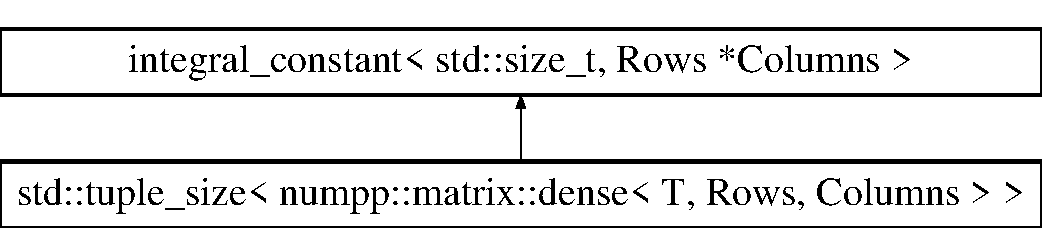
\includegraphics[height=2.000000cm]{classstd_1_1tuple__size_3_01numpp_1_1matrix_1_1dense_3_01T_00_01Rows_00_01Columns_01_4_01_4}
\end{center}
\end{figure}


The documentation for this class was generated from the following file\+:\begin{DoxyCompactItemize}
\item 
structures/matrices/dense/utils.\+hpp\end{DoxyCompactItemize}

\hypertarget{classstd_1_1tuple__size_3_01numpp_1_1vector_3_01T_00_01Size_00_01Tranposition_01_4_01_4}{}\section{std\+:\+:tuple\+\_\+size$<$ numpp\+:\+:vector$<$ T, Size, Tranposition $>$ $>$ Class Template Reference}
\label{classstd_1_1tuple__size_3_01numpp_1_1vector_3_01T_00_01Size_00_01Tranposition_01_4_01_4}\index{std\+::tuple\+\_\+size$<$ numpp\+::vector$<$ T, Size, Tranposition $>$ $>$@{std\+::tuple\+\_\+size$<$ numpp\+::vector$<$ T, Size, Tranposition $>$ $>$}}
Inheritance diagram for std\+:\+:tuple\+\_\+size$<$ numpp\+:\+:vector$<$ T, Size, Tranposition $>$ $>$\+:\begin{figure}[H]
\begin{center}
\leavevmode
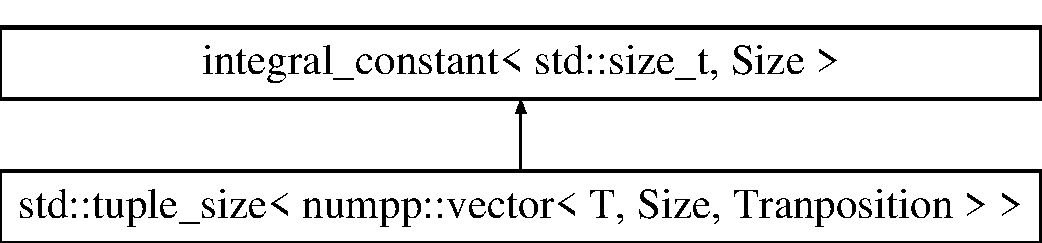
\includegraphics[height=2.000000cm]{classstd_1_1tuple__size_3_01numpp_1_1vector_3_01T_00_01Size_00_01Tranposition_01_4_01_4}
\end{center}
\end{figure}


The documentation for this class was generated from the following file\+:\begin{DoxyCompactItemize}
\item 
structures/vector/utils.\+hpp\end{DoxyCompactItemize}

\hypertarget{classnumpp_1_1differentiation_1_1symbolic_1_1variable}{}\section{numpp\+:\+:differentiation\+:\+:symbolic\+:\+:variable$<$ T, Number $>$ Class Template Reference}
\label{classnumpp_1_1differentiation_1_1symbolic_1_1variable}\index{numpp\+::differentiation\+::symbolic\+::variable$<$ T, Number $>$@{numpp\+::differentiation\+::symbolic\+::variable$<$ T, Number $>$}}


Class representing variable of any type.  




{\ttfamily \#include $<$types.\+hpp$>$}

\subsection*{Public Types}
\begin{DoxyCompactItemize}
\item 
\mbox{\Hypertarget{classnumpp_1_1differentiation_1_1symbolic_1_1variable_a982b8fd32deea706ecd44786a0a4b35a}\label{classnumpp_1_1differentiation_1_1symbolic_1_1variable_a982b8fd32deea706ecd44786a0a4b35a}} 
{\footnotesize template$<$std\+::size\+\_\+t Active$>$ }\\using {\bfseries derivative} = std\+::conditional\+\_\+t$<$ Active==Number, \hyperlink{classnumpp_1_1differentiation_1_1symbolic_1_1constant}{constant}$<$ 1 $>$, \hyperlink{classnumpp_1_1differentiation_1_1symbolic_1_1constant}{constant}$<$ 0 $>$ $>$
\end{DoxyCompactItemize}
\subsection*{Static Public Member Functions}
\begin{DoxyCompactItemize}
\item 
static constexpr auto \hyperlink{classnumpp_1_1differentiation_1_1symbolic_1_1variable_ad73b5d668d3bcf9802a0464ea3389ac6}{calculate} (auto \&\&values)
\begin{DoxyCompactList}\small\item\em Returns value of a certain variable. \end{DoxyCompactList}\end{DoxyCompactItemize}


\subsection{Detailed Description}
\subsubsection*{template$<$typename T, std\+::size\+\_\+t Number$>$\newline
class numpp\+::differentiation\+::symbolic\+::variable$<$ T, Number $>$}

Class representing variable of any type. 


\begin{DoxyTemplParams}{Template Parameters}
{\em T} & type of value in variable (e.\+g. double) \\
\hline
{\em Number} & integer value differentiating variable from every other variable object\\
\hline
\end{DoxyTemplParams}

\begin{DoxyCode}
\textcolor{preprocessor}{#include"numpp/differentiation/symbolic.hpp"}
\end{DoxyCode}
 

\subsection{Member Function Documentation}
\mbox{\Hypertarget{classnumpp_1_1differentiation_1_1symbolic_1_1variable_ad73b5d668d3bcf9802a0464ea3389ac6}\label{classnumpp_1_1differentiation_1_1symbolic_1_1variable_ad73b5d668d3bcf9802a0464ea3389ac6}} 
\index{numpp\+::differentiation\+::symbolic\+::variable@{numpp\+::differentiation\+::symbolic\+::variable}!calculate@{calculate}}
\index{calculate@{calculate}!numpp\+::differentiation\+::symbolic\+::variable@{numpp\+::differentiation\+::symbolic\+::variable}}
\subsubsection{\texorpdfstring{calculate()}{calculate()}}
{\footnotesize\ttfamily template$<$typename T , std\+::size\+\_\+t Number$>$ \\
static constexpr auto \hyperlink{classnumpp_1_1differentiation_1_1symbolic_1_1variable}{numpp\+::differentiation\+::symbolic\+::variable}$<$ T, Number $>$\+::calculate (\begin{DoxyParamCaption}\item[{auto \&\&}]{values }\end{DoxyParamCaption})\hspace{0.3cm}{\ttfamily [inline]}, {\ttfamily [static]}}



Returns value of a certain variable. 

For example\+: 
\begin{DoxyCode}
\textcolor{keyword}{auto} z = \hyperlink{classnumpp_1_1differentiation_1_1symbolic_1_1variable_ad73b5d668d3bcf9802a0464ea3389ac6}{nds::variable<double, 3>::calculate}(\textcolor{keywordtype}{double}[5]\{0,1,2,3,4\});
std::cout << z << std::endl;
\textcolor{comment}{//Will return 2, because it's the 3rd index specified in variable}
\end{DoxyCode}


\begin{DoxyReturn}{Returns}
int 
\end{DoxyReturn}


The documentation for this class was generated from the following file\+:\begin{DoxyCompactItemize}
\item 
differentiation/symbolic/types.\+hpp\end{DoxyCompactItemize}

\hypertarget{classnumpp_1_1vector}{}\section{numpp\+:\+:vector$<$ T, Size, Transposition $>$ Class Template Reference}
\label{classnumpp_1_1vector}\index{numpp\+::vector$<$ T, Size, Transposition $>$@{numpp\+::vector$<$ T, Size, Transposition $>$}}


{\ttfamily \#include $<$structure.\+hpp$>$}

\subsection*{Public Types}
\begin{DoxyCompactItemize}
\item 
\mbox{\Hypertarget{classnumpp_1_1vector_a7b2560fd597d173de79e59646758e494}\label{classnumpp_1_1vector_a7b2560fd597d173de79e59646758e494}} 
using {\bfseries value\+\_\+type} = T
\item 
\mbox{\Hypertarget{classnumpp_1_1vector_aaef4605e241af000e8d48a159972435c}\label{classnumpp_1_1vector_aaef4605e241af000e8d48a159972435c}} 
using {\bfseries size\+\_\+type} = std\+::size\+\_\+t
\item 
\mbox{\Hypertarget{classnumpp_1_1vector_a916b870a14ac1e76e8eab22b5c86d223}\label{classnumpp_1_1vector_a916b870a14ac1e76e8eab22b5c86d223}} 
using {\bfseries difference\+\_\+type} = std\+::ptrdiff\+\_\+t
\item 
\mbox{\Hypertarget{classnumpp_1_1vector_aafa7cc182e3024a9313adc6a04d42302}\label{classnumpp_1_1vector_aafa7cc182e3024a9313adc6a04d42302}} 
using {\bfseries reference} = typename std\+::array$<$ T, Size $>$\+::reference
\item 
\mbox{\Hypertarget{classnumpp_1_1vector_a9c682af3da1dc34cb68c15585b06b19c}\label{classnumpp_1_1vector_a9c682af3da1dc34cb68c15585b06b19c}} 
using {\bfseries const\+\_\+reference} = typename std\+::array$<$ T, Size $>$\+::const\+\_\+reference
\item 
\mbox{\Hypertarget{classnumpp_1_1vector_acf8e239235faf0d77433f8c7133743b8}\label{classnumpp_1_1vector_acf8e239235faf0d77433f8c7133743b8}} 
using {\bfseries pointer} = value\+\_\+type $\ast$
\item 
\mbox{\Hypertarget{classnumpp_1_1vector_af533028c9a99dc86174df15ae28f323a}\label{classnumpp_1_1vector_af533028c9a99dc86174df15ae28f323a}} 
using {\bfseries const\+\_\+pointer} = const value\+\_\+type $\ast$
\item 
\mbox{\Hypertarget{classnumpp_1_1vector_abe494178a87f1be7dfe8078465dc1534}\label{classnumpp_1_1vector_abe494178a87f1be7dfe8078465dc1534}} 
using {\bfseries iterator} = typename std\+::array$<$ T, Size $>$\+::iterator
\item 
\mbox{\Hypertarget{classnumpp_1_1vector_aeb72fcde951bfd845ba24d9f01ec9d14}\label{classnumpp_1_1vector_aeb72fcde951bfd845ba24d9f01ec9d14}} 
using {\bfseries const\+\_\+iterator} = typename std\+::array$<$ T, Size $>$\+::const\+\_\+iterator
\item 
\mbox{\Hypertarget{classnumpp_1_1vector_ab3bb945307c72ee6f5e2b45097a2ed6d}\label{classnumpp_1_1vector_ab3bb945307c72ee6f5e2b45097a2ed6d}} 
using {\bfseries reverse\+\_\+iterator} = typename std\+::array$<$ T, Size $>$\+::reverse\+\_\+iterator
\item 
\mbox{\Hypertarget{classnumpp_1_1vector_a761280bdf7e645f5fe7b7c44cf12fc65}\label{classnumpp_1_1vector_a761280bdf7e645f5fe7b7c44cf12fc65}} 
using {\bfseries const\+\_\+reverse\+\_\+iterator} = typename std\+::array$<$ T, Size $>$\+::const\+\_\+reverse\+\_\+iterator
\end{DoxyCompactItemize}
\subsection*{Public Member Functions}
\begin{DoxyCompactItemize}
\item 
\mbox{\Hypertarget{classnumpp_1_1vector_ad80c07beed6f1f5e24cd5b1b59e71938}\label{classnumpp_1_1vector_ad80c07beed6f1f5e24cd5b1b59e71938}} 
constexpr {\bfseries vector} (const \hyperlink{classnumpp_1_1vector}{vector} \&)=default
\item 
\mbox{\Hypertarget{classnumpp_1_1vector_aaa6ad1b5e7c8f71ff460c296486419a6}\label{classnumpp_1_1vector_aaa6ad1b5e7c8f71ff460c296486419a6}} 
constexpr {\bfseries vector} (\hyperlink{classnumpp_1_1vector}{vector} \&\&)=default
\item 
\mbox{\Hypertarget{classnumpp_1_1vector_a2106f202b6dcf228cbd5c9c5eac519d6}\label{classnumpp_1_1vector_a2106f202b6dcf228cbd5c9c5eac519d6}} 
constexpr \hyperlink{classnumpp_1_1vector}{vector} \& {\bfseries operator=} (const \hyperlink{classnumpp_1_1vector}{vector} \&)=default
\item 
\mbox{\Hypertarget{classnumpp_1_1vector_aea654c76b157b8e826b15ef7da7bccec}\label{classnumpp_1_1vector_aea654c76b157b8e826b15ef7da7bccec}} 
constexpr \hyperlink{classnumpp_1_1vector}{vector} \& {\bfseries operator=} (\hyperlink{classnumpp_1_1vector}{vector} \&\&)=default
\item 
\mbox{\Hypertarget{classnumpp_1_1vector_aa56375d25f669ed670c3d04b844e8424}\label{classnumpp_1_1vector_aa56375d25f669ed670c3d04b844e8424}} 
{\footnotesize template$<$typename... U, typename  = std\+::enable\+\_\+if\+\_\+t$<$						std\+::is\+\_\+same$<$\+T, std\+::common\+\_\+type\+\_\+t$<$\+T, U...$>$$>$\+::value					$>$$>$ }\\constexpr \hyperlink{classnumpp_1_1vector_aa56375d25f669ed670c3d04b844e8424}{vector} (U \&\&... args)
\begin{DoxyCompactList}\small\item\em constructor acting exactly like std\+::initializer\+\_\+list one with type checking \end{DoxyCompactList}\item 
constexpr \hyperlink{classnumpp_1_1vector_ac94f1a73274a498f76425a84cf6e395b}{vector} (const \hyperlink{classnumpp_1_1vector}{vector}$<$ T, Size, !Transposition $>$ \&\hyperlink{classnumpp_1_1vector_a81037f5cce7bd02354efe8b967c191bf}{transposed})
\begin{DoxyCompactList}\small\item\em copy constructor for vector with different transposition \end{DoxyCompactList}\item 
constexpr \hyperlink{classnumpp_1_1vector_aa1ce55da7e9a2ccf1b1624a9f5347d5e}{vector} (\hyperlink{classnumpp_1_1vector}{vector}$<$ T, Size, !Transposition $>$ \&\&\hyperlink{classnumpp_1_1vector_a81037f5cce7bd02354efe8b967c191bf}{transposed})
\begin{DoxyCompactList}\small\item\em move constructor for vector with different transposition \end{DoxyCompactList}\item 
constexpr bool \hyperlink{classnumpp_1_1vector_a81037f5cce7bd02354efe8b967c191bf}{transposed} () const
\item 
\mbox{\Hypertarget{classnumpp_1_1vector_a1e85f0d698ea1fe89382b7f6856e2e9c}\label{classnumpp_1_1vector_a1e85f0d698ea1fe89382b7f6856e2e9c}} 
constexpr std\+::size\+\_\+t {\bfseries size} () const
\item 
\mbox{\Hypertarget{classnumpp_1_1vector_a43212e8baa84331d115e520883329c1e}\label{classnumpp_1_1vector_a43212e8baa84331d115e520883329c1e}} 
constexpr std\+::size\+\_\+t {\bfseries max\+\_\+size} () const
\item 
\mbox{\Hypertarget{classnumpp_1_1vector_a39ba91feb3daa1156002e4e9b58e8ee9}\label{classnumpp_1_1vector_a39ba91feb3daa1156002e4e9b58e8ee9}} 
constexpr bool {\bfseries operator==} (const \hyperlink{classnumpp_1_1vector}{vector} \&x) const
\item 
\mbox{\Hypertarget{classnumpp_1_1vector_a79df8fa5b519885aaae962f2464c0fe6}\label{classnumpp_1_1vector_a79df8fa5b519885aaae962f2464c0fe6}} 
constexpr bool {\bfseries operator!=} (const \hyperlink{classnumpp_1_1vector}{vector} \&x) const
\item 
\mbox{\Hypertarget{classnumpp_1_1vector_ac4a8575eecf2826d5fd3490ca795f007}\label{classnumpp_1_1vector_ac4a8575eecf2826d5fd3490ca795f007}} 
constexpr bool {\bfseries operator==} (const \hyperlink{classnumpp_1_1vector}{vector}$<$ T, Size, !Transposition $>$ \&x) const
\item 
\mbox{\Hypertarget{classnumpp_1_1vector_a87f25e771d021a14b885f8b461f4bbff}\label{classnumpp_1_1vector_a87f25e771d021a14b885f8b461f4bbff}} 
constexpr bool {\bfseries operator!=} (const \hyperlink{classnumpp_1_1vector}{vector}$<$ T, Size, !Transposition $>$ \&x) const
\item 
\mbox{\Hypertarget{classnumpp_1_1vector_a8fe38963af92e47fbc3c60f5206f46a4}\label{classnumpp_1_1vector_a8fe38963af92e47fbc3c60f5206f46a4}} 
constexpr reference {\bfseries operator()} (size\+\_\+type pos)
\item 
\mbox{\Hypertarget{classnumpp_1_1vector_adccd806cababde7552083fd4e6dc1120}\label{classnumpp_1_1vector_adccd806cababde7552083fd4e6dc1120}} 
constexpr const\+\_\+reference {\bfseries operator()} (size\+\_\+type pos) const
\item 
\mbox{\Hypertarget{classnumpp_1_1vector_a4a6a323fba82f8d7e00a97e5c680f3ac}\label{classnumpp_1_1vector_a4a6a323fba82f8d7e00a97e5c680f3ac}} 
constexpr iterator {\bfseries begin} ()
\item 
\mbox{\Hypertarget{classnumpp_1_1vector_abf65526b58940a75270e79e8acb7f9de}\label{classnumpp_1_1vector_abf65526b58940a75270e79e8acb7f9de}} 
constexpr const\+\_\+iterator {\bfseries begin} () const
\item 
\mbox{\Hypertarget{classnumpp_1_1vector_a7a50f2bcccc47bc2cbbc3a14dd4d85cd}\label{classnumpp_1_1vector_a7a50f2bcccc47bc2cbbc3a14dd4d85cd}} 
constexpr const\+\_\+iterator {\bfseries cbegin} () const
\item 
\mbox{\Hypertarget{classnumpp_1_1vector_a554526a327c85c0abc597dff4917b220}\label{classnumpp_1_1vector_a554526a327c85c0abc597dff4917b220}} 
constexpr iterator {\bfseries end} ()
\item 
\mbox{\Hypertarget{classnumpp_1_1vector_a82561fe6ed71bea8de02702a18d3d790}\label{classnumpp_1_1vector_a82561fe6ed71bea8de02702a18d3d790}} 
constexpr const\+\_\+iterator {\bfseries end} () const
\item 
\mbox{\Hypertarget{classnumpp_1_1vector_ac8aecec72fe89e6b818753a2c44ca696}\label{classnumpp_1_1vector_ac8aecec72fe89e6b818753a2c44ca696}} 
constexpr const\+\_\+iterator {\bfseries cend} () const
\item 
\mbox{\Hypertarget{classnumpp_1_1vector_a4f7d7c70486774b877e59c072562a257}\label{classnumpp_1_1vector_a4f7d7c70486774b877e59c072562a257}} 
constexpr reverse\+\_\+iterator {\bfseries rbegin} ()
\item 
\mbox{\Hypertarget{classnumpp_1_1vector_aaf68aef32052dbc490633fc584443e16}\label{classnumpp_1_1vector_aaf68aef32052dbc490633fc584443e16}} 
constexpr const\+\_\+reverse\+\_\+iterator {\bfseries rbegin} () const
\item 
\mbox{\Hypertarget{classnumpp_1_1vector_addd32fda791bcf70bfd1b59669b56858}\label{classnumpp_1_1vector_addd32fda791bcf70bfd1b59669b56858}} 
constexpr const\+\_\+reverse\+\_\+iterator {\bfseries crbegin} () const
\item 
\mbox{\Hypertarget{classnumpp_1_1vector_ad25f7bea977b38be2df1a333063e4dac}\label{classnumpp_1_1vector_ad25f7bea977b38be2df1a333063e4dac}} 
constexpr reverse\+\_\+iterator {\bfseries rend} ()
\item 
\mbox{\Hypertarget{classnumpp_1_1vector_aa077f06cd578ae87860a55b3d1803608}\label{classnumpp_1_1vector_aa077f06cd578ae87860a55b3d1803608}} 
constexpr const\+\_\+reverse\+\_\+iterator {\bfseries rend} () const
\item 
\mbox{\Hypertarget{classnumpp_1_1vector_a953588920df3adbb93c0056f98a6d5cc}\label{classnumpp_1_1vector_a953588920df3adbb93c0056f98a6d5cc}} 
constexpr const\+\_\+reverse\+\_\+iterator {\bfseries crend} () const
\end{DoxyCompactItemize}
\subsection*{Public Attributes}
\begin{DoxyCompactItemize}
\item 
\mbox{\Hypertarget{classnumpp_1_1vector_a470ac88412839d0a338761e13103aa38}\label{classnumpp_1_1vector_a470ac88412839d0a338761e13103aa38}} 
std\+::array$<$ T, Size $>$ {\bfseries vector\+\_\+}
\end{DoxyCompactItemize}


\subsection{Detailed Description}
\subsubsection*{template$<$typename T, std\+::size\+\_\+t Size, bool Transposition = false$>$\newline
class numpp\+::vector$<$ T, Size, Transposition $>$}


\begin{DoxyTemplParams}{Template Parameters}
{\em T} & arithmetic type contained in vector class \\
\hline
{\em Size} & size of the vector \\
\hline
{\em Transposition} & bool indicating whether the vector is transposed\\
\hline
\end{DoxyTemplParams}

\begin{DoxyCode}
\textcolor{preprocessor}{#include"numpp/structures/vector.hpp"}
\end{DoxyCode}
 

\subsection{Constructor \& Destructor Documentation}
\mbox{\Hypertarget{classnumpp_1_1vector_ac94f1a73274a498f76425a84cf6e395b}\label{classnumpp_1_1vector_ac94f1a73274a498f76425a84cf6e395b}} 
\index{numpp\+::vector@{numpp\+::vector}!vector@{vector}}
\index{vector@{vector}!numpp\+::vector@{numpp\+::vector}}
\subsubsection{\texorpdfstring{vector()}{vector()}\hspace{0.1cm}{\footnotesize\ttfamily [1/2]}}
{\footnotesize\ttfamily template$<$typename T, std\+::size\+\_\+t Size, bool Transposition = false$>$ \\
constexpr \hyperlink{classnumpp_1_1vector}{numpp\+::vector}$<$ T, Size, Transposition $>$\+::\hyperlink{classnumpp_1_1vector}{vector} (\begin{DoxyParamCaption}\item[{const \hyperlink{classnumpp_1_1vector}{vector}$<$ T, Size, !Transposition $>$ \&}]{transposed }\end{DoxyParamCaption})\hspace{0.3cm}{\ttfamily [inline]}, {\ttfamily [explicit]}}



copy constructor for vector with different transposition 

Cannot be used in implict casting, you have to cast it explicitly \mbox{\Hypertarget{classnumpp_1_1vector_aa1ce55da7e9a2ccf1b1624a9f5347d5e}\label{classnumpp_1_1vector_aa1ce55da7e9a2ccf1b1624a9f5347d5e}} 
\index{numpp\+::vector@{numpp\+::vector}!vector@{vector}}
\index{vector@{vector}!numpp\+::vector@{numpp\+::vector}}
\subsubsection{\texorpdfstring{vector()}{vector()}\hspace{0.1cm}{\footnotesize\ttfamily [2/2]}}
{\footnotesize\ttfamily template$<$typename T, std\+::size\+\_\+t Size, bool Transposition = false$>$ \\
constexpr \hyperlink{classnumpp_1_1vector}{numpp\+::vector}$<$ T, Size, Transposition $>$\+::\hyperlink{classnumpp_1_1vector}{vector} (\begin{DoxyParamCaption}\item[{\hyperlink{classnumpp_1_1vector}{vector}$<$ T, Size, !Transposition $>$ \&\&}]{transposed }\end{DoxyParamCaption})\hspace{0.3cm}{\ttfamily [inline]}, {\ttfamily [explicit]}}



move constructor for vector with different transposition 

Cannot be used in implict casting, you have to cast it explicitly 

\subsection{Member Function Documentation}
\mbox{\Hypertarget{classnumpp_1_1vector_a81037f5cce7bd02354efe8b967c191bf}\label{classnumpp_1_1vector_a81037f5cce7bd02354efe8b967c191bf}} 
\index{numpp\+::vector@{numpp\+::vector}!transposed@{transposed}}
\index{transposed@{transposed}!numpp\+::vector@{numpp\+::vector}}
\subsubsection{\texorpdfstring{transposed()}{transposed()}}
{\footnotesize\ttfamily template$<$typename T, std\+::size\+\_\+t Size, bool Transposition = false$>$ \\
constexpr bool \hyperlink{classnumpp_1_1vector}{numpp\+::vector}$<$ T, Size, Transposition $>$\+::transposed (\begin{DoxyParamCaption}{ }\end{DoxyParamCaption}) const\hspace{0.3cm}{\ttfamily [inline]}}

returns whether the vector is transposed. \begin{DoxyReturn}{Returns}
true for transposed, false otherwise
\end{DoxyReturn}


The documentation for this class was generated from the following file\+:\begin{DoxyCompactItemize}
\item 
structures/vector/structure.\+hpp\end{DoxyCompactItemize}

%--- End generated contents ---

% Index
\backmatter
\newpage
\phantomsection
\clearemptydoublepage
\addcontentsline{toc}{chapter}{Index}
\printindex

\end{document}
